\documentclass[12pt, letterpaper]{report}

% --- PAQUETES ESENCIALES ---
\usepackage[utf8]{inputenc}
\usepackage[T1]{fontenc}
\usepackage[spanish, es-tabla,es-nodecimaldot]{babel} 

% Soporte para español
\usepackage{geometry}
\usepackage{array}
\usepackage{siunitx}


\newcolumntype{C}[1]{>{\centering\arraybackslash}p{#1}}


\geometry{
    top=3cm,
    bottom=3cm,
    left=2.5cm, % Margen izquierdo un poco más ancho para empastado/anillado
    right=2.5cm
}
\usepackage{graphicx}
\usepackage{amsmath, amssymb} % Herramientas matemáticas y símbolos astronómicos
\usepackage{hyperref}
\usepackage{fancyhdr}
\usepackage[round,authoryear]{natbib} % Estándar para citas en astronomía (ej. Apj, AASTEx)
\usepackage{titlesec}
\usepackage{setspace}
\usepackage{caption}
\captionsetup{font=small}
\usepackage{float}

% Macros de revistas astronómicas para BibTeX (ADS)
\newcommand{\apj}{ApJ}
\newcommand{\apjl}{ApJL}
\newcommand{\apjs}{ApJS}
\newcommand{\aap}{A\&A}
\newcommand{\aapr}{A\&A Rev.}
\newcommand{\aaps}{A\&AS}
\newcommand{\mnras}{MNRAS}
\newcommand{\nat}{Nature}
\newcommand{\araa}{ARA\&A}
\newcommand{\aj}{AJ}
\newcommand{\pasj}{PASJ}
\newcommand{\pasp}{PASP}
\newcommand{\prd}{Phys. Rev. D}
\newcommand{\prl}{Phys. Rev. Lett.}
\newcommand{\icarus}{Icarus}
\newcommand{\planss}{Planet. Space Sci.}

% --- CONFIGURACIÓN DE ESTILO ---

% Configuración de hipervínculos (estilo AASTEx - azul oscuro/cyan)
\hypersetup{
    colorlinks=true,
    linkcolor=blue,
    filecolor=magenta,
    urlcolor=cyan,
    citecolor=blue,
    pdfpagemode=FullScreen,
}

% Diseño de encabezados y pies de página
\pagestyle{fancy}
\fancyhf{}
\fancyhead[R]{\thepage}
\fancyhead[L]{\nouppercase{\leftmark}} % Muestra el nombre del capítulo
\renewcommand{\headrulewidth}{0.4pt}
\renewcommand{\footrulewidth}{0pt}

% Comandos para secciones invisibles (solo aparecen en el índice)
\newcommand{\invisiblesection}[1]{%
  \stepcounter{section}%
  \addcontentsline{toc}{section}{\protect\numberline{\thesection}#1}%
}
\newcommand{\invisiblesubsection}[1]{%
  \stepcounter{subsection}%
  \addcontentsline{toc}{subsection}{\protect\numberline{\thesubsection}#1}%
}
\newcommand{\invisiblesubsubsection}[1]{%
  \stepcounter{subsubsection}%
  \addcontentsline{toc}{subsubsection}{\protect\numberline{\thesubsubsection}#1}%
}

% Formato de los títulos de los capítulos (más limpios y modernos)
\titleformat{\chapter}[display]
  {\normalfont\bfseries\Huge}
  {\chaptertitlename~\thechapter}{20pt}{\Huge}
\titlespacing*{\chapter}{0pt}{-20pt}{40pt}

\begin{document}

% --- PORTADA ---
\begin{titlepage}
\thispagestyle{empty}

%--------------------------------------------------------
% Logo
%--------------------------------------------------------
\begin{flushleft}
    
\includegraphics[width=0.7\textwidth]{figures/logo uc/UC C.GRAY11-03.jpg}
\end{flushleft}

%\vspace{0.2cm}

\begin{center}

{\LARGE\scshape Informe de Práctica\par}

\vspace{0.3cm}

{\Large Licenciatura en Astronomía\par}

\vspace{0.15cm}

{\large Instituto de Astrofísica\par}

\vspace{1.0cm}

\rule{0.80\linewidth}{0.5pt}

\vspace{0.5cm}

{\LARGE\bfseries
Regulación del Flujo de Pebbles por Subestructuras\\[0.15cm]
en Discos Protoplanetarios:\\[0.3cm]
Implicancias para el Crecimiento Planetario\\[0.15cm]
y la Formación de Waterworlds
\par}

\vspace{0.5cm}

\rule{0.80\linewidth}{0.5pt}

\vspace{0.8cm}

{\large\itshape
Un Framework Auto-Consistente de Pebble Accretion\\
Basado en TripodPy
\par}

\vspace{1.8cm}

\begin{minipage}[t]{0.47\textwidth}
\raggedright
\large
\textit{Autor}\\[0.2cm]
\textbf{Maximiliano Felipe\\
Valderrama Vargas}
\end{minipage}
\hfill
\begin{minipage}[t]{0.47\textwidth}
\raggedleft
\large
\textit{Profesor Guía}\\[0.2cm]
\textbf{Prof. Gijs Mulders}
\end{minipage}

\vspace{1.6cm}

{\large Junio de 2026}

\end{center}

\end{titlepage}

% --- PÁGINAS PRELIMINARES ---
\pagenumbering{roman} % Números romanos para el inicio

% Agradecimientos
% =========================================================
% AGRADECIMIENTOS
% =========================================================
\chapter*{Agradecimientos}
\addcontentsline{toc}{chapter}{Agradecimientos}

Quiero expresar mi más sincero agradecimiento a mi profesor guía, el Prof. Gijs Mulders, por su invaluable paciencia, dedicación y constante orientación a lo largo de esta investigación. Su experticia y apoyo fueron fundamentales para la realización de este trabajo.

\vspace{1cm}
A mi familia, por ser mi pilar fundamental y por apoyarme de manera incondicional desde el primer día de esta larga travesía. A mi pareja, Constanza, y a nuestra hija, por iluminar mis días, sacarme tantas risas y darme la energía y perspectiva necesarias para avanzar incluso en las etapas más exigentes de este proceso.

\vspace{1cm}

Finalmente, quisiera expresar mi agradecimiento al clúster Geryon del Centro de Astro-Ingeniería UC, el cual fue una herramienta fundamental para la realización de los cálculos computacionales presentados en este trabajo. Su uso fue posible gracias al apoyo de los proyectos ANID BASAL FB21000, BASAL CATA PFB-06, Anillo ACT-86, FONDEQUIP AIC-57 y QUIMAL 130008, los cuales han contribuido al desarrollo y fortalecimiento de esta infraestructura.


% Índices
\setcounter{tocdepth}{1} % Muestra solo Capítulos (0) y Secciones (1) en el índice
\tableofcontents % Índice general
\newpage


% --- CUERPO DEL INFORME ---
\cleardoublepage
\pagenumbering{arabic} % Cambia a números arábigos
\setstretch{1} % Interlineado de 1.5 para facilitar la lectura al profesor
% =========================================================
% RESUMEN / ABSTRACT
% =========================================================
\chapter*{Resumen}
\addcontentsline{toc}{chapter}{Resumen}
Contexto: La formación de planetas terrestres mediante acreción de pebbles depende críticamente del transporte radial de sólidos en discos protoplanetarios. Sin embargo, la presencia de subestructuras observadas en estos discos puede modificar dicho transporte, alterando tanto el crecimiento planetario como la entrega de agua hacia las regiones internas.

Objetivo: En este trabajo se investiga cómo las trampas de presión y la migración temporal de la línea de nieve regulan el flujo de pebbles y afectan la formación de planetas terrestres y de waterworlds.

Metodología: Para ello se desarrolló un framework auto-consistente basado en TriPoDPy para modelar la evolución de gas y polvo, junto con un módulo de pebble accretion (PA3Py) para calcular el crecimiento de embriones planetarios sobre miles de simulaciones que exploran diferentes configuraciones de turbulencia, subestructuras y propiedades del polvo.

Resultados: Se identificó una \textit{Isla de Crecimiento} en el espacio 
de parámetros ($\alpha \lesssim 10^{-3}$, $M_{\rm gap} \sim 0.1\,M_{\rm Jup}$) 
donde ocurre formación planetaria eficiente. El mecanismo clave es la 
\textit{regulación temporal del flujo de pebbles}: las subestructuras 
controlan no solo cuánto material llega al planeta, sino cuándo lo hace.

Esta modulación temporal genera una correlación entre masa y contenido 
de agua mediante el pebble snow amplificado: liberación tardía de 
reservorios de polvo helado cuando la snowline migra hacia el interior. 
Para muy baja turbulencia ($\alpha = 10^{-4}$), emerge una bifurcación 
poblacional: planetas secos vs ricos en agua, dependiendo de la 
cronología relativa del crecimiento.

Conclusiones: Las subestructuras regulan simultáneamente crecimiento 
y composición planetaria mediante modulación temporal del flujo de 
pebbles. La cronología es tan importante como el inventario de sólidos. 
Estos resultados explican la formación eficiente de planetas terrestres 
ricos en agua en discos estructurados, con predicciones testables 
mediante ALMA.
% =========================================================
% INTRODUCCIÓN
% =========================================================
\chapter{Introducción}
\label{cap:introduccion}

\section{Formación Planetaria y Acreción de Pebbles}

La formación planetaria constituye uno de los problemas fundamentales de la astrofísica moderna. Actualmente se acepta que los planetas se forman en discos protoplanetarios compuestos por gas y polvo que rodean a estrellas jóvenes durante las primeras etapas de su evolución. En estos discos, partículas microscópicas de polvo colisionan y crecen progresivamente hasta formar cuerpos de mayor tamaño, eventualmente dando origen a planetesimales y planetas.

Sin embargo, comprender cómo ocurre este proceso de crecimiento continúa siendo un desafío teórico importante. Los modelos clásicos de acreción enfrentan diversas dificultades, particularmente en las etapas intermedias de crecimiento, donde partículas de tamaño centimétrico a métrico experimentan una rápida deriva radial hacia la estrella central antes de poder formar cuerpos planetarios masivos. Este problema, conocido como la ``drift barrier'', limita significativamente la eficiencia de los modelos tradicionales de formación planetaria \citep{Laibe2012, Blum2018}.

En las últimas décadas, el paradigma de \textit{pebble accretion} ha emergido como una posible solución a estas dificultades. En este escenario, pequeños sólidos aerodinámicamente acoplados al gas ---denominados \textit{pebbles}--- pueden ser acrecidos de manera altamente eficiente por embriones planetarios, acelerando considerablemente el crecimiento de planetas \citep{Lambrechts2014, Bitsch2015, 2019ApJ...883..192A}. Este mecanismo no solo permite explicar escalas temporales compatibles con la vida útil observada de los discos protoplanetarios, sino también reproduce diversas propiedades observadas en sistemas planetarios extrasolares \citep{Johansen2017, Ormel2017, Drazkowska2023, Lyra2023}.


\section{El Problema de los Discos Suaves}

Los modelos modernos de evolución de discos protoplanetarios permiten estudiar cómo evoluciona el flujo de sólidos a lo largo del tiempo y cómo este depende de las propiedades físicas del disco. Frameworks como \textit{Pebble Predictor} \citep{Drazkowska2021} modelan la evolución del gas y del polvo, permitiendo calcular el flujo radial de pebbles hacia distintas regiones del disco protoplanetario. Asimismo, herramientas más recientes como \textit{TripodPy} \citep{Pfeil2024_teoria, Pfeil2025_codigo} permiten incorporar modelos avanzados de evolución de polvo y distribuciones de tamaño multipoblacionales.

Estos resultados pueden posteriormente utilizarse como input para modelos de \textit{pebble accretion} o esquemas de postprocesado orientados a estudiar el crecimiento de embriones planetarios y la evolución composicional de sistemas planetarios.

Sin embargo, muchos de estos modelos asumen discos protoplanetarios suaves (\textit{smooth disks}), es decir, discos con perfiles radiales continuos y sin subestructuras locales. Esta aproximación presenta limitaciones importantes desde el punto de vista físico.

En discos suaves, los pebbles experimentan una rápida deriva radial producto del acoplamiento aerodinámico con el gas. Debido a que el gas orbita a velocidades ligeramente sub-Keplerianas, las partículas sólidas sienten un \textit{headwind} que les hace perder momento angular y migrar hacia la estrella central. En ausencia de trampas de presión o estructuras capaces de modificar localmente el gradiente de presión, este proceso produce un transporte eficiente y continuo de sólidos hacia las regiones internas del disco.

Como consecuencia, los modelos \textit{smooth} pueden sobreestimar el flujo de pebbles disponible para acreción planetaria en el disco interno, afectando significativamente las predicciones sobre crecimiento planetario y eficiencia de acreción \citep{Lau2024, Appelgren2020, Appelgren2025}.

En este contexto, incorporar subestructuras en modelos de evolución de discos resulta fundamental para construir escenarios más realistas de formación planetaria. Las perturbaciones locales del perfil de presión pueden modificar significativamente el transporte de sólidos y regular el flujo de pebbles a través del disco.


\section{Subestructuras en Discos Protoplanetarios}

Observaciones de alta resolución realizadas durante la última década han revolucionado nuestra comprensión de los discos protoplanetarios. En particular, el observatorio ALMA (\textit{Atacama Large Millimeter/submillimeter Array}) ha revelado que numerosos discos presentan complejas subestructuras radiales, incluyendo anillos, gaps, cavidades y regiones localizadas de acumulación de polvo \citep{ALMAPartnership2015, Andrews2018}.

Uno de los ejemplos más emblemáticos corresponde al disco protoplanetario de HL Tauri, cuyas observaciones mostraron por primera vez una serie de anillos y gaps bien definidos incluso en etapas tempranas de evolución del disco \citep{ALMAPartnership2015}. Posteriormente, múltiples estudios confirmaron que este tipo de estructuras son comunes en discos protoplanetarios observados a longitudes de onda milimétricas \citep{Andrews2018}.


\begin{figure}[ht]
    \centering
    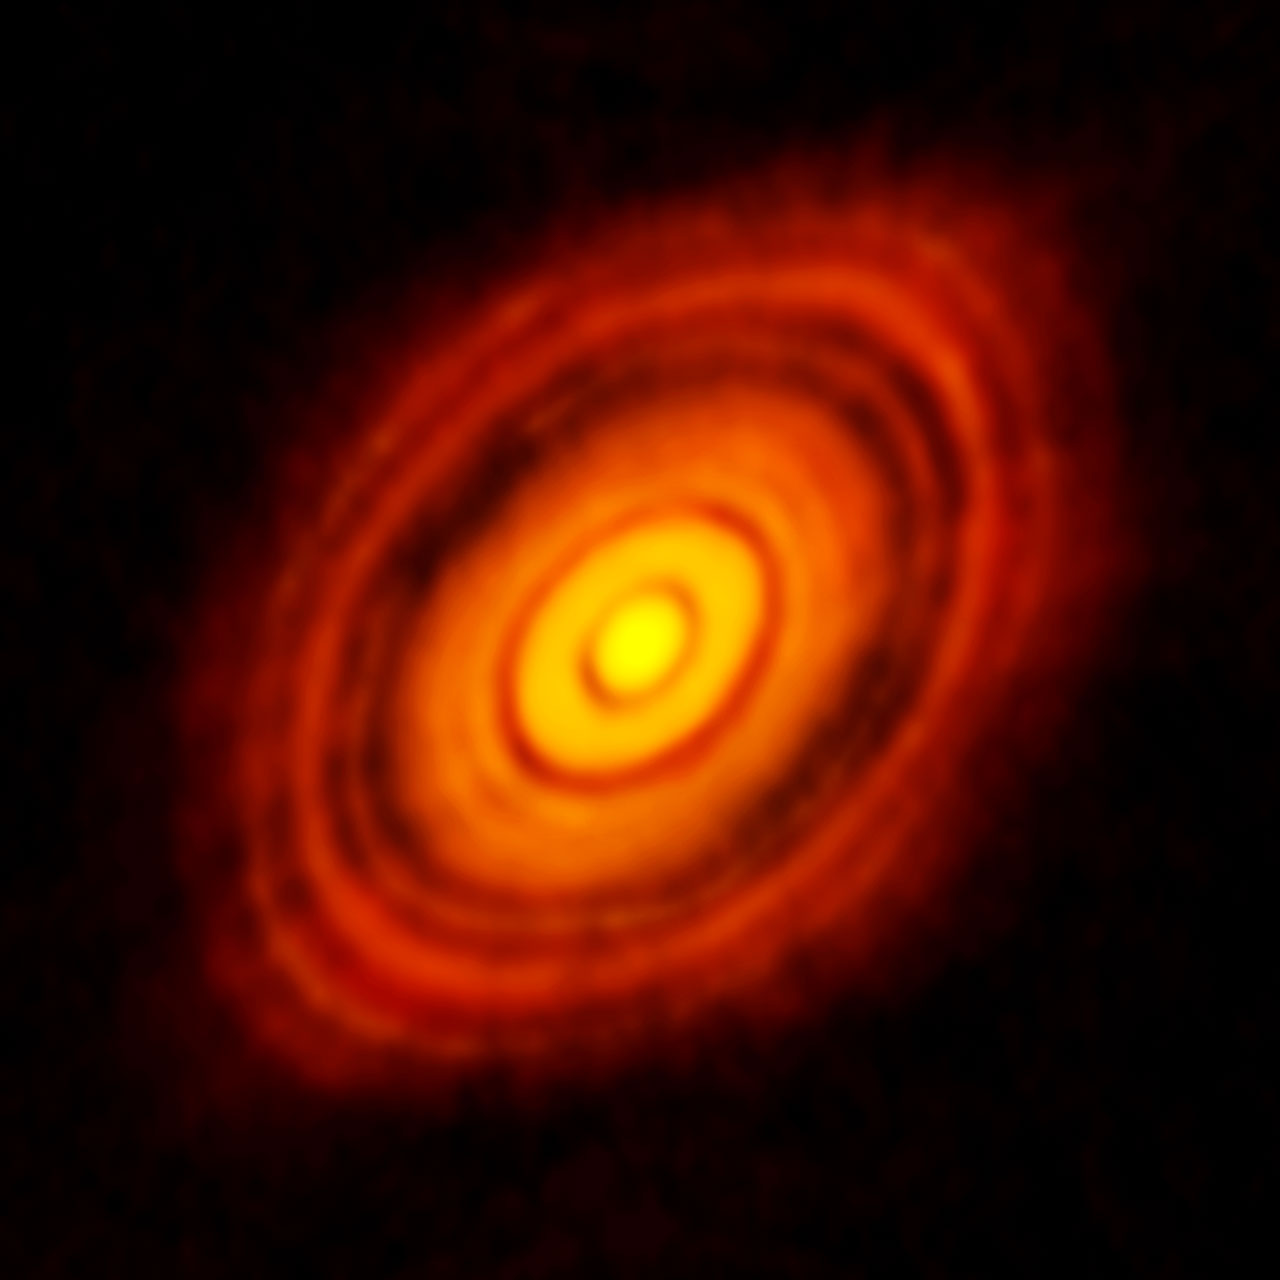
\includegraphics[width=0.8\textwidth]{figures/HL tauri.jpg}
    \caption{Disco protoplanetario alrededor de HL Tauri observado con ALMA. La imagen revela estructuras anulares y regiones oscuras asociadas con posibles procesos de formación planetaria. Creditos: ALMA (ESO/NAOJ/NRAO).}
    \label{fig:HLTau}
\end{figure}


Diversos mecanismos físicos han sido propuestos para explicar el origen de estas subestructuras. Entre ellos se incluyen la interacción disco-planeta, inestabilidades magnetohidrodinámicas, variaciones locales de viscosidad asociadas a \textit{dead zones}, transiciones químicas cercanas a \textit{snowlines} y procesos hidrodinámicos capaces de modificar localmente el perfil de presión del gas \citep{Akiyama2016, Andrews2018, Kanagawa2016}.

Desde el punto de vista dinámico, estas estructuras pueden actuar como trampas de presión (\textit{pressure bumps}) capaces de alterar significativamente el transporte radial de sólidos. En regiones donde el gradiente de presión cambia de signo o disminuye localmente, la deriva radial de pebbles puede ralentizarse o incluso detenerse temporalmente, favoreciendo la acumulación de polvo y reduciendo el flujo de material sólido hacia el interior del disco \citep{Pinilla2012, Pierens2024, Baruteau2019}.

Como consecuencia, las subestructuras no solo modifican la distribución espacial de sólidos, sino también las condiciones bajo las cuales ocurre \textit{pebble accretion} \citep{Andama2022, Ataiee2018}. Esto puede impactar directamente las escalas temporales de crecimiento planetario, la eficiencia de acreción y la composición final de los planetas formados.


\section{Pebble Flux y Composición Planetaria}

El flujo radial de pebbles constituye uno de los parámetros más importantes en modelos modernos de formación planetaria. La cantidad de material sólido transportado a través del disco determina directamente la masa disponible para acreción planetaria y, por lo tanto, controla las escalas temporales y la eficiencia del crecimiento de embriones planetarios.

Además de regular el crecimiento, el \textit{pebble flux} también juega un rol fundamental en la composición final de los planetas. A medida que los pebbles migran radialmente a través del disco, atraviesan distintas regiones térmicas donde materiales volátiles pueden condensarse o sublimarse. En particular, la \textit{snowline} del agua representa una transición crítica para la distribución composicional de sólidos en discos protoplanetarios.

La evolución temporal de estas regiones puede modificar significativamente la composición de los pebbles disponibles para acreción \citep{Booth2017, Booth2019}. Como consecuencia, cambios en el transporte radial de sólidos pueden producir variaciones importantes en el contenido de agua y volátiles de los planetas formados \citep{Banzatti2023}.

En este contexto, diversos trabajos han propuesto que mecanismos capaces de regular el flujo de pebbles podrían favorecer la formación de planetas ricos en agua, comúnmente denominados \textit{waterworlds} \citep{McCloat2025, Krijt2025, Bitsch2021, Astrakhantsev2026}. Comprender cómo las subestructuras afectan el transporte de sólidos resulta, por tanto, fundamental para estudiar la conexión entre dinámica de discos protoplanetarios y composición planetaria.


\section{Transporte Tardío de Agua y Rol de las Subestructuras}

Aunque diversos estudios han mostrado que el transporte radial de pebbles puede desempeñar un papel importante en la composición de los planetas formados, la mayoría de estos escenarios asumen un suministro relativamente continuo de material sólido hacia las regiones internas del disco \citep{Appelgren2020, Lau2024}.

Sin embargo, la presencia de subestructuras observadas en discos protoplanetarios introduce la posibilidad de que el flujo de pebbles sea modulado temporalmente \citep{Pinilla2012, Stammler2022}. En particular, la retención de polvo en reservorios asociados a gaps podría retrasar la llegada de material rico en volátiles hasta etapas más avanzadas de evolución del disco, cuando la \textit{snowline} del agua se encuentra más cerca de la región terrestre \citep{Oka2011, Bitsch2015}.

Esto plantea la posibilidad de que la interacción entre la evolución de la \textit{snowline} y la liberación de estos reservorios tenga consecuencias importantes sobre la entrega tardía de agua y la composición final de los planetas \citep{Banzatti2023, McCloat2025}.


\subsection{Hipótesis de Trabajo}

En este trabajo se propone que la retención temporal de pebbles producida por subestructuras de origen planetario puede retrasar la llegada de material rico en volátiles hacia las regiones internas del disco. Si la \textit{snowline} atraviesa estos reservorios antes de que sean completamente liberados, el cambio en las propiedades de fragmentación del polvo puede desencadenar una liberación tardía de pebbles, fenómeno conocido como \textit{pebble snow} \citep{Drazkowska2021, McCloat2025}.

Se plantea que este mecanismo puede modificar significativamente el flujo de sólidos disponible para acreción planetaria y favorecer el transporte tardío de agua hacia regiones cercanas a la zona habitable, afectando tanto el crecimiento como la composición final de los planetas formados \citep{Bitsch2021, Krijt2025, Astrakhantsev2026}.

\section{Objetivos del Trabajo}

Con el objetivo de evaluar esta hipótesis, se desarrolló un framework computacional basado en TripodPy capaz de modelar discos protoplanetarios estructurados mediante perturbaciones locales del perfil de presión del gas.

A partir de estas simulaciones, se analizó cómo distintas configuraciones de gaps y \textit{pressure bumps} afectan el transporte radial de sólidos y la evolución temporal del \textit{pebble flux}.

Adicionalmente, se desarrolló un esquema de postprocesado orientado a estudiar acreción de pebbles y evolución composicional, incorporando efectos asociados a la migración de la \textit{snowline} y al transporte diferencial de materiales volátiles.

Finalmente, este trabajo busca explorar si la regulación del flujo de pebbles producida por subestructuras puede favorecer escenarios de formación de planetas ricos en agua y modificar las predicciones tradicionales de modelos basados en discos suaves.

% =========================================================
% MARCO TEÓRICO
% =========================================================

\chapter{Marco Teórico}
\label{cap:marco_teorico}

% ---------------------------------------------------------
% Evolución del polvo
% ---------------------------------------------------------
% ---------------------------------------------------------
% Evolución de Polvo en Discos Protoplanetarios
% ---------------------------------------------------------
\section{Evolución de Polvo en Discos Protoplanetarios}

\invisiblesubsection{Crecimiento y Fragmentación}

En el paradigma estándar de formación planetaria, los granos submicrométricos heredados del medio interestelar constituyen la materia prima a partir de la cual se forman los planetas. Durante las primeras etapas de evolución del disco protoplanetario, estas partículas crecen mediante colisiones a bajas velocidades relativas, dominadas por fuerzas de Van der Waals \citep{Dominik1997,Blum2018}. A medida que los agregados aumentan de tamaño, la turbulencia y las velocidades diferenciales incrementan la energía de las colisiones. Cuando esta supera la energía de cohesión del material, las colisiones dejan de producir crecimiento y pasan a estar dominadas por fragmentación. Este proceso establece un tamaño máximo para las partículas sólidas, conocido como \textit{fragmentation barrier} \citep{Birnstiel2012, Blum2018, Drazkowska2023}, que puede aproximarse mediante

\begin{equation}
a_{\rm frag} \propto
\frac{\Sigma_g}{\rho_s,\alpha}
\frac{v_{\rm frag}^2}{c_s^2},
\end{equation}

donde $\Sigma_g$ es la densidad superficial del gas, $\rho_s$ la densidad interna de los sólidos, $\alpha$ el parámetro turbulento de \citet{Shakura_sunyaev_1973}, $c_s$ la velocidad local del sonido y $v_{\rm frag}$ la velocidad crítica de fragmentación. Esta última depende fuertemente de la composición del material, alcanzando valores del orden de $\sim10{\rm ms^{-1}}$ para partículas recubiertas por hielo \citep{Gundlach_2014} y de $\sim1{\rm ms^{-1}}$ para silicatos secos \citep{Blum2018, Musiolik_Grzegorz_Gerhard2019}. En consecuencia, materiales más resistentes y discos menos turbulentos favorecen la formación de pebbles de mayor tamaño.

Además de estar limitados por fragmentación, los pebbles milimétricos y centimétricos experimentan una rápida deriva radial debido a su interacción aerodinámica con el gas. Este proceso da origen a la denominada \textit{drift barrier}, una de las principales dificultades que enfrentan los modelos clásicos de formación planetaria, ya que las partículas pueden migrar hacia la estrella central antes de incorporarse a cuerpos de mayor tamaño \citep{Laibe2012, Blum2018}.


\invisiblesubsection{Número de Stokes y Acoplamiento Aerodinámico}

 El grado de acoplamiento de una partícula con el flujo de gas se cuantifica a través del número de Stokes ($St$), definido como:
\begin{equation}
St = t_{\rm stop} \Omega_{\rm K}
\end{equation}
donde $t_{\rm stop}$ representa el tiempo de frenado aerodinámico y $\Omega_{\rm K}$ la frecuencia orbital Kepleriana local \citep{Weidenschilling1977, Birnstiel2012}.

El régimen de Epstein aplica cuando el tamaño de la partícula satisface:
\begin{equation}
a \lesssim \frac{9}{4}\lambda_{\rm mfp}
\end{equation}
donde $\lambda_{\rm mfp}$ corresponde al camino libre medio de las moléculas del gas. Este régimen domina en gran parte de los discos protoplanetarios.

Partículas muy pequeñas ($St \ll 1$) se encuentran fuertemente acopladas al gas, mientras que cuerpos masivos ($St \gg 1$) evolucionan de manera prácticamente Kepleriana. Los \textit{pebbles} ($St \sim 0.01 - 1$) se ubican en un régimen intermedio donde la interacción aerodinámica alcanza su máxima eficiencia.

\invisiblesubsection{Altura de Escala del Polvo}

La sedimentación de los sólidos hacia el plano medio del disco está determinada por el equilibrio entre la gravedad vertical del campo estelar y la difusión turbulenta. La altura de escala del gas viene dada por

\begin{equation}
H_g=\frac{c_s}{\Omega_{\rm K}},
\end{equation}

donde $c_s$ corresponde a la velocidad local del sonido y $\Omega_{\rm K}$ a la frecuencia angular Kepleriana \citep{Birnstiel2012, Ormel2017}. Esta cantidad caracteriza el espesor vertical del disco y determina la distribución de los sólidos alrededor del plano medio.

Como resultado de la sedimentación, la altura de escala de la capa de pebbles es significativamente menor que la del gas \citep{Birnstiel2012, Ormel2017}:

\begin{equation}
H_{\rm peb} = H_g \sqrt{\frac{\alpha}{\alpha + St}}
\end{equation}

donde $\alpha$ es el parámetro de turbulencia y $St$ el número de Stokes de las partículas. Esta expresión muestra que partículas con valores elevados de $St$ sedimentan más eficientemente, formando una capa delgada y densa.

La altura de escala de los pebbles determina además el régimen de acreción. Cuando el radio efectivo de captura del embrión satisface $b_{\rm col}\lesssim H_{\rm peb}$, el sistema opera en el régimen tridimensional (3D), mientras que para $b_{\rm col}\gtrsim H_{\rm peb}$ la acreción transita al régimen bidimensional (2D).


\invisiblesubsection{Deriva Radial de Pebbles}

El disco de gas posee soporte térmico generado por su gradiente de presión radial negativo. Como consecuencia, el gas orbita a velocidades ligeramente sub-Keplerianas:
\begin{equation}
v_{\rm gas} = v_{\rm K}(1-\eta)
\end{equation}
donde $\eta$ cuantifica la desviación respecto a la velocidad Kepleriana y puede expresarse como:
\begin{equation}
\eta = -\frac{1}{2}\left(\frac{c_s}{v_{\rm K}}\right)^2 \frac{\partial \ln P}{\partial \ln r}
\end{equation}

Dado que las partículas sólidas no sienten directamente el soporte de presión, tienden a moverse a velocidades Keplerianas y experimentan un \textit{headwind} continuo. Esta interacción extrae momento angular de los sólidos y produce migración radial hacia la estrella \citep{Birnstiel2012, Laibe2012}. La velocidad radial de deriva se aproxima mediante:
\begin{equation}
v_r = -\frac{2\eta v_{\rm K} St}{1+St^2}
\end{equation}

La deriva alcanza su máxima eficiencia para partículas marginalmente acopladas ($St \approx 1$). En muchos casos, esta migración radial limita el crecimiento antes de alcanzar el régimen de fragmentación. Bajo esta condición, el tamaño máximo impuesto por deriva radial se aproxima como:
\begin{equation}
a_{\rm drift} \propto \frac{\Sigma_d}{\rho_s}
\left(\frac{v_{\rm K}}{c_s}\right)^2
\left|\frac{\partial \ln P}{\partial \ln r}\right|^{-1}
\end{equation}
donde $\Sigma_d$ es la densidad superficial de polvo.

Las escalas temporales de deriva radial son considerablemente menores que las escalas de coagulación, lo que conduciría a una rápida acreción estelar del material sólido si no existiesen mecanismos capaces de detener este transporte radial.


% ---------------------------------------------------------

\section{Subestructuras y Trampas de Presión}
\label{sec:subestructuras}

\invisiblesubsection{Origen de Pressure Bumps}

En contraste con la visión clásica de discos suaves, las observaciones modernas muestran que los discos protoplanetarios presentan anillos, gaps y múltiples subestructuras radiales \citep{ALMAPartnership2015, Andrews2018}. Estas perturbaciones locales del perfil de presión, conocidas como \textit{pressure bumps}, pueden originarse mediante diversos mecanismos físicos.

Entre los mecanismos más importantes se encuentra la interacción gravitacional entre el disco y planetas masivos embebidos, capaces de abrir gaps y generar máximos locales de presión en los bordes externos de sus órbitas \citep{Kanagawa2016}. Asimismo, procesos hidrodinámicos e inestabilidades magnetohidrodinámicas también pueden producir estructuras similares. En particular, las variaciones abruptas de viscosidad en regiones de baja ionización (\textit{dead zones}) favorecen acumulaciones locales de gas que alteran significativamente el perfil de presión del disco.

Desde el punto de vista morfológico, el perfil de un gap inducido por un planeta masivo puede modelarse analíticamente. El modelo de \citet{Kanagawa2016} relaciona el ancho y la profundidad del gap con la masa del planeta y los parámetros viscosos del disco. El perfil de \citet{Duffell2020} complementa esta descripción, proporcionando una función suave que reproduce fielmente los resultados de simulaciones hidrodinámicas de alta resolución. En ambos casos, el borde externo del gap actúa como una trampa de presión natural capaz de retener sólidos e interrumpir el flujo de pebbles hacia la estrella \citep{Pinilla2012, Baruteau2019}.

\invisiblesubsection{Filtrado de Pebbles}

En un disco suave, el gradiente de presión negativo induce una rápida deriva radial de pebbles hacia la estrella. Sin embargo, en presencia de un \textit{pressure bump}, el gradiente de presión puede invertirse localmente.

En estas regiones, el gas alcanza velocidades cercanas o incluso superiores a la velocidad Kepleriana, empujando aerodinámicamente a las partículas hacia el máximo de presión. Como consecuencia, los pebbles quedan atrapados y su transporte radial se modifica sustancialmente \citep{Pinilla2012, Ataiee2018}.

\invisiblesubsection{Impacto sobre el Flujo Sólido}

La acumulación de sólidos en trampas de presión incrementa localmente la razón polvo-gas y favorece la formación de planetesimales \citep{Carrera2021} por mecanismos de colapso gravitacional colectivo.

Esta retención implica una reducción significativa del flujo radial de pebbles disponible para el disco interno, la cual modifica directamente las condiciones de crecimiento de planetesimales interiores, afectando tanto las tasas de acreción como la composición final de los planetas formados.

Este mecanismo constituye la motivación central del presente trabajo, el cual explora cómo distintas configuraciones de subestructuras y parámetros turbulentos alteran el transporte de sólidos en discos protoplanetarios.

% ---------------------------------------------------------

\section{Pebble Accretion}
\label{sec:pebble_accretion}

\invisiblesubsection{Masa de Inicio}

Para que un embrión planetario (planetesimal) entre al régimen de \textit{pebble accretion}, debe superar una masa crítica conocida como masa de inicio (\textit{onset mass}). Por debajo de este umbral, las interacciones entre pebbles y el cuerpo planetario son predominantemente balísticas y poco eficientes.

Una vez alcanzada esta masa, la gravedad del embrión y el arrastre aerodinámico permiten disipar energía cinética de los pebbles, aumentando drásticamente la sección eficaz de acreción e iniciando una fase de crecimiento altamente eficiente \citep{Lambrechts2014, Ormel2017}.

\invisiblesubsection{Regímenes de Acreción}

A medida que el planeta crece, la acreción transita entre distintos regímenes geométricos y dinámicos \citep{Ormel2017}.

Geométricamente, la acreción evoluciona desde un régimen tridimensional (3D), donde el radio efectivo de acreción es menor que la altura de escala del polvo ($H_{\rm peb}$), hacia un régimen bidimensional (2D), donde el planeta interactúa con prácticamente toda la capa de pebbles.

Cinemáticamente, el sistema transita desde el régimen de \textit{headwind}, dominado por deriva aerodinámica, hacia el régimen de \textit{shear}, donde domina la cizalla Kepleriana local.

En el régimen bidimensional, la tasa de acreción puede aproximarse como:
\begin{equation}
\dot{M}_{\rm PA} \sim 2 R_{\rm acc} v_{\rm rel} \Sigma_{\rm peb}
\end{equation}
donde $R_{\rm acc}$ es el radio efectivo de acreción, $v_{\rm rel}$ la velocidad relativa entre pebbles y planeta, y $\Sigma_{\rm peb}$ la densidad superficial de sólidos \citep{Lambrechts2014}.

\invisiblesubsection{Flujo Radial de Pebbles}

El flujo de masa sólida transportado radialmente hacia la estrella se define como:
\begin{equation}
\dot{M}_{\rm peb} = 2\pi r \Sigma_{\rm peb} v_r
\end{equation}
donde $\Sigma_{\rm peb}$ corresponde a la densidad superficial de pebbles y $v_r$ a su velocidad radial. La disponibilidad de este flujo es el factor limitante del crecimiento por pebble accretion: una reducción de $\dot{M}_{\rm peb}$ ---por ejemplo, causada por una trampa de presión exterior--- puede frenar o detener el crecimiento del embrión antes de alcanzar la masa de aislamiento \citep{Lambrechts2014}.

\invisiblesubsection{Masa de Aislamiento}

A medida que el planeta incrementa su masa, su perturbación gravitacional sobre el disco modifica localmente el perfil de presión del gas, formando un \textit{pressure bump} exterior que bloquea el flujo entrante de pebbles.

La masa planetaria a la cual ocurre este fenómeno se conoce como masa de aislamiento:
\begin{equation}
    M_{\rm iso} \propto \left(\frac{H}{r}\right)^3 M_*
\end{equation}
donde $H/r$ es la razón de aspecto del disco y $M_*$ la masa estelar \citep{Lambrechts2014, Ormel2017, Ataiee2018, Bitsch2015}.

La masa de aislamiento marca el fin del crecimiento eficiente mediante pebble accretion y puede representar el inicio de la acreción significativa de envoltura gaseosa.

% ---------------------------------------------------------

\section{Snowline y Evolución Composicional}

\invisiblesubsection{Migración de la Línea de Nieve}

Las propiedades térmicas del disco generan regiones de condensación para distintos compuestos volátiles. La más importante corresponde a la snowline del agua, localizada aproximadamente donde:
\begin{equation}
T_{\rm snow} \sim 170 \ {\rm K}
\end{equation}

Durante etapas tempranas del disco, el calentamiento viscoso desplaza esta línea hacia regiones externas. Conforme el disco evoluciona y se enfría —a medida que la tasa de acreción estelar $\dot{M}_\star$ disminuye progresivamente— la snowline migra hacia radios menores \citep{Hartmann1998, Oka2011}.

Esta evolución temporal modifica continuamente las regiones del disco capaces de aportar material rocoso o material rico en hielos durante el crecimiento planetario.

\invisiblesubsection{Fragmentación Dependiente de Composición}

La velocidad crítica de fragmentación depende fuertemente de la composición físico-química de las partículas \citep{Gundlach_2014, Blum2018, Musiolik_Grzegorz_Gerhard2019, Drazkowska2023}.

Fuera de la snowline, los mantos de hielo aumentan significativamente la adhesividad del material \citep{Gundlach_2014}, permitiendo velocidades críticas del orden de:
\begin{equation}
v_{\rm frag} \sim 10 \ {\rm m/s}
\end{equation}

En el interior de la snowline, la sublimación del hielo deja partículas secas dominadas por silicatos, mucho más frágiles \citep{Blum2018, Musiolik_Grzegorz_Gerhard2019}:
\begin{equation}
v_{\rm frag} \sim 1 \ {\rm m/s}
\end{equation}

Como consecuencia, el tamaño máximo y el número de Stokes de los sólidos decrecen significativamente en las regiones internas del disco.

\invisiblesubsection{Pebble Snow y Waterworlds}

La deriva radial de pebbles transporta continuamente material rico en volátiles desde el disco externo hacia regiones internas, enriqueciendo químicamente tanto el gas como los sólidos interiores \citep{Booth2017, Booth2019}. Este proceso, conocido como \textit{pebble snow}, ha sido detectado observacionalmente a través de exceso de vapor de agua frío cerca de la snowline en discos compactos \citep{Banzatti2023}.

Cuando partículas heladas cruzan la snowline, el hielo sublima e inyecta vapor de agua al gas del disco. Sin embargo, embriones localizados justo fuera de esta frontera pueden interceptar eficientemente pebbles ricos en hielo antes de su sublimación.

La acreción sostenida de este material permite incorporar enormes cantidades de agua a los núcleos planetarios, favoreciendo la formación de planetas con fracciones de agua significativamente superiores a las del Sistema Solar, conocidos como \textit{waterworlds} \citep{Bitsch2021, McCloat2025, Drazkowska2023}.

% ---------------------------------------------------------

\section{Impacto de las Subestructuras sobre el Flujo de Pebble}

Dado que las subestructuras modifican el transporte radial de sólidos, comprender cómo distintas configuraciones de \textit{pressure bumps} alteran el \textit{pebble flux} resulta fundamental para construir modelos más realistas de formación planetaria.

En este trabajo se estudia el impacto de distintas configuraciones de subestructuras y parámetros turbulentos sobre la evolución del flujo de pebbles utilizando simulaciones numéricas de evolución de polvo y gas en discos protoplanetarios.

% =========================================================
% METODOLOGÍA
% =========================================================

\chapter{Metodología Computacional}
\label{cap:metodologia}


% ---------------------------------------------------------
% Framework base
% ---------------------------------------------------------

\section{Framework Base: Modelado de Discos 1D}
\label{sec: tripodpy}
La evolución del disco protoplanetario se modeló utilizando \texttt{TriPoDPy} \citep{Pfeil2024_teoria, Kaufmann2025}, un framework desarrollado en Python que resuelve de manera acoplada la evolución viscosa del gas, el transporte radial del polvo y los procesos de coagulación y fragmentación en una dimensión radial. 

\invisiblesubsection{TriPoDPy y las Poblaciones de Polvo}

La resolución completa de la ecuación de coagulación de Smoluchowski \citep{Smoluchowski1916} resulta computacionalmente costosa. Para reducir este costo, \texttt{TriPoDPy} \citep{Pfeil2024_teoria, Kaufmann2025} aproxima la distribución local de tamaños mediante tres poblaciones características: granos pequeños ($a_0$), partículas intermedias ($a_1$) y pebbles correspondientes al tamaño máximo local ($a_{\rm max}$). Esta representación paramétrica permite describir la evolución del polvo con un costo computacional considerablemente menor.

\invisiblesubsection{Configuración Numérica y Condiciones Iniciales}

Las simulaciones se realizaron sobre una grilla radial logarítmica. Los parámetros globales y las configuraciones exploradas se resumen en la Tabla~\ref{tab:parametros_globales}.

\begin{table*}[t]
\centering
\caption{Parámetros globales del modelo. Los valores entre corchetes indican los rangos explorados en los barridos poblacionales.}
\small

\begin{tabular}{C{2.5cm}C{3.8cm}p{8.8cm}}
\hline\hline
Símbolo & Valor [Rango] & Descripción \\
\hline

\multicolumn{3}{c}{\textit{Estrella y disco}}\\
\hline

$M_*$ &
$1.0\,M_\odot$ &
Masa de la estrella central. \\

$R_*$ &
$2.1\,R_\odot$ &
Radio estelar inflado correspondiente a la fase de pre-secuencia principal. \\

$T_{\rm eff}$ &
$4000\,\mathrm{K}$ &
Temperatura efectiva que determina la estructura térmica del disco. \\

$M_{\rm disk}/M_*$ &
0.05 &
Fracción de masa inicial del disco. \\

$R_c$ &
$30.0\,\mathrm{AU}$ &
Radio característico asociado al decaimiento exponencial de la densidad superficial del gas. \\

$\alpha$ &
$10^{-3}\,[10^{-4}-10^{-2}]$ &
Parámetro de viscosidad turbulenta de Shakura--Sunyaev. \\

$R_{\rm in}-R_{\rm out}$ &
$0.5-100\,\mathrm{AU}$ &
Límites interno y externo del dominio radial. \\

$N_r$ &
300 &
Número de celdas de la grilla radial logarítmica. \\

\hline
\multicolumn{3}{c}{\textit{Embriones planetarios}}\\
\hline

$n_{\rm emb}$ &
1 &
Número de embriones por simulación. \\

$M_{\rm emb, 0}$ &
$10^{-4}\,M_\oplus\,[10^{-5}-10^{-2}]$ &
Masa inicial del embrión planetario. \\

$r_{\rm seed}$ &
$1.0\,\mathrm{AU}$ &
Ubicación radial del embrión. \\

\hline
\multicolumn{3}{c}{\textit{Gaps y subestructuras}}\\
\hline

$M_{\rm gap}$ &
$0.1\,M_{\rm Jup}\,[0.01-5.0]$ &
Masa del planeta gigante responsable de abrir el gap. \\

$r_{\rm gap}$ &
$10.0\,\mathrm{AU}\,[5.0-30.0]$ &
Ubicación radial del gap. \\

$A_{\rm sin}$ &
$[0.5-5.0]$ &
Amplitud de las perturbaciones sinusoidales. \\

\hline
\multicolumn{3}{c}{\textit{Línea de nieve y polvo}}\\
\hline

$v_{\rm frag}$ &
$1.0 \rightarrow 1.0-3.0-10.0\,\mathrm{m\,s^{-1}}$&
Velocidad umbral de fragmentación para silicatos en la región interior y hielos en la región exterior. \\

$r_{\rm SL}$ &
$\sim 2.7 \rightarrow 0.5\,\mathrm{AU}$ &
Evolución temporal de la posición de la línea de nieve. \\

\hline
\end{tabular}
\label{tab:parametros_globales}
\end{table*}


Finalmente, no se incorporó un modelo auto-consistente de evolución de la luminosidad estelar acoplado a la hidrodinámica del disco. La inclusión de un tratamiento termodinámico iterativo incrementaría significativamente el costo computacional de las simulaciones. Por esta razón, la evolución temporal de la \textit{snowline} se parametrizó de forma independiente, como se describe en la Sección~\ref{sec:snowline}. Esta aproximación permite reproducir de manera razonable la migración de la línea de nieve sin modificar la estructura hidrodinámica calculada por \texttt{TriPoDPy}.


% ---------------------------------------------------------
% Subestructuras
% ---------------------------------------------------------
\section{Implementación de Discos Estructurados}

Con el objetivo de modelar subestructuras asociadas a \textit{gaps} abiertos por planetas gigantes, se introdujeron perturbaciones locales en el parámetro de viscosidad turbulenta $\alpha$ de Shakura--Sunyaev \citep{Shakura_sunyaev_1973}. Los perfiles de gap se calcularon utilizando las parametrizaciones propuestas por \citet{Kanagawa2016} y \citet{Duffell2020}. En este trabajo se adoptó por defecto el modelo de \citet{Duffell2020}, ya que produce perfiles suaves y numéricamente estables, consistentes con simulaciones hidrodinámicas. Este enfoque permite que la estructura del disco se desarrolle de manera auto-consistente dentro del esquema viscoso resuelto por TriPoDPy \citep{Pfeil2024_teoria,Kaufmann2025}.


\invisiblesubsection{Implementación de los Pressure Bumps}

En lugar de modificar directamente la densidad superficial del gas ($\Sigma_{\rm gas}$) o del polvo ($\Sigma_{\rm dust}$), los \textit{gaps} se implementaron alterando localmente el parámetro de viscosidad turbulenta $\alpha$ de  \citet{Shakura_sunyaev_1973}. Este enfoque permite que la estructura del disco se desarrolle de manera auto-consistente dentro del esquema viscoso resuelto por \texttt{TriPoDPy}, evitando introducir discontinuidades artificiales en los perfiles de presión.

\invisiblesubsection{Evolución del Perfil de Densidad y Transporte de Sólidos}

La modificación local de $\alpha$ induce una redistribución de masa en el disco, generando gradientes de presión capaces de producir máximos locales de presión en el borde exterior del gap. Estas regiones pueden actuar como trampas de presión, reteniendo partículas sólidas y reduciendo el flujo radial de pebbles hacia las regiones internas del disco \citep{Pinilla2012, Kanagawa2016, Duffell2020}.

\begin{figure}[H]
    \centering
    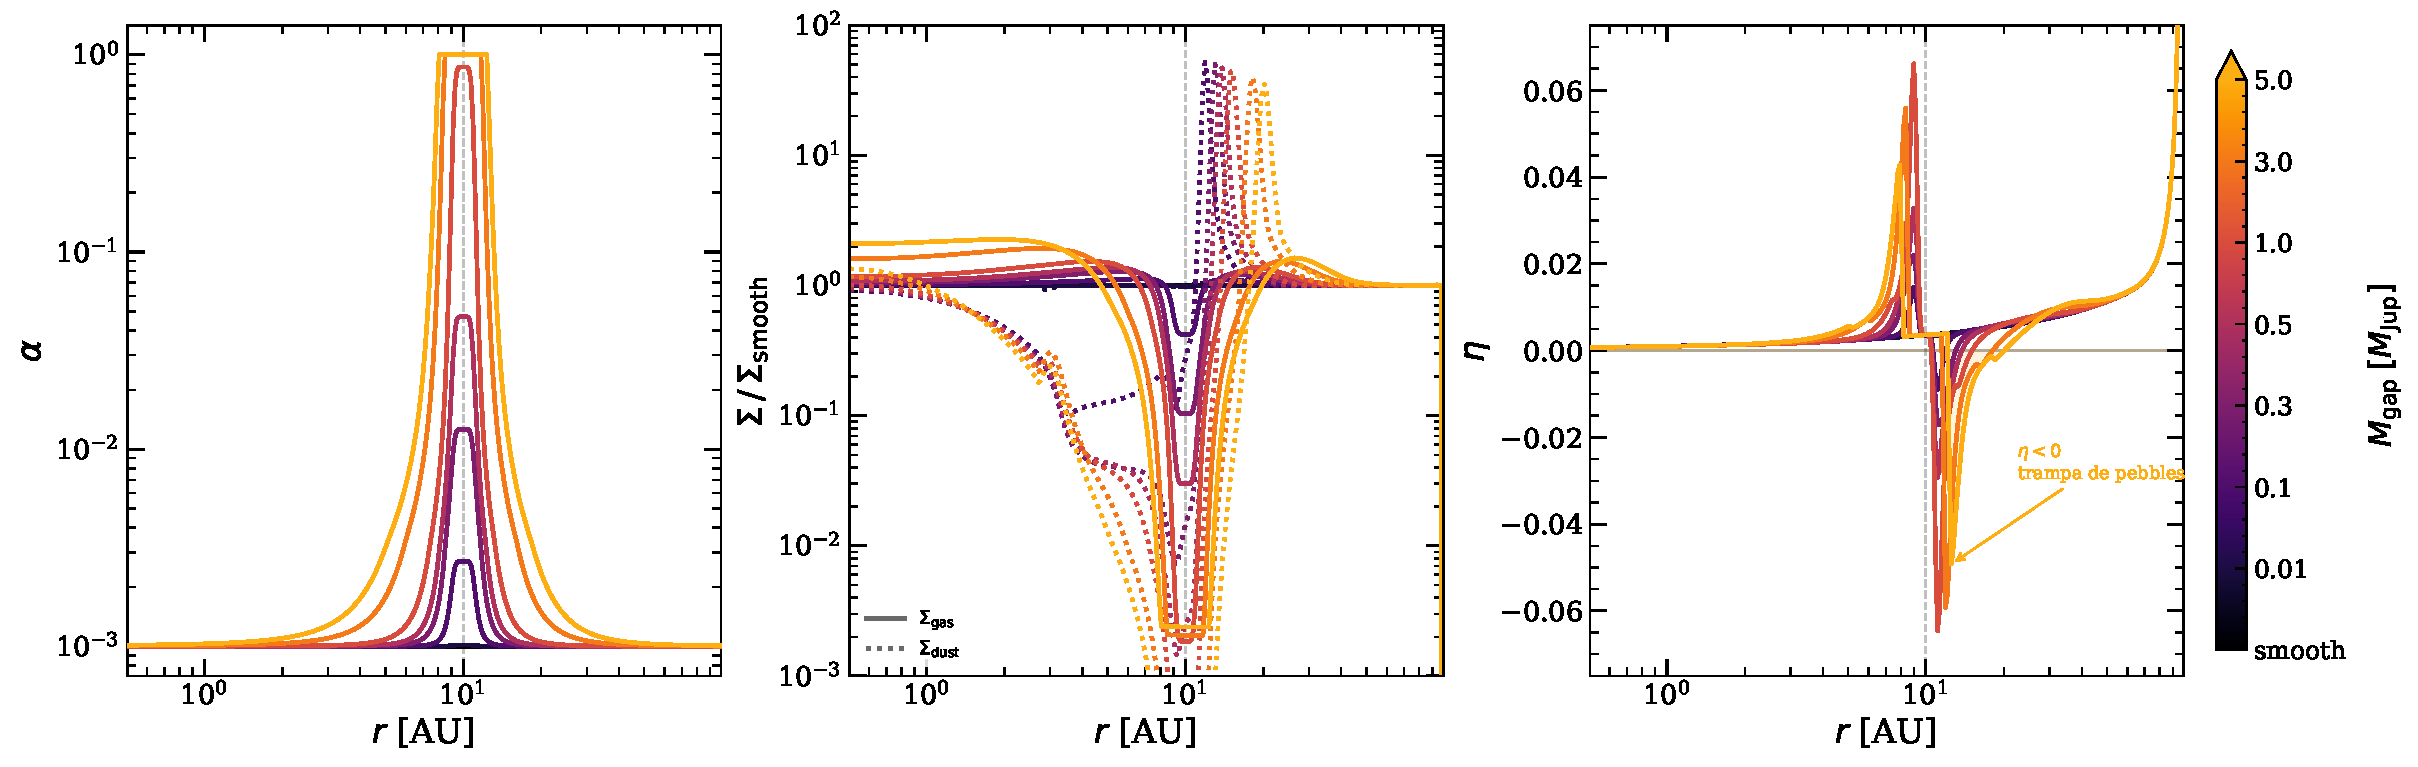
\includegraphics[width=1\linewidth]{figures/duffell_effect_panel.pdf}
    \caption{Perfiles radiales generados por la apertura de un \textit{gap} planetario según la parametrización de \citet{Duffell2020} para un valor base de $\alpha = 0.001$ e inyectando planetas con masas desde $M_{\text{gap}} = 0.01\,M_{\text{Jup}}$ hasta $5.0\,M_{\text{Jup}}$ (además del caso \textit{smooth} de control). \textbf{Panel izquierdo:} Perfil de la perturbación local aplicada sobre el parámetro de viscosidad turbulenta $\alpha(r)$. \textbf{Panel central:} Respuesta auto-consistente de la densidad superficial de gas ($\Sigma_{\text{gas}}$, líneas continuas) y polvo ($\Sigma_{\text{dust}}$, líneas punteadas) normalizadas respecto al perfil suave ($\Sigma/\Sigma_{\text{smooth}}$). \textbf{Panel derecho:} Modificación del parámetro $\eta(r)$; el cruce hacia valores negativos ($\eta < 0$) explicita la formación de la trampa de \textit{pebbles} en el borde externo de la subestructura.}
    \label{fig:duffel_efect_panel}
\end{figure}



Además, en \texttt{TriPoDPy} el parámetro $\alpha$ controla tanto la mezcla vertical y radial como las velocidades relativas entre partículas. En consecuencia, regiones menos turbulentas presentan velocidades de colisión más bajas, favoreciendo el crecimiento de partículas de mayor tamaño y números de Stokes más elevados.


% ---------------------------------------------------------
% Snowline dinámica
% ---------------------------------------------------------

\section{Evolución Dinámica de la Snowline}
\label{sec:snowline}

La línea de nieve del agua (\textit{water snowline}) corresponde a la región del disco protoplanetario donde la temperatura desciende por debajo de $\sim150-170,\mathrm{K}$, permitiendo la condensación del vapor de agua y la formación de mantos de hielo sobre las partículas sólidas \citep{Oka2011, Banzatti2023}. Esta transición modifica tanto las propiedades físicas del polvo como la composición de los pebbles disponibles para acreción planetaria \cite{}.

\invisiblesubsection{Evolución Temporal de la Tasa de Acreción}

A medida que el disco evoluciona, la disminución de la tasa de acreción estelar reduce el calentamiento viscoso y produce un enfriamiento progresivo del disco. Para describir esta evolución se adoptó una parametrización semianalítica basada en la ley de decrecimiento propuesta por \citet{Hartmann1998}, combinada con los modelos radiativos de \citet{Oka2011}. De acuerdo con \citet{Hartmann1998}, la tasa de acreción en estrellas de pre-secuencia principal decrece aproximadamente como

\begin{equation}
\dot{M}_\star \propto t^{-\eta}
\end{equation}

donde se adoptó un índice $\eta=1.5$. Asimismo, se utilizó como condición de referencia una tasa de acreción típica de $\dot{M}_\star \approx 10^{-8}M_\odot \mathrm{yr^{-1}}$ a una edad de $1\mathrm{Myr}$, característica de sistemas tipo T-Tauri. Esta parametrización permitió reconstruir la evolución temporal de la tasa de acreción a lo largo de varios millones de años (Figura~\ref{fig:hartmann_mdot}).

\begin{figure}[H]
    \centering
    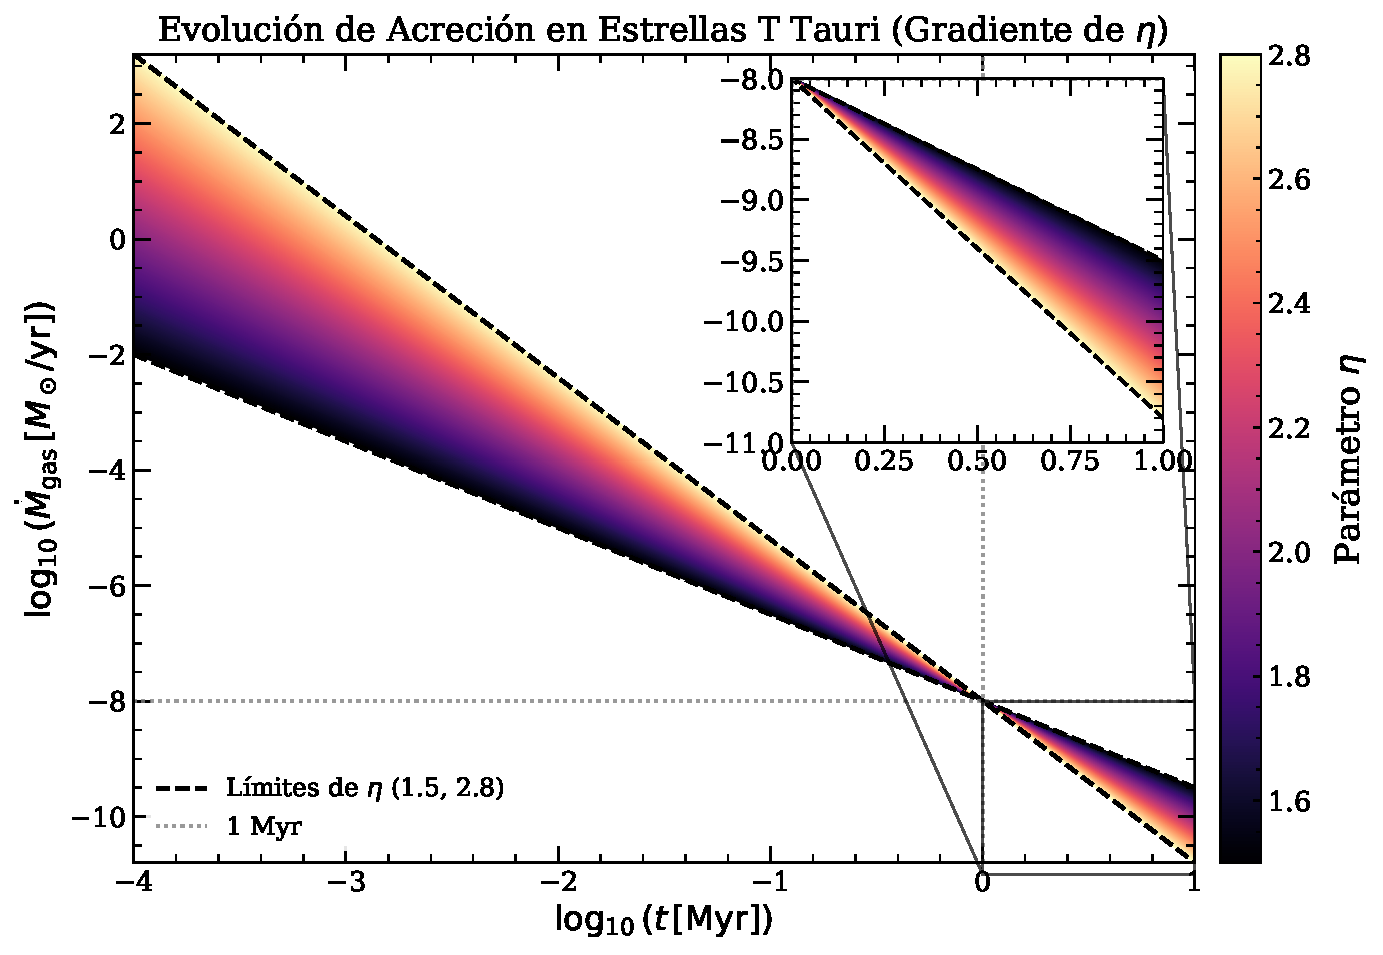
\includegraphics[width=0.8\textwidth]{figures/hartmann_mdot_gradient.pdf}
    \caption{Evoluci\'on param\'etrica de la tasa de acreci\'on de gas ($\dot{M}_{\text{gas}}$) en funci\'on del tiempo para estrellas T Tauri, basada en el modelo anal\'itico de \citet{Hartmann1998}. El eje vertical representa el logaritmo de la tasa de acreci\'on en $M_{\odot}\,\text{yr}^{-1}$, y el eje horizontal el logaritmo del tiempo en Myr. La regi\'on sombreada ilustra una familia de soluciones donde la barra de color indica el valor del exponente de decaimiento $\eta$, variando continuamente desde $1.5$ (tonos oscuros) hasta $2.8$ (tonos claros). Las l\'ineas discontinuas negras delimitan las cotas superior e inferior correspondientes a estos valores extremos de $\eta$. Se incluye una l\'inea punteada de referencia marcando el tiempo $t = 1\text{ Myr}$ ($\log_{10} t = 0$). El recuadro interior (\textit{inset}) muestra una vista ampliada de la etapa de evoluci\'on tard\'ia ($t \geq 1\text{ Myr}$), destacando la divergencia en la ca\'ida de la tasa de acreci\'on dependiente del par\'ametro $\eta$.}
    \label{fig:hartmann_mdot}
\end{figure}

Los valores temporales de la tasa de acreción se combinaron con los perfiles de temperatura y posición de la snowline obtenidos por \citet{Oka2011} (Figura~\ref{fig:dynamic_snowline}). A partir de esta información se construyó una parametrización de la evolución temporal de $R_{\rm snow}(t)$ mediante interpolación, permitiendo describir la migración de la línea de nieve a lo largo de la evolución del disco.

Para las etapas más tempranas ($t \lesssim 0.2,\mathrm{Myr}$), correspondientes a tasas de acreción elevadas ($\dot{M}_{gas} \gtrsim 10^{-7},M\odot,\mathrm{yr}^{-1}$), los valores se encuentran fuera del rango cubierto por los modelos de \citet{Oka2011}. En consecuencia, se asumió que la línea de nieve permanecía aproximadamente constante en $R_{\rm snow}\simeq2.7,\mathrm{AU}$ hasta que la disminución de la tasa de acreción permitió el inicio de su migración hacia el interior del disco.


\begin{figure}[H]
    \centering
    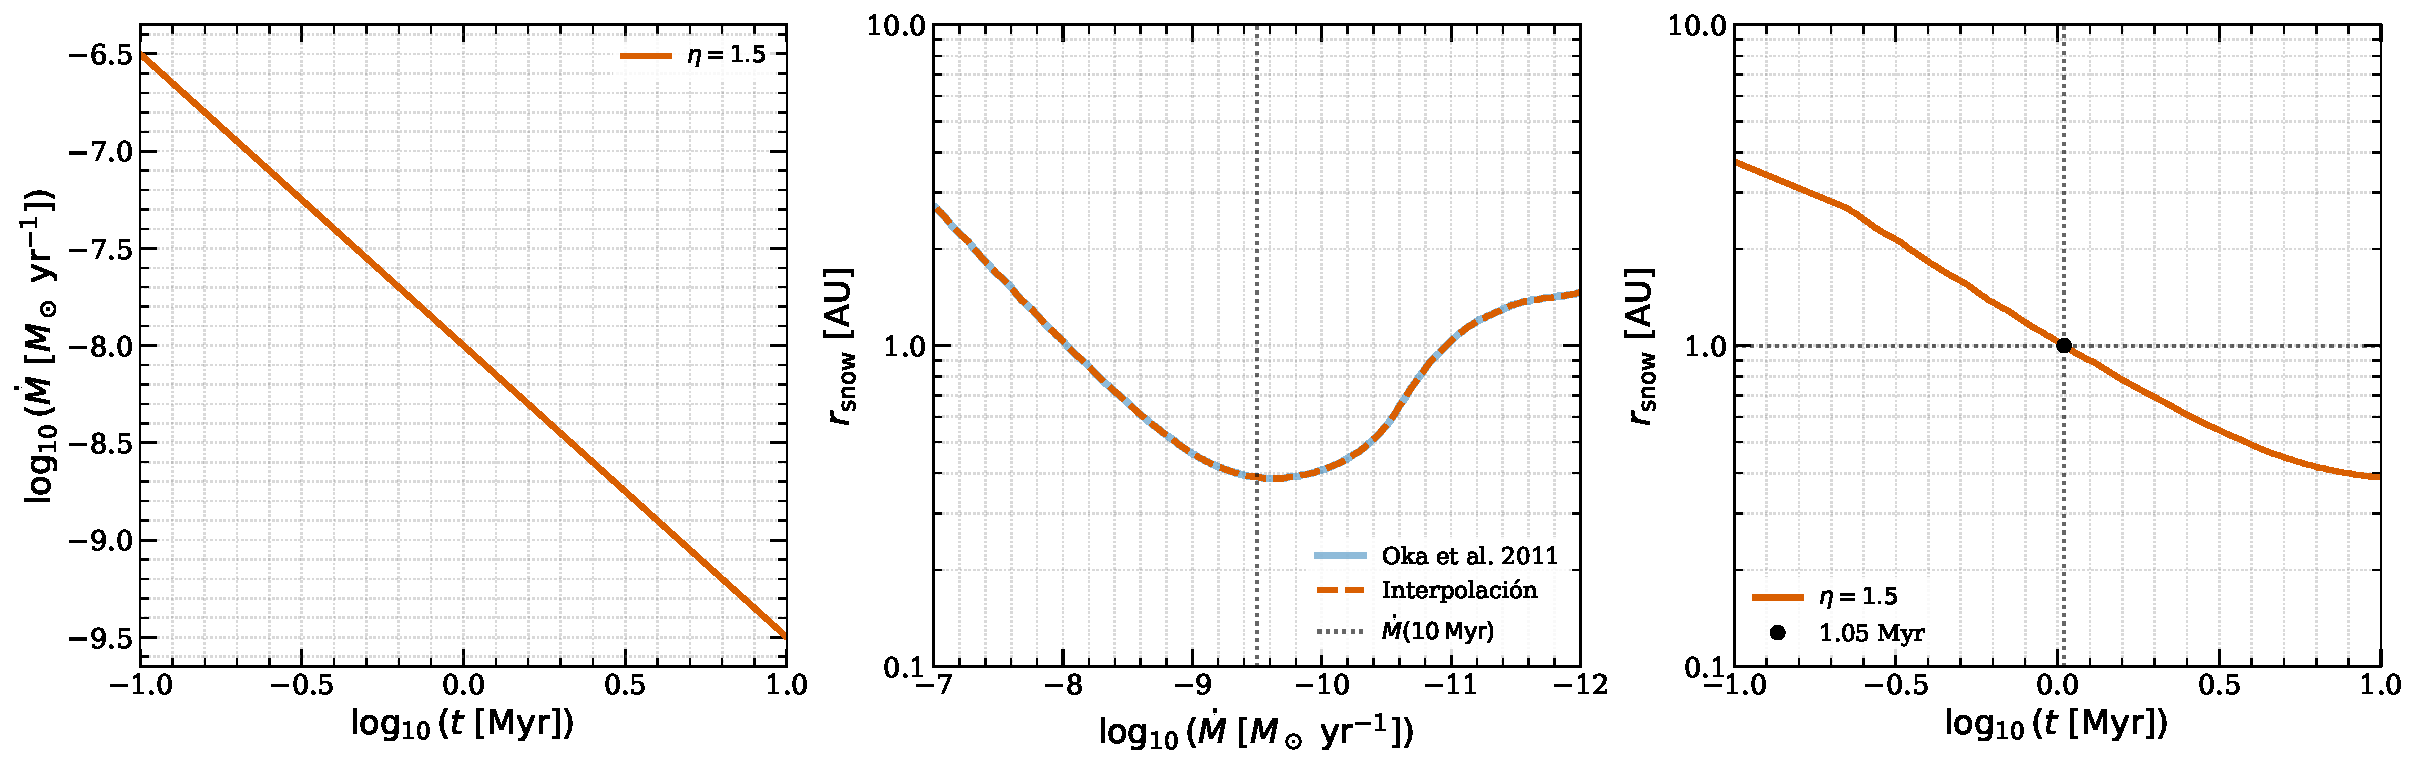
\includegraphics[width=1\textwidth]{figures/dynamic_snowline_oka_interpolation.pdf}
    \caption{Evoluci\'on din\'amica de la posici\'on de la l\'inea de nieve (\textit{snowline}) en la simulaci\'on base. 
    \textbf{Panel izquierdo:} Decaimiento temporal de la tasa de acreci\'on de gas ($\dot{M}$) asumiendo un modelo param\'etrico con exponente $\eta = 1.5$ \citep{Hartmann1998}. 
    \textbf{Panel central:} Dependencia te\'orica del radio de la \textit{snowline} ($r_{\text{snow}}$) respecto a la tasa de acreci\'on. Se muestra el modelo anal\'itico de \citet{Oka2011} (l\'inea s\'olida celeste) junto con la interpolaci\'on aplicada en este trabajo (l\'inea discontinua naranja). El eje horizontal ($\log_{10}\dot{M}$) se ha invertido intencionalmente para que la evoluci\'on temporal fluya hacia la derecha. La l\'inea vertical punteada sirve de referencia para la tasa de acreci\'on a los $10\text{ Myr}$. 
    \textbf{Panel derecho:} Trayectoria final de la \textit{snowline} acoplando las dos relaciones anteriores en funci\'on del tiempo astrof\'isico. El marcador negro y las l\'ineas punteadas transversales resaltan el momento exacto en el que la \textit{snowline} retrocede cruzando la marca de $1.0\text{ AU}$, lo cual ocurre a los $1.05\text{ Myr}$.}
    \label{fig:dynamic_snowline}
\end{figure}

\invisiblesubsection{Fragmentación Dependiente de la Composición Hielo-Roca}

La velocidad de fragmentación $v_{\rm frag}$ constituye uno de los parámetros más importantes en la evolución del polvo, ya que determina el tamaño máximo alcanzado por los pebbles y, en consecuencia, controla tanto sus velocidades de deriva radial como la eficiencia del transporte de sólidos. En este trabajo se adoptó una parametrización dependiente de la posición de la \textit{snowline}, implementada mediante una función escalón:
\begin{equation} v_{\rm frag}(r,t) = \begin{cases} 10 \, \text{m/s} & \text{si } r \geq R_{\rm snow}(t) \quad \text{(Material pegajoso rico en hielos)} \\ 1 \, \text{m/s} & \text{si } r < R_{\rm snow}(t) \quad \text{(Matriz rígida seca de silicatos)} \end{cases} \end{equation}
donde los valores exteriores representan agregados ricos en hielo y los interiores corresponden a partículas dominadas por silicatos. Esta prescripción se basa en experimentos de laboratorio que muestran que la presencia de hielo aumenta significativamente la resistencia a la fragmentación, permitiendo velocidades críticas del orden de \SI{10}{\meter\per\second}

Si bien estudios más recientes sugieren que la resistencia mecánica del hielo puede disminuir a temperaturas muy bajas, alcanzando valores comparables a los de los silicatos
(\SIrange{1}{3}{\meter\per\second}) \citep{Musiolik_Grzegorz_Gerhard2019}, en esta tesis se adoptó la aproximación estándar utilizada en modelos de evolución de polvo y formación planetaria. Bajo esta prescripción, valores elevados de $v_{\rm frag}$ favorecen la formación de pebbles de mayor tamaño, los cuales experimentan una deriva radial más eficiente y pueden modificar significativamente el flujo de sólidos hacia las regiones internas del disco.


% ---------------------------------------------------------
% Pebble Accretion
% ---------------------------------------------------------
\section{Modelo Computacional de Acreción: \texttt{PA3Py}}
\label{sec: PA3Py}

\texttt{PA3Py}\footnote{El código fuente completo de PA3Py, incluyendo 
documentación y tutoriales, está disponible públicamente en: 
\url{https://github.com/maximiliano-valderrama/pa3py}. El repositorio 
incluye además los datos de las 5006 trayectorias simuladas, scripts 
de análisis y figuras suplementarias para robustez a variaciones en 
$M_{\rm emb,0}$.} es el módulo de postprocesado desarrollado en este trabajo para estudiar el crecimiento de embriones planetarios mediante pebble accretion. El código implementa numéricamente las ecuaciones descritas en la Sección~\ref{sec:pebble_accretion} del Capítulo~\ref{cap:marco_teorico}, incluyendo los distintos regímenes de acreción (2D y 3D), así como las masas características asociadas al inicio de la acreción y al aislamiento por pebbles.

La evolución temporal se calcula mediante un esquema explícito de Euler utilizando como entrada los \textit{snapshots} en formato HDF5 generados por \texttt{TriPoDPy}. Para cada instante, el código extrae las propiedades locales del disco, incluyendo la densidad superficial del gas y del polvo, la temperatura, la altura de escala y las distribuciones de tamaño representadas por las poblaciones características ($a_0$, $a_1$ y $a_{\rm max}$).

\invisiblesubsection{Regímenes de Acreción}

Durante la integración, se introducen embriones planetarios de masa inicial $M_c$ en radios orbitales prefijados y se calcula su crecimiento siguiendo la formulación presentada por \citet{Ormel2017} y \citet{Drazkowska2023}. En primer lugar, se verifica que la masa del embrión supere la masa mínima necesaria para que la acreción de pebbles sea eficiente, conocida como \textit{onset mass},

\begin{equation}
M_{\rm PA,onset}=St\text{ }\eta^3\text{ }M_\star 
\end{equation}

donde $St$ es el número de Stokes y $\eta$ cuantifica la desviación sub-Kepleriana del gas. Para masas inferiores a este umbral, el crecimiento está dominado por colisiones geométricas y resulta poco eficiente.

Una vez superada esta condición, la acreción se calcula utilizando las expresiones correspondientes a los regímenes bidimensionales dominados por \textit{headwind} o (\textit{shear}), de acuerdo con las ecuaciones presentadas por \citet[][Ecs. 7.9 y 7.13]{Ormel2017}.

\invisiblesubsection{Corrección por Espesor Vertical}

En regiones donde la altura de la capa de pebbles excede el radio efectivo de captura gravitacional, el crecimiento se reduce mediante la corrección de transición suave propuesta por \citet[][Ec. 7.24]{Ormel2017}. Este factor permite describir la transición entre los regímenes 2D y 3D y tiene en cuenta la distribución vertical del polvo en el disco.

\invisiblesubsection{Masa de Aislamiento}

El crecimiento por pebble accretion se detiene cuando el planeta alcanza la masa de aislamiento,

\begin{equation}
M_{\rm iso}\approx25,M_\oplus
\left(\frac{H_{\rm gas}/r}{0.05}\right)^3
\frac{M_\star}{M_\odot},
\label{eq: Mass_isolation}
\end{equation}

siguiendo la aproximación adoptada por \citet{Lambrechts2014} y \citet{Drazkowska2023}. A esta masa, las perturbaciones gravitacionales inducidas por el planeta modifican localmente el perfil de presión del gas, generando una barrera que interrumpe el flujo radial de pebbles y detiene el crecimiento posterior mediante este mecanismo.


Una limitación del enfoque de \textit{post-procesado} radica en que \texttt{PA3Py} utiliza las propiedades del disco obtenidas por \texttt{TriPoDPy} sin retroalimentar su evolución. Por ello, la masa acrecida por un planeta no se descuenta del reservorio de sólidos disponible para otros cuerpos. Como resultado, simulaciones con múltiples planetas no incluyen la competencia por el flujo de pebbles, lo que puede producir una sobreestimación de la masa total acumulada.

\invisiblesubsection{Seguimiento Composicional del Contenido de Agua}

Para seguir la composición del material acrecido, se incorporó una contabilidad sencilla basada en la posición de origen de los pebbles respecto de la snowline. De manera consistente con trabajos previos \citep{Bitsch2021,McCloat2025}, se asumió que los pebbles formados más allá de la línea de nieve ($r \geq R_{\rm snow}(t)$) están compuestos por un 50\% de material refractario y un 50\% de hielo de agua, mientras que aquellos provenientes de regiones interiores se consideraron completamente secos. A partir de esta prescripción se calculó la evolución temporal del contenido de agua de cada planeta.


% ---------------------------------------------------------
% Resultados y Validación
% ---------------------------------------------------------
\section{Resultados y Validación de Simulaciones}

\invisiblesubsection{Configuración del Disco y Estructura Termodinámica}

Para este estudio, se generaron un total de 1323 simulaciones de disco físico bidimensionales, abarcando distintas configuraciones de subestructuras. Estas incluyen discos de control sin perturbaciones (\textit{Smooth}, 24 casos), discos con un único \textit{gap} (759 casos) y \textit{Sinusoidal} (540 casos).

Un aspecto fundamental de estas simulaciones es la suposición de un perfil térmico estático. Dado que la altura de escala de presión del gas obedece la proporcionalidad matemática
\begin{equation}
\frac{H_p}{r} \propto T^{1/2} r^{1/2} M_\star^{-1/2},
\end{equation}
y considerando que la masa estelar se asume constante en $1\,M_\odot$, el perfil de temperatura impuesto fija una estructura termodinámica invariante para el gas de fondo. El análisis de las simulaciones confirmó empíricamente que a $1\,{\rm AU}$, la razón de aspecto del disco gaseoso resulta idéntica en todas las simulaciones, arrojando un valor de $H_p/r \simeq 0.027$. 

Esta constancia termodinámica tiene implicaciones directas sobre el crecimiento de los núcleos. Recordando la expresión teórica para la masa de aislamiento inducida por el flujo de \textit{pebbles} \eqref{eq: Mass_isolation} y evaluando con el valor derivado de $H_p/r \simeq 0.027$, se obtiene una masa máxima teórica de $M_{\rm iso} \simeq 3.96\,M_\oplus$ a $1\,{\rm AU}$. Por lo tanto, la estructura del gas actúa como un escenario estático que impone una cota de masa al crecimiento de los embriones.

\invisiblesubsection{Inyección de Embriones}

Sobre esta colección de 1323 simulaciones de discos, se realizó un barrido exhaustivo del espacio de parámetros inyectando embriones planetarios con cuatro masas iniciales distintas: $M_{\rm emb,0} = 10^{-5},\; 10^{-4},\; 10^{-3},\; 10^{-2}\,M_\oplus$. Este procedimiento arrojó un catálogo total de 5292 trayectorias evolutivas planetarias únicas.

Con el fin de garantizar la consistencia numérica de la muestra, se aplicó un procedimiento de control de calidad sobre las 5292 trayectorias. Se definieron dos criterios principales de exclusión:

\begin{itemize}
    \item \textbf{Muerte prematura:} Simulaciones que finalizaron antes de alcanzar $1\,{\rm Myr}$ sin acumular al menos el $90\%$ de la masa de aislamiento esperada.
    \item \textbf{Inestabilidad numérica:} Integraciones que presentaron variaciones abruptas de masa en los últimos pasos temporales ($R_{\rm var} \geq 10\%$).
\end{itemize}

La aplicación de estos criterios condujo a la eliminación de aproximadamente 286 simulaciones ($\approx 5.4\%$ de la muestra), equivalente a $\sim 71$ casos por cada valor de $M_{\rm emb,0}$. Tras esta depuración, se obtuvo una muestra final de 5006 trayectorias válidas, empleadas en todos los análisis posteriores.


=========================================================% CAPÍTULO 4 — RESULTADOS Y ANÁLISIS% =========================================================

\chapter{Resultados y Análisis}
\label{cap}

% =========================================================
\section{Evolución del polvo}
\label{sec:Evolución_de_polvo}
% =========================================================

Esta sección analiza cómo la evolución del polvo responde a tres parámetros físicos
que controlan el transporte de sólidos en discos protoplanetarios estructurados:
la velocidad de fragmentación $v_{\rm frag}$, la intensidad de las perturbaciones
de presión y el nivel de turbulencia parametrizado mediante $\alpha$. La evolución
se estudia a partir de diagramas de Hovmöller de la relación polvo-gas
$\Sigma_d/\Sigma_g$, comparando discos suaves con discos que contienen una única
trampa de presión o una estructura sinusoidal de múltiples anillos.

% =========================================================
\invisiblesubsection{Impacto de la Velocidad de Fragmentación}
% =========================================================

La Figura~\ref{fig:hovmoller_vfrag} muestra la evolución espacio-temporal de
$\Sigma_d/\Sigma_g$ para tres velocidades de fragmentación
($v_{\rm frag}=1,\;3,\;10\,{\rm m\,s^{-1}}$), manteniendo fijo
$\alpha=10^{-3}$ y considerando tres arquitecturas del disco:
suave, gap único y perfil sinusoidal.

\begin{figure}[h!]
    \centering
    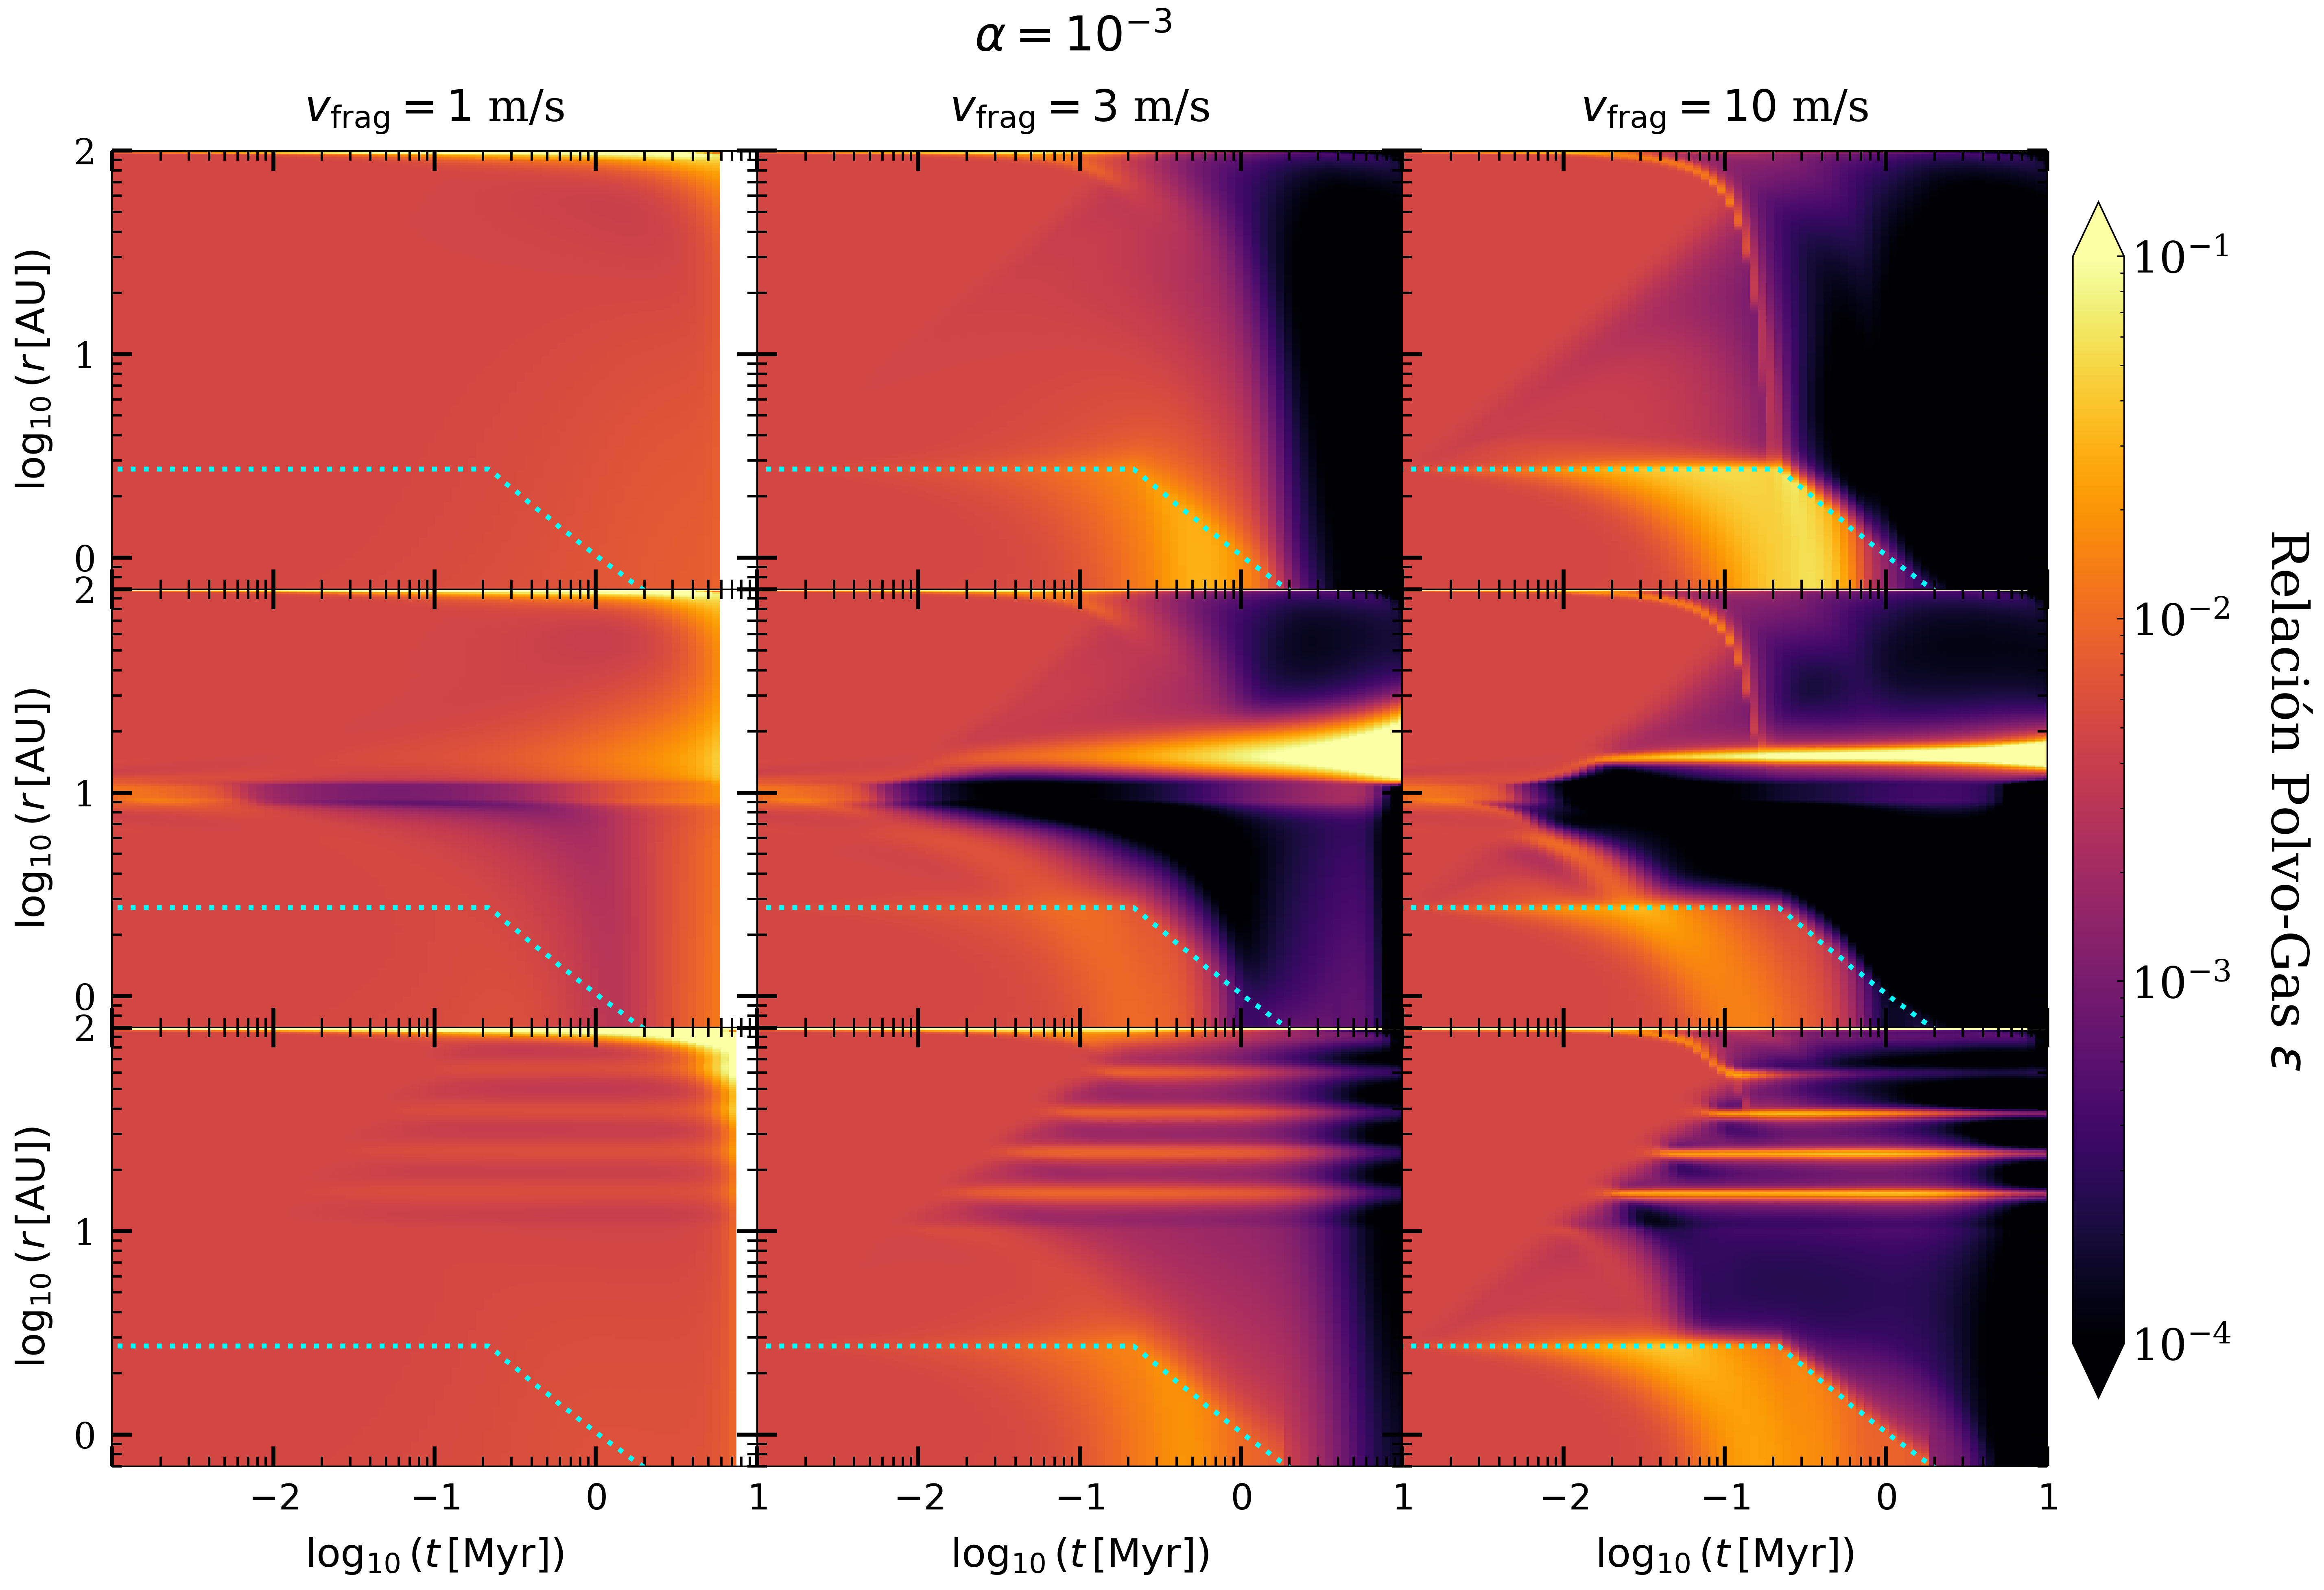
\includegraphics[width=\textwidth]{figures/4_fig_resultados/figura1_vfrags.png}
    \caption{Diagramas de Hovmöller de $\Sigma_d/\Sigma_g$ para
    $v_{\rm frag}=1,\;3,\;10\,{\rm m\,s^{-1}}$ (columnas) y tres arquitecturas
    del disco (filas): disco suave, gap único y perfil sinusoidal.
    La línea cian punteada indica la posición temporal del snowline.}
    \label{fig:hovmoller_vfrag}
\end{figure}

En el disco suave, la distribución de polvo evoluciona de manera similar para los
tres valores de $v_{\rm frag}$. La relación polvo-gas disminuye progresivamente
hacia radios pequeños debido a la deriva radial, sin observarse acumulaciones
locales persistentes. En ausencia de máximos de presión, modificar la velocidad
de fragmentación tiene un efecto reducido sobre la distribución global del polvo.

La situación cambia al introducir subestructuras. Tanto en el disco con un único
gap como en el perfil sinusoidal, el incremento de $v_{\rm frag}$ favorece la
formación de anillos con mayor relación polvo-gas. Para
$v_{\rm frag}=1\,{\rm m\,s^{-1}}$ la acumulación es prácticamente inexistente,
mientras que para $v_{\rm frag}=10\,{\rm m\,s^{-1}}$ aparecen reservorios sólidos
bien definidos en los máximos locales de presión.

Cuando el snowline alcanza estas regiones de acumulación
($t\sim1\,{\rm Myr}$), el comportamiento también depende de
$v_{\rm frag}$. En el caso de alta velocidad de fragmentación se observa la
liberación del material previamente retenido, visible como un aumento transitorio
de $\Sigma_d/\Sigma_g$ en el disco interior. Este fenómeno no aparece de forma
apreciable para $v_{\rm frag}=1\,{\rm m\,s^{-1}}$, donde la ausencia de un
reservorio sólido impide un transporte posterior de material hacia radios menores.

En conjunto, estos resultados muestran que el efecto de $v_{\rm frag}$ se manifiesta
principalmente cuando existen trampas de presión capaces de almacenar material.
En discos sin subestructuras, la evolución continúa dominada por la deriva radial.

% =========================================================
\invisiblesubsection{Dependencia con la Amplitud de la Perturbación}
% =========================================================

La Figura~\ref{fig:hovmoller_arquitectura} muestra la evolución del polvo al variar
la intensidad de la perturbación, representada por la masa del planeta que abre el
gap o por la amplitud del perfil sinusoidal, manteniendo
$v_{\rm frag}=10\,{\rm m\,s^{-1}}$ y $\alpha=10^{-3}$.

\begin{figure}[H]
    \centering
    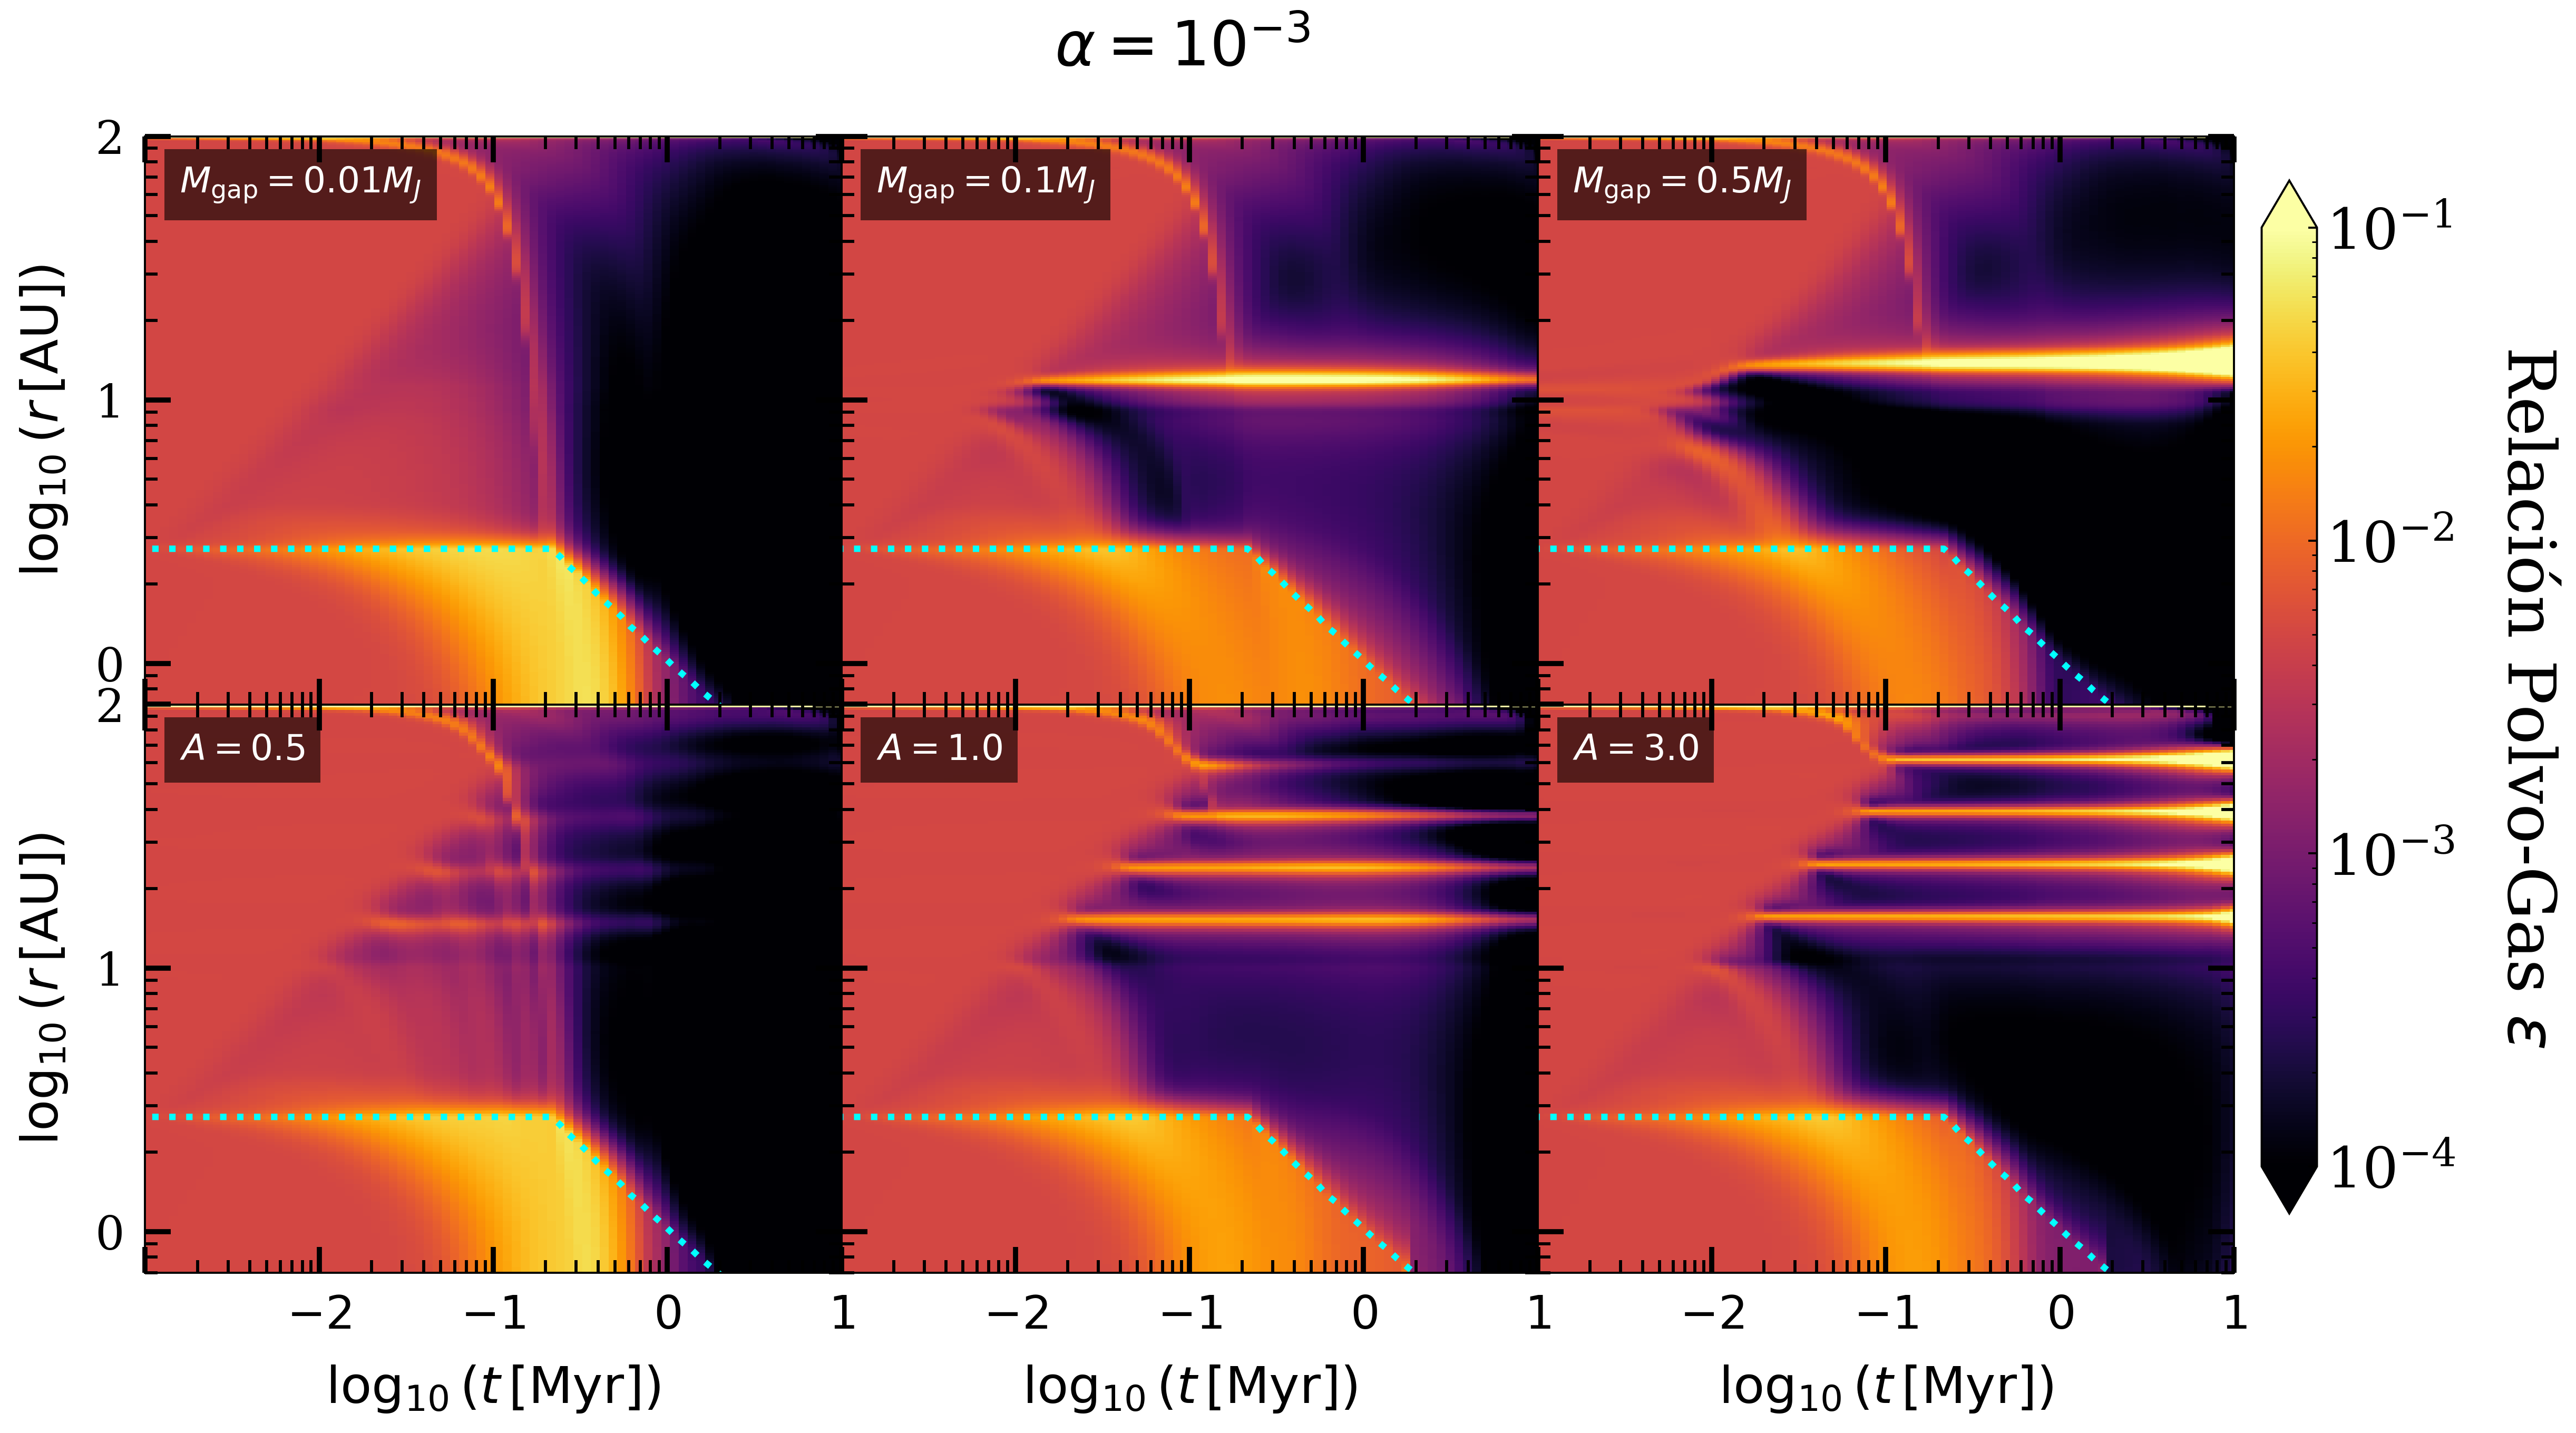
\includegraphics[width=1\textwidth]{figures/4_fig_resultados/figura2_masas.png}
    \caption{Diagramas de Hovmöller variando la amplitud de la perturbación para
    $v_{\rm frag}=10\,{\rm m\,s^{-1}}$ y $\alpha=10^{-3}$.}
    \label{fig:hovmoller_arquitectura}
\end{figure}

Para perturbaciones débiles
($M_{\rm gap}=0.01\,M_{\rm Jup}$ o $A=0.5$), la estructura de presión resulta
insuficiente para generar una acumulación significativa de sólidos. La relación
polvo-gas permanece cercana a la del disco suave durante toda la evolución.

Al aumentar la amplitud de la perturbación
($M_{\rm gap}=0.1\,M_{\rm Jup}$ o $A=1.0$), se desarrolla un anillo bien definido
con relaciones polvo-gas del orden de $10^{-2}$--$10^{-1}$. Cuando el snowline
atraviesa esta región, parte del material retenido es transportado nuevamente hacia
el disco interior, produciendo un episodio transitorio de enriquecimiento en polvo.

En el régimen de perturbaciones más intensas
($M_{\rm gap}=0.5\,M_{\rm Jup}$ o $A=3.0$), la acumulación inicial es aún mayor,
pero el reservorio permanece estable durante el resto de la evolución. Incluso
después del cruce del snowline, la mayor parte del material continúa retenida en
el borde exterior de la trampa, manteniendo empobrecidas las regiones interiores.

En conjunto, estos resultados muestran que la eficiencia del atrapamiento de polvo depende de manera no monótona de la intensidad de la perturbación. Mientras perturbaciones débiles no generan reservorios significativos, perturbaciones excesivamente profundas retienen el material durante toda la evolución del disco, limitando su liberación posterior hacia las regiones internas.

% =========================================================
\invisiblesubsection{Efecto de la Turbulencia}
% =========================================================

La Figura~\ref{fig:hovmoller_turbulencia} presenta la evolución del polvo para
$\alpha=10^{-4}$, $5\times10^{-4}$ y $10^{-3}$, utilizando
$v_{\rm frag}=10\,{\rm m\,s^{-1}}$ y la configuración de perturbación que produce
la acumulación más eficiente en la sección anterior.

\begin{figure}[H]
    \centering
    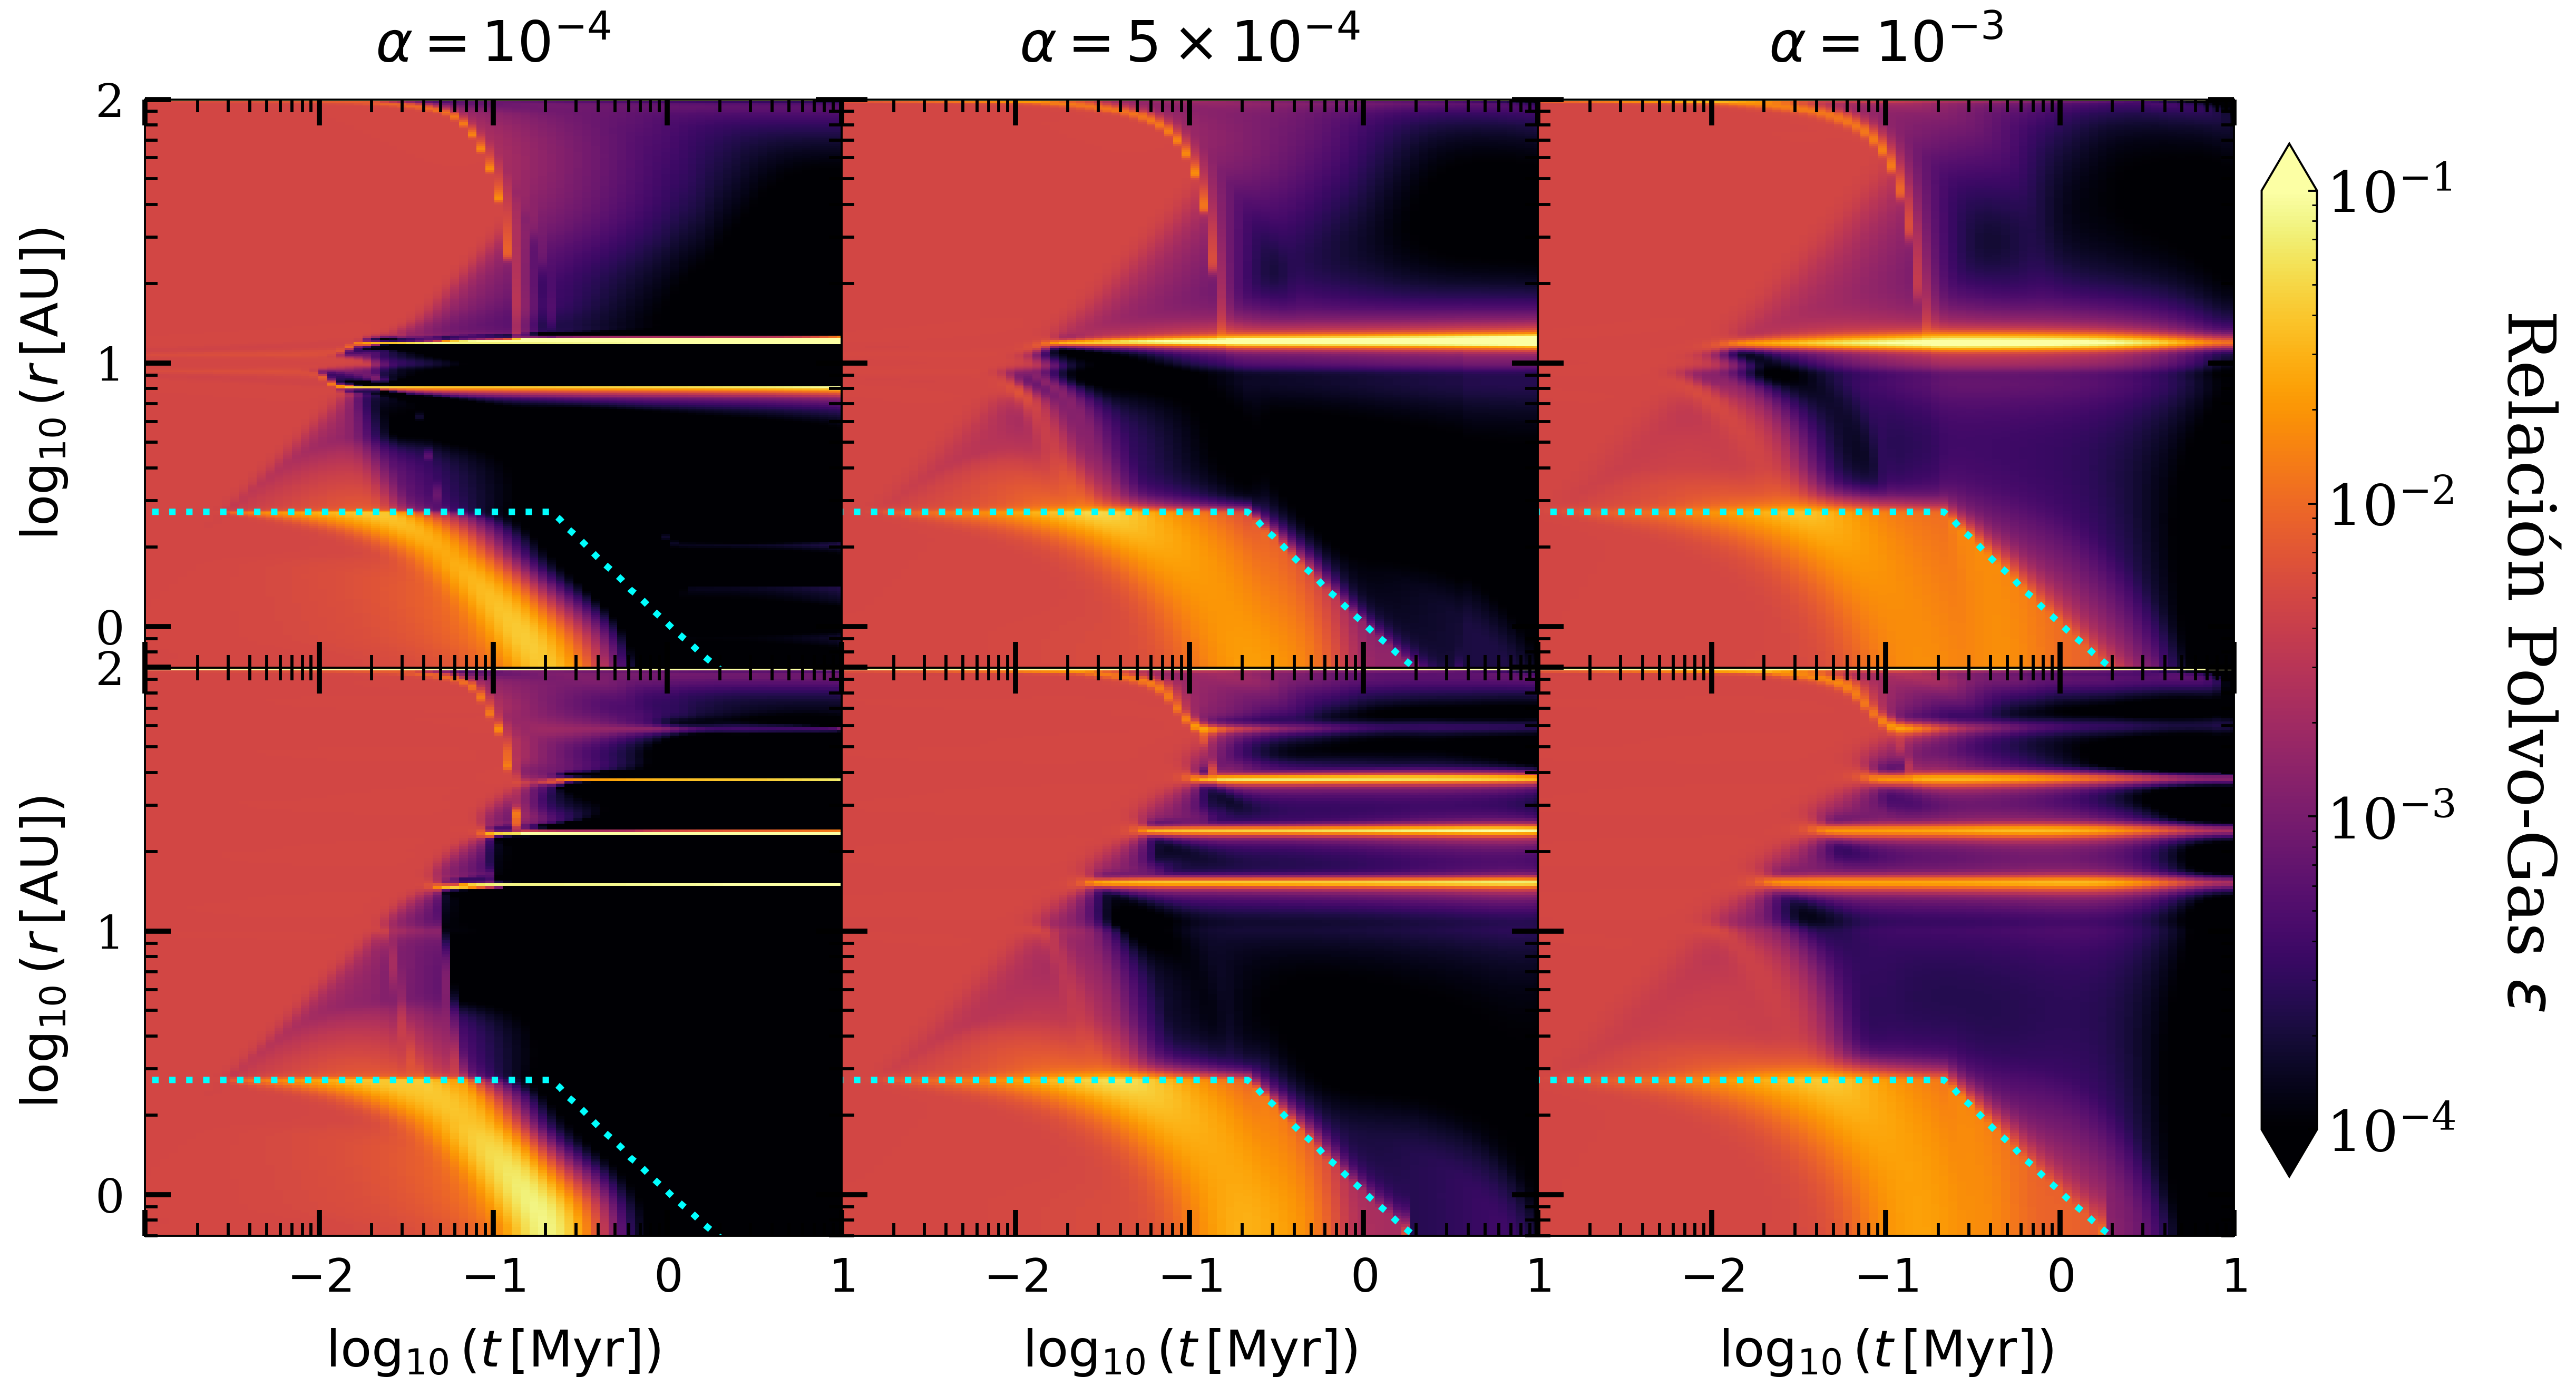
\includegraphics[width=\textwidth]{figures/4_fig_resultados/figura3_turbulencia.png}
    \caption{Diagramas de Hovmöller variando el parámetro turbulento $\alpha$.}
    \label{fig:hovmoller_turbulencia}
\end{figure}

Para $\alpha=10^{-4}$ se desarrollan anillos estrechos y con elevada concentración
de polvo, alcanzando relaciones $\Sigma_d/\Sigma_g$ cercanas a $10^{-1}$ tanto en
la configuración con gap como en el perfil sinusoidal.

Al incrementar la turbulencia hasta
$\alpha=5\times10^{-4}$, los anillos permanecen visibles, aunque presentan una
disminución apreciable de la concentración máxima y una distribución radial más
extendida.

Finalmente, para $\alpha=10^{-3}$ la acumulación de polvo se reduce de manera
importante. Los anillos se vuelven difusos y la distribución de sólidos tiende a
ser más uniforme, disminuyendo la cantidad de material retenido en las trampas de
presión.

En consecuencia, dentro del rango de parámetros explorado, la turbulencia actúa
como un mecanismo que reduce la eficiencia del atrapamiento de polvo, limitando la
formación de reservorios sólidos de alta densidad superficial.

% =========================================================
\section{Crecimiento planetario}
\label{sec:crecimiento_individual}
% =========================================================

En esta sección se analiza la evolución temporal de la masa de un embrión planetario situado a $1\,{\rm AU}$, con una masa inicial
$M_{\rm emb,0}=10^{-4}\,M_\oplus$. El crecimiento se presenta para distintas configuraciones del disco con el objetivo de evaluar la influencia de la velocidad de fragmentación, la arquitectura de las subestructuras y el nivel de turbulencia sobre la masa final alcanzada por el embrión.

Como referencia, se indican el umbral de $0.1\,M_\oplus$, utilizado para identificar los casos que alcanzan masas planetarias, y la masa de aislamiento local $M_{\rm iso}$.

\begin{figure}[h!]
    \centering
    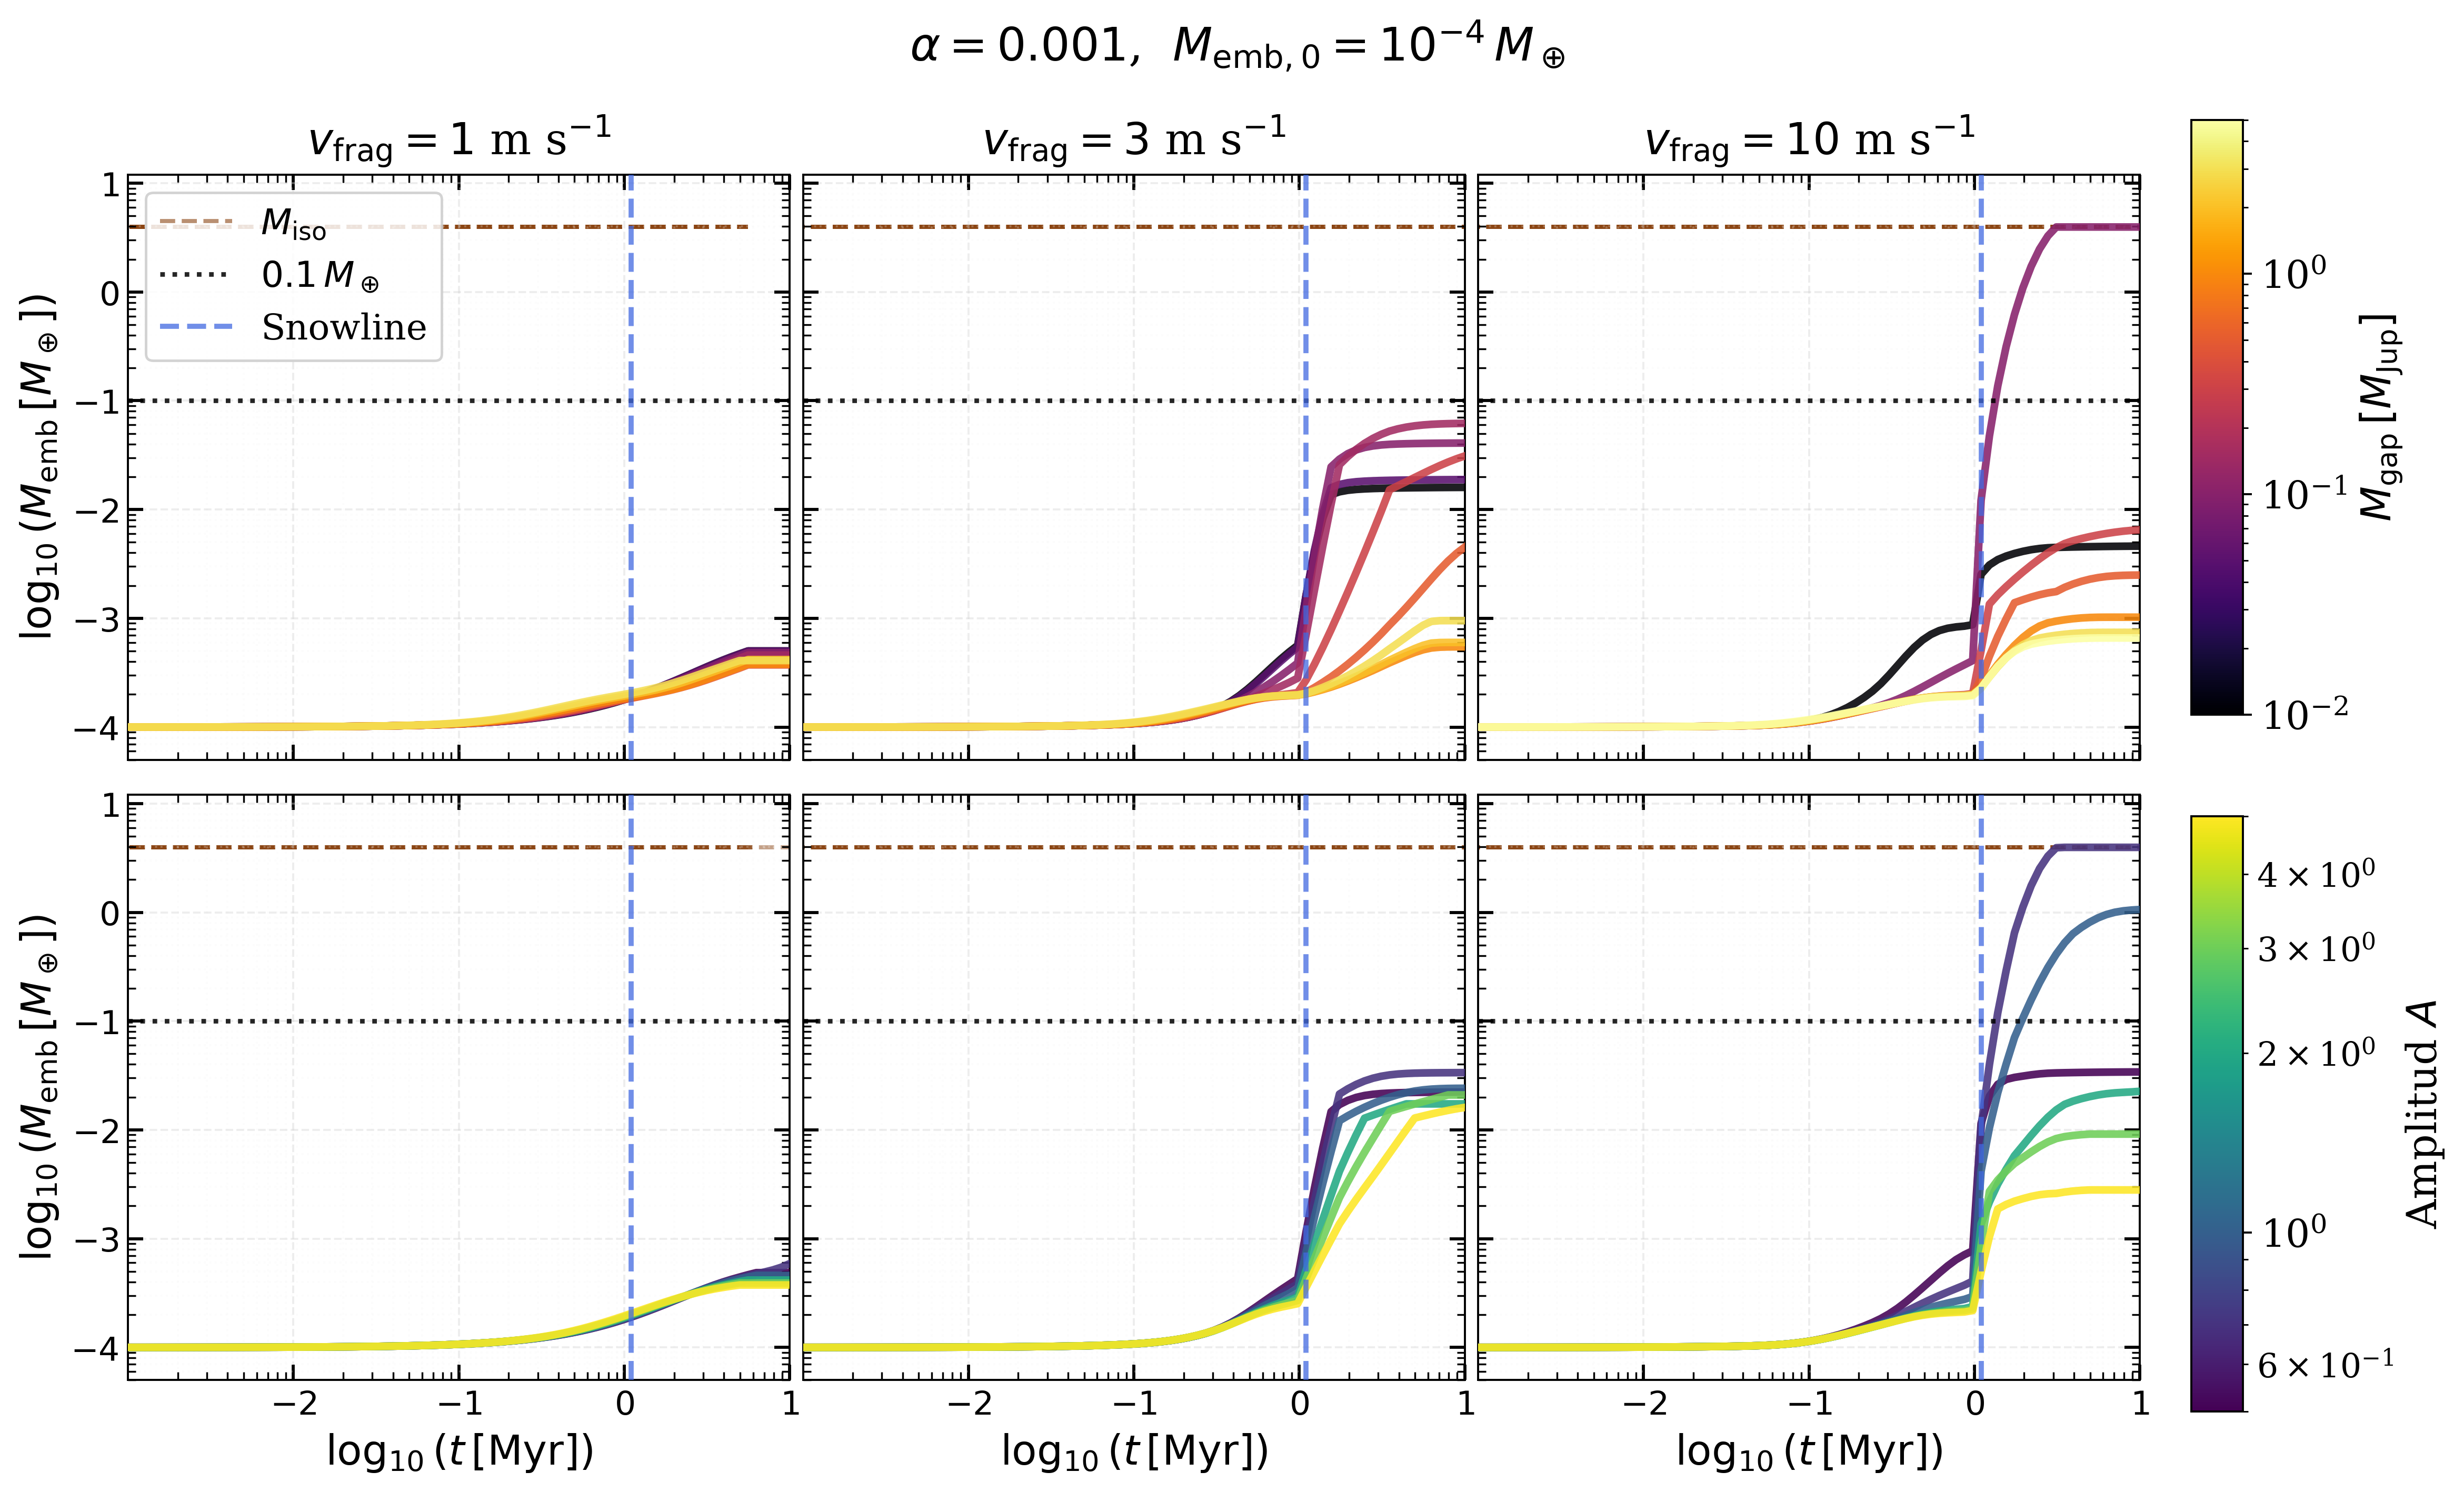
\includegraphics[width=1\textwidth]{figures/4_fig_resultados/figura_A3_gap_sinusoidal.png}
    \caption{
    Evolución temporal de la masa de un embrión situado a $1\,{\rm AU}$ para distintas velocidades de fragmentación (columnas) y configuraciones de subestructuras (filas). En la fila superior, el color representa la masa del planeta que abre un único gap; en la inferior, la amplitud de un perfil sinusoidal de viscosidad. Se adopta $\alpha=10^{-3}$ y $M_{\rm emb,0}=10^{-4}\,M_\oplus$. La línea vertical azul indica el cruce de la snowline, mientras que las líneas horizontales muestran el umbral de $0.1\,M_\oplus$ y la masa de aislamiento $M_{\rm iso}$. Se observa que el crecimiento más eficiente ocurre para valores intermedios de la intensidad de la perturbación.
}
    \label{fig:gap_sinusoidal}
\end{figure}

% =========================================================
\invisiblesubsection{Gap único}
% =========================================================

La fila superior de la Figura~\ref{fig:gap_sinusoidal} muestra la evolución temporal de la masa del embrión para un disco con un único gap localizado en $10\,{\rm AU}$, utilizando $\alpha=10^{-3}$ y una masa inicial
$M_{\rm emb,0}=10^{-4}\,M_\oplus$.

Para $v_{\rm frag}=1\,{\rm m\,s^{-1}}$, todas las trayectorias muestran un crecimiento limitado durante toda la evolución y permanecen por debajo de $10^{-3}\,M_\oplus$. Al aumentar la velocidad de fragmentación hasta $3\,{\rm m\,s^{-1}}$, las trayectorias comienzan a divergir alrededor de $t\sim10^{6}$ años, aunque ninguna supera el umbral de $0.1\,M_\oplus$.

En el caso de $v_{\rm frag}=10\,{\rm m\,s^{-1}}$, varias trayectorias experimentan un incremento pronunciado de masa después de aproximadamente $10^{6}$ años. Las mayores masas finales corresponden a valores intermedios de $M_{\rm gap}$, mientras que los gaps menos profundos y los más profundos producen masas finales considerablemente menores.

% =========================================================
\invisiblesubsection{Perfil sinusoidal}
% =========================================================

La fila inferior de la Figura~\ref{fig:gap_sinusoidal} presenta el mismo experimento utilizando un perfil sinusoidal compuesto por múltiples anillos.

El comportamiento general es similar al obtenido para el caso de un único gap. Para $v_{\rm frag}=1\,{\rm m\,s^{-1}}$, el crecimiento permanece reducido en todas las configuraciones. Al considerar $v_{\rm frag}=3\,{\rm m\,s^{-1}}$, las trayectorias comienzan a diferenciarse cerca de $1$ Myr, aunque ninguna alcanza el umbral de éxito.

Para $v_{\rm frag}=10\,{\rm m\,s^{-1}}$, la masa final depende de la amplitud de la perturbación. Las mayores masas se obtienen para amplitudes intermedias, mientras que las amplitudes más bajas y más altas producen trayectorias con crecimiento significativamente menor.

% =========================================================
\invisiblesubsection{Dependencia con la turbulencia}
% =========================================================

La Figura~\ref{fig:regimenes_alpha} muestra la evolución temporal del embrión al variar el parámetro turbulento $\alpha$, manteniendo fija la velocidad de fragmentación en $v_{\rm frag}=10\,{\rm m\,s^{-1}}$.

\begin{figure}[h!]
    \centering
    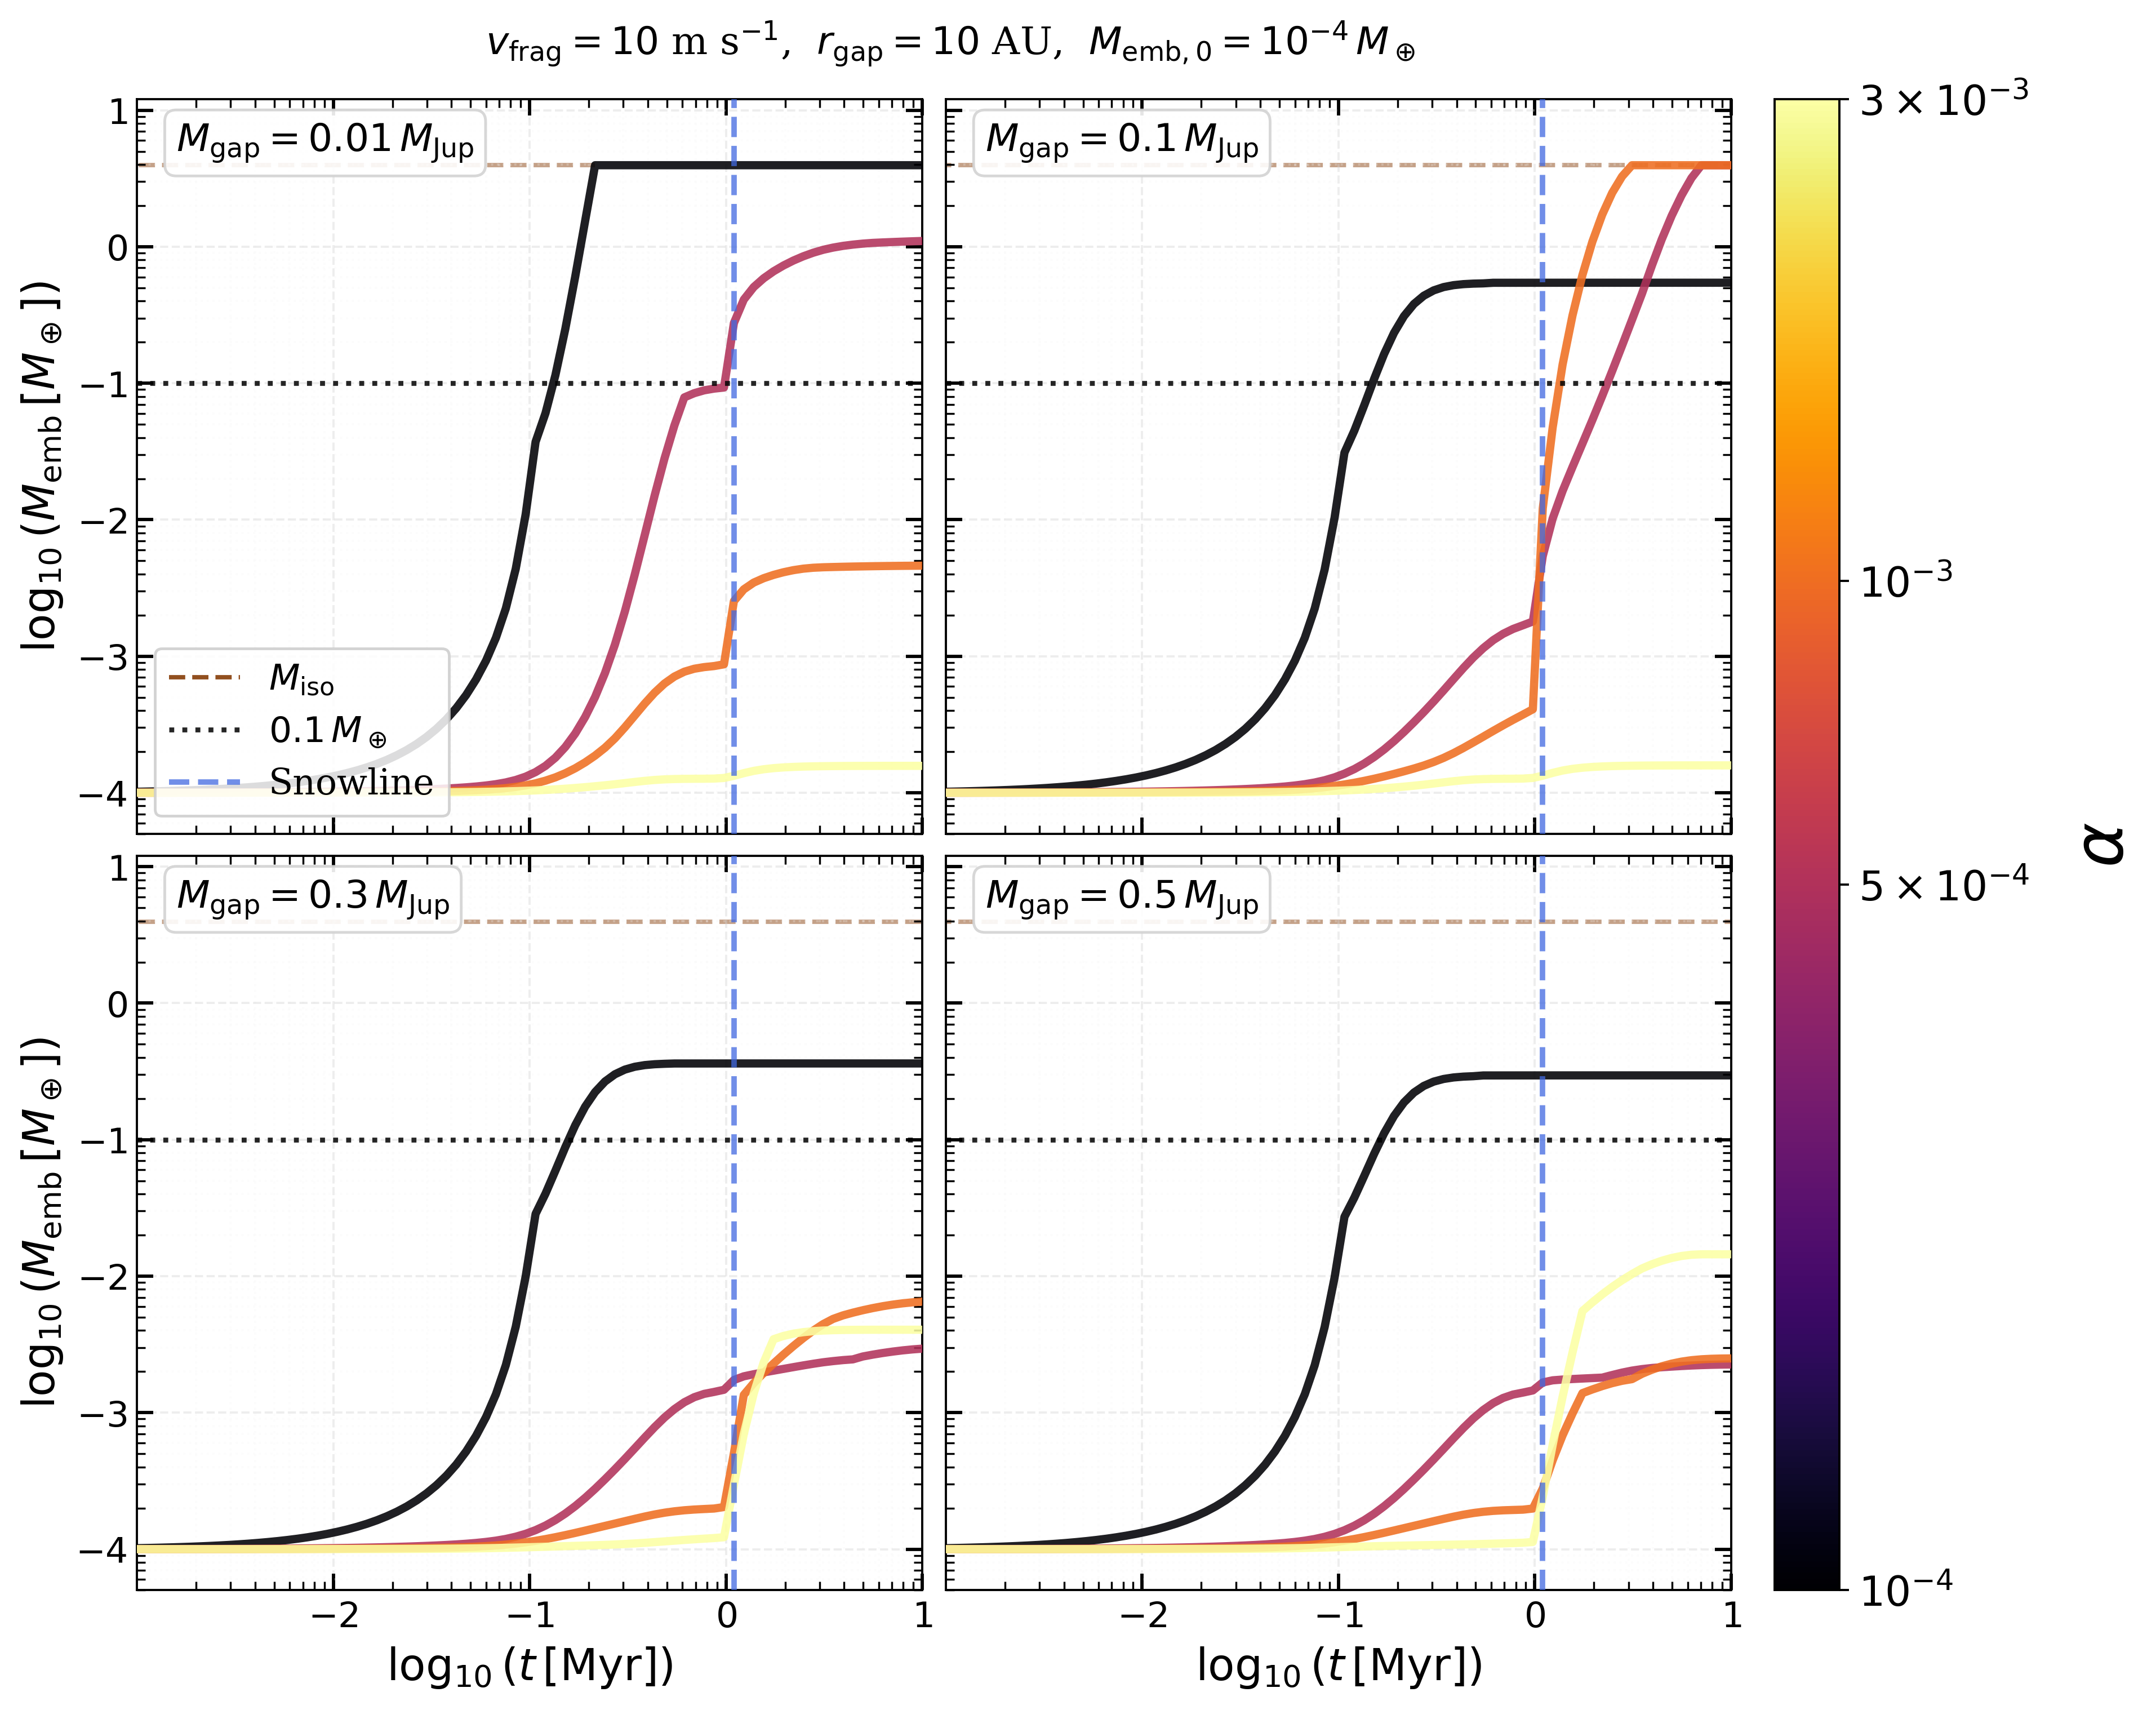
\includegraphics[width=0.8\textwidth]{figures/4_fig_resultados/figura_B_regimenes_mgap.png}
    \caption{
    Evolución temporal de la masa del embrión para distintos niveles de turbulencia. Cada panel corresponde a una masa diferente del planeta que abre el gap ($M_{\rm gap}=0.01$, $0.1$, $0.3$ y $0.5\,M_{\rm Jup}$). El color de las trayectorias representa el parámetro turbulento $\alpha$. Se mantiene fijo $v_{\rm frag}=10\,{\rm m\,s^{-1}}$, $r_{\rm gap}=10\,{\rm AU}$ y $M_{\rm emb,0}=10^{-4}\,M_\oplus$. Los ejes y las líneas de referencia son los mismos que en la Figura~\ref{fig:gap_sinusoidal}.
    }
    \label{fig:regimenes_alpha}
\end{figure}

En todas las configuraciones, las trayectorias correspondientes a los menores valores de $\alpha$ alcanzan las mayores masas finales, mientras que el crecimiento disminuye progresivamente al aumentar la turbulencia.

La dependencia con $\alpha$ varía entre paneles. En particular, el caso con $M_{\rm gap}=0.1\,M_{\rm Jup}$ presenta el mayor número de trayectorias que superan el umbral de $0.1\,M_\oplus$, mientras que para el resto de las masas del gap únicamente los valores más bajos de $\alpha$ alcanzan masas comparables.
% =========================================================
\section{Síntesis Poblacional: La Isla de Crecimiento}
\label{sec:sintesis_poblacional}
% =========================================================

Esta sección presenta un análisis global de la población final de embriones obtenida en las simulaciones, evaluando la masa final alcanzada y su composición final (fracción de agua) bajo diferentes regímenes de los parámetros explorados.

% =========================================================
\invisiblesubsection{Dinámica temporal del gap}
% =========================================================

La Figura~\ref{fig:delayed_gap} presenta la masa final del embrión en función de la fracción de agua para un escenario de alta turbulencia ($\alpha = 0.001$) con un gap ubicado en $10\,{\rm AU}$. En este panel, el tiempo en el que se forma la subestructura ($t_{\rm gap}$) se indica mediante la escala de color, mientras que la masa del planeta responsable del gap define la forma del marcador.

\begin{figure}[h!]
    \centering
    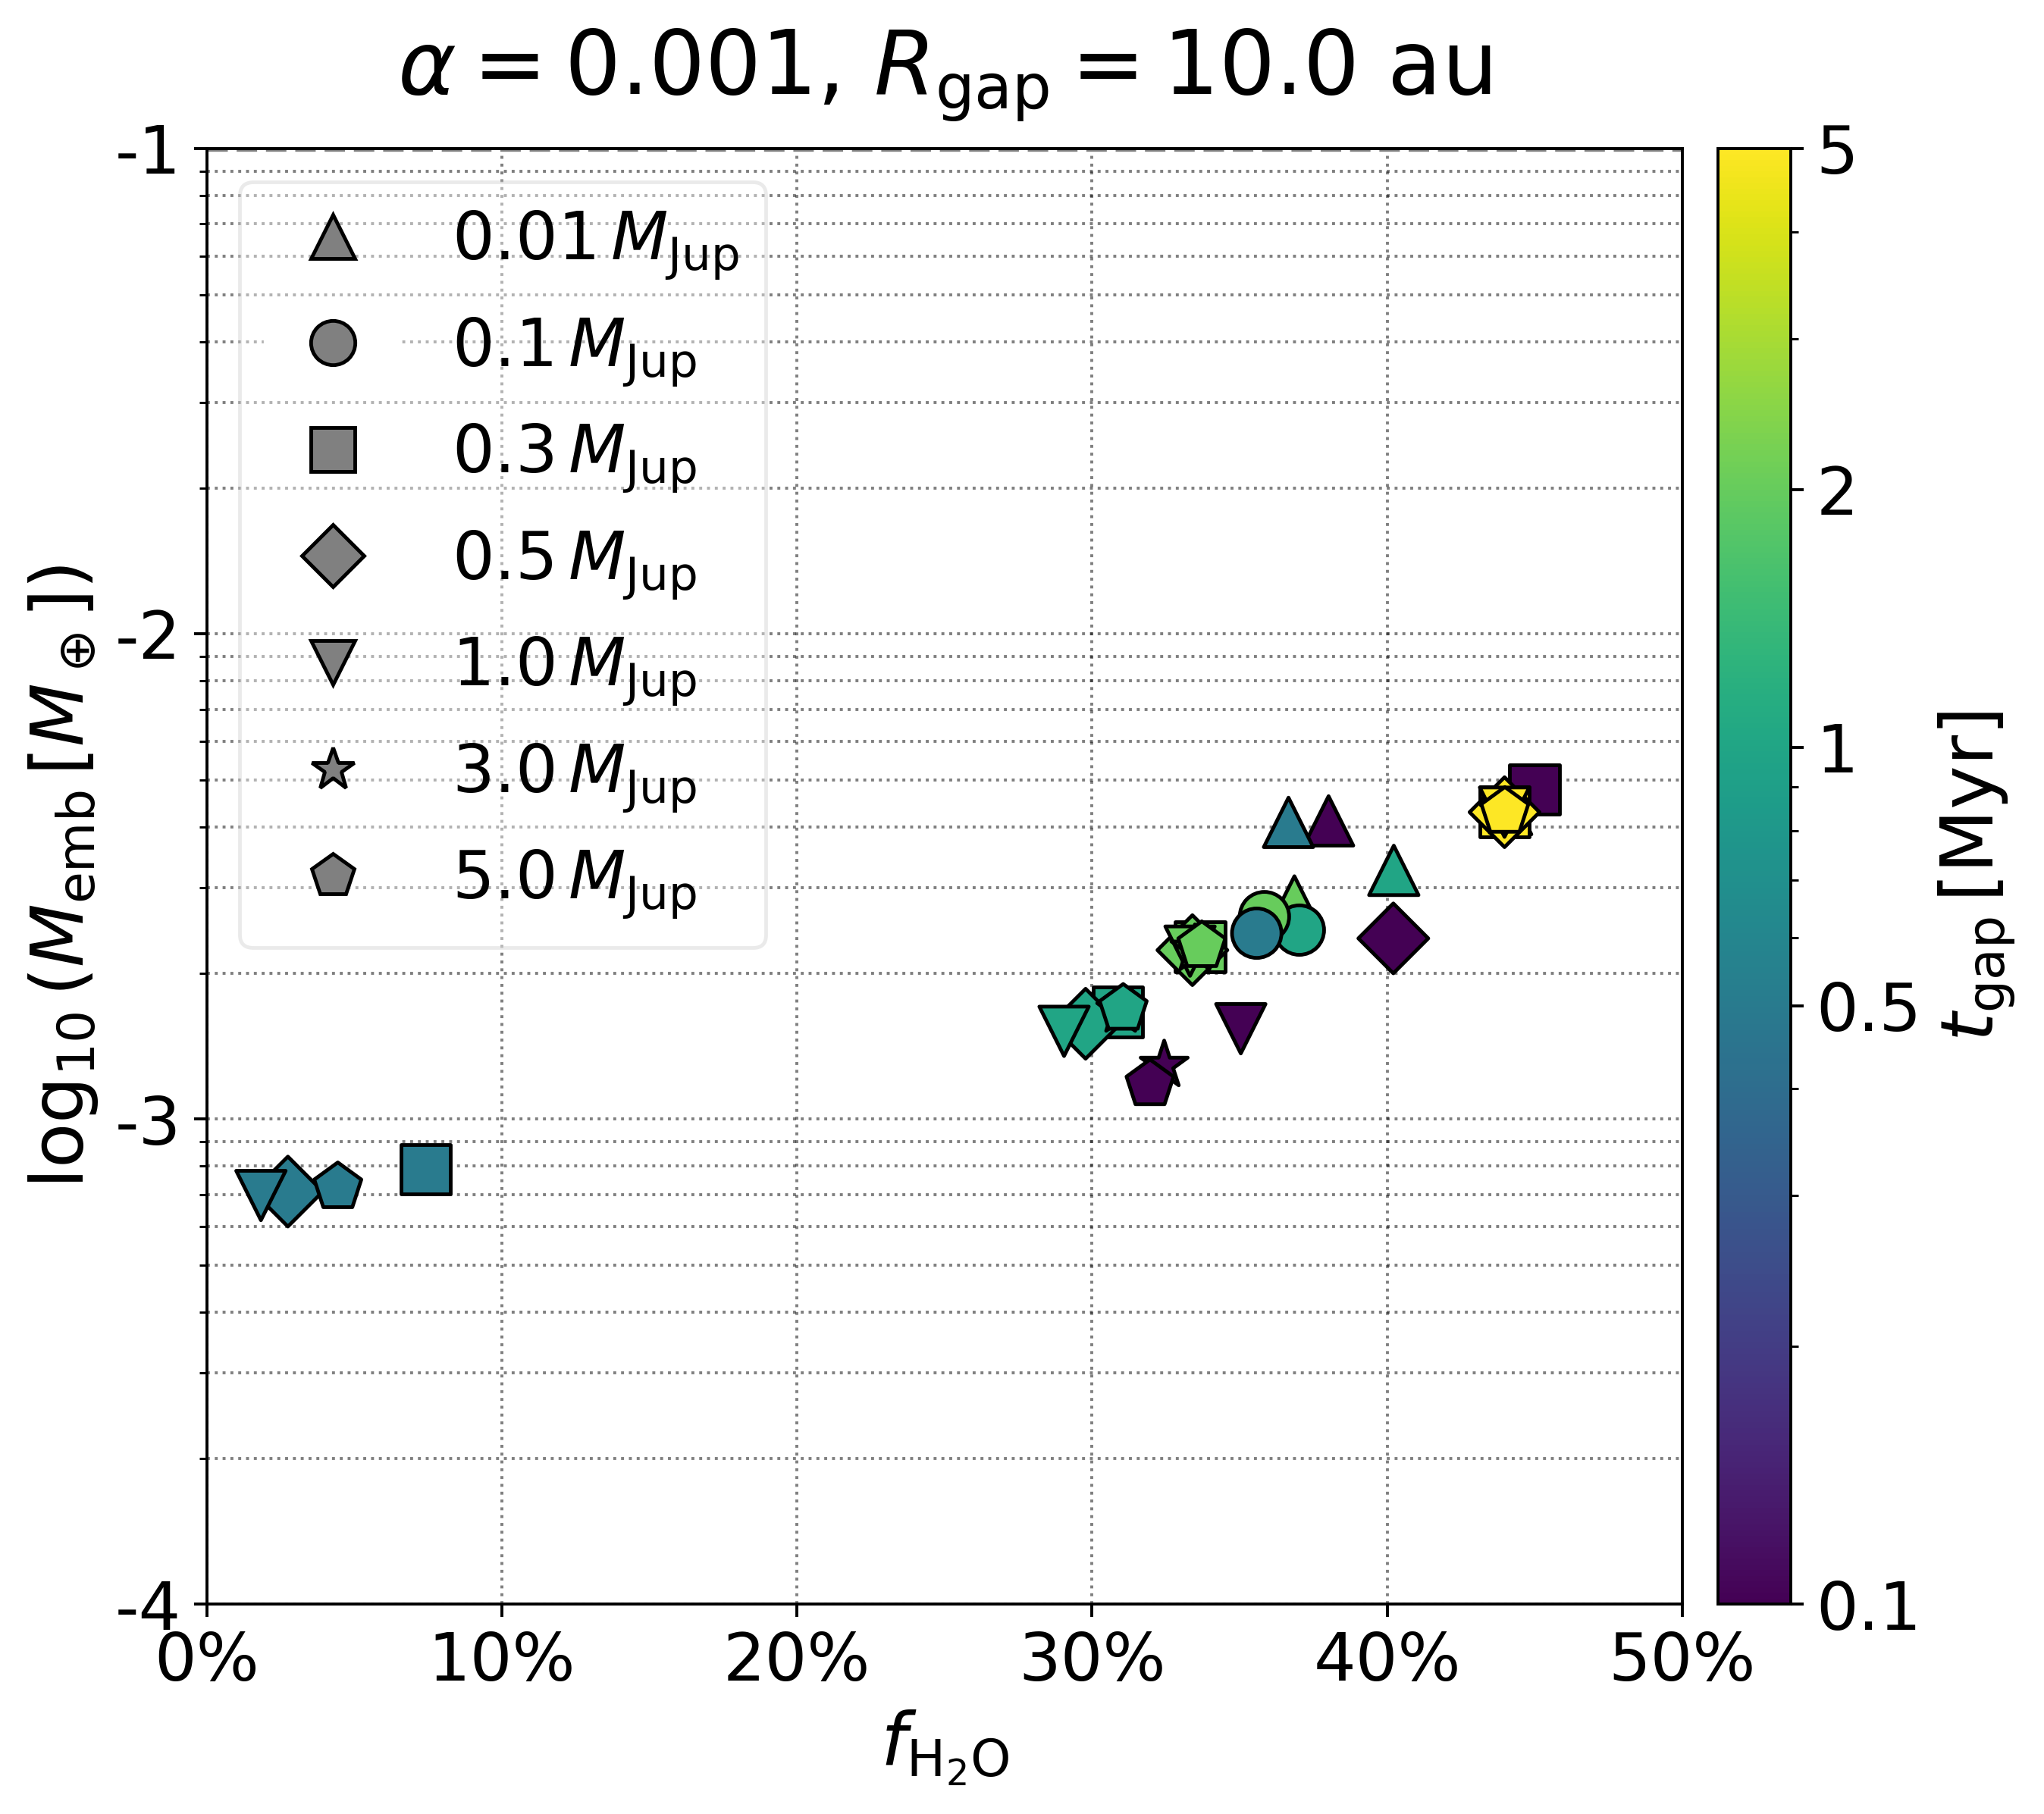
\includegraphics[width=0.75\textwidth]{figures/4.2_resultados/resultados_delayed_1x1_markers.png}
    \caption{Masa final del embrión (en escala logaritmica) versus fracción de agua (en porcentaje) para un disco con turbulencia $\alpha = 0.001$ y un gap en $r_{\rm gap}=10\,{\rm AU}$. El color de los marcadores representa el tiempo en el que se introduce el gap en la simulación ($t_{\rm gap}$) y la forma del marcador indica la masa del perturbador ($M_{\rm gap}$).}
    \label{fig:delayed_gap}
\end{figure}

Se observa una tendencia principal diagonal donde la mayoría de los casos se agrupan con fracciones de agua elevadas (entre $30\%$ y $50\%$). En este grupo convergen todas las masas de gap exploradas y una amplia variedad de tiempos de formación. Fuera de esta aglomeración, se distingue un único grupo de casos aislados en la zona de bajas fracciones de agua ($< 10\%$). Estos marcadores corresponden exclusivamente a simulaciones con un tiempo de formación de gap temprano (tonos oscuros/cian) y masas de perturbador mayores o iguales a $0.3\,M_{\rm Jup}$ (cuadrados, pentágonos, hexágonos y rombos).

% =========================================================
\invisiblesubsection{Mapa de parámetros globales}
% =========================================================

Para expandir el análisis a la grilla completa de simulaciones, la Figura~\ref{fig:mapa_global} resume los resultados variando la turbulencia, la velocidad de fragmentación y las características espaciales de la subestructura. 

\begin{figure}[h!]
    \centering
    
\includegraphics[width=\textwidth]{figures/4.2_resultados/resultados_bubble.png} 
    \caption{Mapa de resultados que sintetiza la población final. Las columnas varían la turbulencia $\alpha$ y las filas la velocidad de fragmentación $v_{\rm frag}$. El tamaño del círculo representa una aproximación de la masa final y el color indica la fracción de agua. Los marcadores circulares indican casos exitosos ($\ge 0.1\,M_\oplus$), mientras que los triángulos invertidos representan fracasos.}
    \label{fig:mapa_global}
\end{figure}

El panel muestra que el mayor número de casos exitosos (marcadores circulares) ocurre para bajas turbulencias ($\alpha=10^{-4}$) y altas velocidades de fragmentación ($v_{\rm frag}=10\,{\rm m\,s^{-1}}$). Particularmente para este último valor de $v_{\rm frag}$ (fila inferior), se aprecia una franja horizontal de éxito sostenido concentrada en profundidades de gap entre $0.05$ y $0.1\,M_{\rm Jup}$. Esta banda mantiene la formación de embriones masivos, con altas fracciones de agua (tonos naranjas/amarillos), incluso al aumentar la turbulencia hacia las columnas de la derecha. Las configuraciones con gaps más profundos o velocidades de fragmentación menores presentan predominantemente marcadores de fracaso.

% =========================================================
\invisiblesubsection{Distribución composicional}
% =========================================================

La Figura~\ref{fig:facet_lineal} examina explícitamente la relación entre la masa final y la composición para las distintas arquitecturas del disco (gap único y perfil sinusoidal). 

\begin{figure}[h!]
    \centering
    
\includegraphics[width=\textwidth]{figures/4.2_resultados/figura_C_facet_combinado_lineal.png}
    \caption{Masa final del embrión versus fracción de agua (escala lineal) para distintos valores de turbulencia (columnas). La fila superior corresponde a un gap único y la inferior a un perfil sinusoidal. El color indica la velocidad de fragmentación.}
    \label{fig:facet_lineal}
\end{figure}

Al observar la secuencia de izquierda a derecha (incremento de $\alpha$), la distribución de la población muestra un colapso generalizado hacia el extremo derecho de los paneles. Para $\alpha \ge 5\times10^{-4}$, la inmensa mayoría de los embriones que superan el umbral de masa exhiben fracciones de agua cercanas al $50\%$.

Sin embargo, en la primera columna correspondiente a la turbulencia más baja ($\alpha=10^{-4}$), la distribución es notablemente diferente. Además de los casos ricos en agua, se acumula un conjunto visible de simulaciones que alcanzan masas por encima de $0.1\,M_\oplus$ manteniendo fracciones de agua sumamente bajas (cercanas al margen izquierdo del panel).

Para visualizar con mayor precisión esta subpoblación específica, la Figura~\ref{fig:facet_log} presenta la misma distribución para $\alpha=10^{-4}$, restringiendo el eje horizontal al rango de $0\%$ a $10\%$ mediante una escala logarítmica.

\begin{figure}[h!]
    \centering
    
\includegraphics[width=0.85\textwidth]{figures/4.2_resultados/figura_C_facet_combinado_log_10pct.png}
    \caption{Detalle de la masa final versus fracción de agua en escala logarítmica para $\alpha=10^{-4}$, enfocado en el rango de $0\%$ a $10\%$ de composición de agua. El sombreado destaca distintas zonas de acumulación en los escenarios de gap único (arriba) y perfil sinusoidal (abajo).}
    \label{fig:facet_log}
\end{figure}

El gráfico evidencia claramente la existencia de una agrupación de planetas masivos y predominantemente secos, los cuales exhiben fracciones de agua de entre $0\%$ y $2\%$. Esta subpoblación se distingue nítidamente tanto en la configuración de gap único como en la sinusoidal bajo este nivel específico de turbulencia.
% =========================================================
% CAPÍTULO 5 — DISCUSIÓN
% =========================================================

\chapter{Discusión}
\label{cap:discusion}
%=========================================================
\section{Regulación del Flujo de Pebbles y el Filtro Aerodinámico}
%=========================================================

El resultado central de este trabajo es que las subestructuras no actúan únicamente como trampas estáticas de polvo, sino como reguladores temporales del flujo radial de \textit{pebbles}. En lugar de modificar exclusivamente la cantidad total de sólidos disponibles para la acreción, alteran la cronología y la duración del suministro de material hacia los embriones planetarios. Como consecuencia, la evolución temporal del flujo de \textit{pebbles} emerge como el mecanismo que conecta el crecimiento planetario con la composición final de los planetas.

La dinámica de este proceso es evidente en los diagramas de Hovmöller (Figuras \ref{fig:hovmoller_vfrag}--\ref{fig:hovmoller_turbulencia}), donde se observa un incremento pronunciado en la tasa de acreción alrededor de $1\,{\rm Myr}$. Este evento coincide con el paso de la \textit{snowline} por la órbita del embrión. Cuando esto ocurre, la disminución de la velocidad de fragmentación ($v_{\rm frag}$, desde $10\,{\rm m\,s^{-1}}$ para agregados ricos en hielo hasta $1\,{\rm m\,s^{-1}}$ para silicatos) reduce el tamaño máximo alcanzable por los \textit{pebbles} y, en consecuencia, su número de Stokes. La población sólida previamente retenida en la trampa de presión experimenta entonces un episodio de liberación hacia el disco interno, incrementando temporalmente el flujo de \textit{pebbles} disponible para la acreción.

Este comportamiento constituye una manifestación natural del escenario de \textit{pebble snow} propuesto por \citet{Drazkowska2021}. En dicho escenario, la migración de la \textit{snowline} controla el transporte de material rico en hielo hacia regiones inicialmente secas del disco. Nuestros resultados muestran que la presencia de subestructuras potencia este mecanismo al generar reservorios temporales de \textit{pebbles}, cuya liberación ocurre precisamente cuando la evolución térmica modifica las propiedades de fragmentación del polvo. De este modo, el enriquecimiento tardío en agua no depende únicamente de la migración de la \textit{snowline}, sino también de la capacidad de las trampas de presión para almacenar y liberar sólidos a lo largo de la evolución del disco.

La importancia de esta regulación temporal resulta consistente con estudios recientes sobre la evolución del polvo en discos estructurados. Por ejemplo, \citet{Appelgren2025} muestran que las subestructuras modifican significativamente la evolución del flujo de \textit{pebbles} mediante la retención de sólidos, mientras que \citet{Lau2024} encuentran que la presencia de anillos de presión altera de manera sustancial el suministro de material hacia las regiones internas respecto a los modelos de discos suaves. En este contexto, nuestros resultados extienden estas ideas al mostrar cómo dicha modulación temporal del flujo se traduce directamente en diferencias tanto en el crecimiento planetario como en el contenido final de agua.

La relevancia del mecanismo propuesto se hace aún más evidente al analizar el caso de control donde se elimina el contraste en la velocidad de fragmentación, adoptando un valor uniforme de $v_{\rm frag}=1\,{\rm m\,s^{-1}}$ en todo el disco. En estas simulaciones, el tamaño máximo de los \textit{pebbles} y su número de Stokes evolucionan de forma continua, desapareciendo el episodio de liberación asociado al paso de la \textit{snowline}. Como consecuencia, la trampa de presión actúa únicamente como un filtro aerodinámico estático, reduciendo de manera sostenida el flujo de sólidos hacia el embrión. Bajo estas condiciones, el crecimiento permanece limitado y las masas finales no superan el régimen marciano.

En conjunto, estos resultados indican que el crecimiento planetario más eficiente no ocurre cuando las trampas bloquean completamente el transporte de sólidos, sino cuando actúan como reservorios temporales capaces de almacenar y liberar \textit{pebbles} conforme evoluciona la estructura térmica del disco. En este sentido, las subestructuras funcionan como reguladores dinámicos del flujo de \textit{pebbles}, más que como simples barreras aerodinámicas.

%=========================================================
%=========================================================
\section{La Isla de Crecimiento y la Influencia de la Turbulencia}
%=========================================================

La síntesis poblacional revela que el crecimiento planetario eficiente no varía de manera monótona con los parámetros del disco, sino que se concentra en una región bien definida del espacio de parámetros, la cual hemos denominado \textit{Isla de Crecimiento} (Figura \ref{fig:mapa_global}). En nuestras simulaciones, esta región se caracteriza por viscosidades moderadas o bajas ($\alpha \lesssim 10^{-3}$) y masas de los gaps del orden de $M_{\rm gap}\sim0.1\,M_{\rm Jup}$. Dentro de este régimen, los embriones alcanzan masas superiores a $0.1\,M_\oplus$, mientras que fuera de él el crecimiento se vuelve significativamente menos eficiente.

La existencia de esta región óptima refleja el equilibrio entre dos procesos contrapuestos. Por una parte, subestructuras demasiado débiles permiten que los \textit{pebbles} deriven rápidamente hacia la estrella antes de ser incorporados por el embrión. Por otra, gaps demasiado masivos ($M_{\rm gap}\gtrsim0.3\,M_{\rm Jup}$) retienen el material sólido con tal eficiencia que reducen drásticamente el flujo disponible para la acreción. El crecimiento planetario más eficiente ocurre, por tanto, cuando las trampas de presión funcionan como reservorios temporales capaces de regular el suministro de sólidos sin bloquearlo completamente.

Los diagramas de masa poblacional muestran además que esta ventana de formación depende de manera crítica del nivel de turbulencia. Para $\alpha\ge3\times10^{-3}$ ninguna configuración alcanza $0.1\,M_\oplus$. 
En el extremo opuesto, cuando $\alpha \sim 10^{-4}$ acoplado a $v_{\rm frag} = 10$ m/s, 
la acumulación es tan eficiente que emerge una bimodalidad composicional 
que se discute en la Sección 5.3. Físicamente, un incremento de la turbulencia aumenta las velocidades relativas entre partículas, limita su crecimiento por fragmentación y reduce sus números de Stokes. Como consecuencia, los \textit{pebbles} permanecen más fuertemente acoplados al gas, incrementando la escala de altura del polvo ($H_{\rm d}$) y desplazando la acreción hacia un régimen tridimensional menos eficiente.

Este comportamiento resulta consistente con el marco teórico de la acreción de \textit{pebbles}, donde la eficiencia de captura depende fuertemente tanto del número de Stokes como del espesor de la capa de polvo \citep{Bitsch2015,Ataiee2018}. Asimismo, nuestros resultados son compatibles con escenarios en los que regiones de baja turbulencia (\textit{dead zones}) favorecen el crecimiento planetario al permitir una mayor sedimentación del polvo y una transición hacia un régimen de acreción predominantemente bidimensional. En este contexto, la \textit{Isla de Crecimiento} puede interpretarse como la manifestación poblacional del equilibrio entre la regulación temporal del flujo de \textit{pebbles} por las subestructuras y la eficiencia de la acreción controlada por la turbulencia del disco.


%=========================================================
\section{Bifurcación Poblacional: Planetas Secos y Ricos en Agua}
%=========================================================

Las Figuras \ref{fig:facet_lineal} y \ref{fig:facet_log} muestran una tendencia general entre la masa final de los embriones y su contenido de agua. En la mayor parte del espacio de parámetros explorado, los planetas más masivos alcanzan también las mayores fracciones de agua, del orden del $50\%$. Esta correlación no implica una relación causal directa entre la masa planetaria y el contenido de agua; en cambio, ambas propiedades emergen como consecuencia de un mismo mecanismo físico: la regulación temporal del flujo de \textit{pebbles} por las subestructuras del disco.

En los regímenes donde las trampas de presión almacenan eficientemente material exterior, el crecimiento del embrión se prolonga durante tiempos comparables con la migración de la \textit{snowline}. Como resultado, una fracción significativa de la masa incorporada en las etapas finales proviene del reservorio de \textit{pebbles} ricos en hielo liberado tras el paso de la \textit{snowline}. Este enriquecimiento tardío constituye una manifestación del escenario de \textit{pebble snow}, donde la evolución térmica del disco y el transporte radial de sólidos actúan conjuntamente para suministrar agua a las regiones internas \citep{Drazkowska2021}.

Sin embargo, el análisis en escala logarítmica (Figura \ref{fig:facet_log}) revela una excepción particularmente interesante. Para el régimen de muy baja turbulencia ($\alpha = 10^{-4}$) combinado con una alta velocidad de fragmentación ($v_{\rm frag}=10\,{\rm m\,s^{-1}}$), emerge una población de embriones masivos ($\ge0.1\,M_\oplus$) con fracciones de agua inferiores al $2\%$. En este caso, la elevada eficiencia de la acreción permite que el embrión alcance rápidamente su masa de aislamiento utilizando casi exclusivamente el reservorio local de silicatos. Cuando posteriormente la \textit{snowline} migra hacia el interior y libera el reservorio rico en hielos, el planeta ha reducido drásticamente su capacidad de seguir incorporando material, preservando así una composición predominantemente rocosa.

Este comportamiento pone de manifiesto que la cronología relativa entre el crecimiento planetario y la evolución de la \textit{snowline} constituye un factor determinante para la composición final de los planetas. Dependiendo de cuál de estos procesos domine primero, un mismo disco puede producir tanto planetas ricos en agua como planetas predominantemente rocosos.

Es importante señalar que las masas extremas obtenidas para $\alpha = 10^{-4}$ deben interpretarse con cautela. En la implementación actual, PA3Py se ejecuta en post-procesado y no retroalimenta la evolución de TriPoDPy mediante la remoción de la masa ya acretada. En condiciones de muy alta densidad superficial de sólidos, esta aproximación puede conducir a una sobreestimación cuantitativa de las masas finales. No obstante, esta limitación afecta principalmente los valores absolutos de masa y no modifica la tendencia cualitativa observada: la regulación temporal del flujo de \textit{pebbles} puede conducir a dos trayectorias evolutivas claramente diferenciadas, una dominada por el enriquecimiento tardío en agua y otra por un crecimiento temprano predominantemente rocoso.


%=========================================================
\section{Comparación con Modelos Clásicos de Discos Suaves}
%=========================================================

En los modelos de discos suaves, la deriva radial conduce a un decaimiento casi monótono del flujo de sólidos hacia las regiones internas \citep{Lambrechts2014,Ormel2017}. Bajo este paradigma clásico, la composición final de los planetas dependía casi exclusivamente de su posición orbital inicial respecto a la línea de nieve, limitando la diversidad química observada en la síntesis poblacional.

Las subestructuras rompen este comportamiento al introducir episodios discretos de acumulación y liberación de sólidos. Esta modulación temporal trasciende el concepto de barrera aerodinámica estática, proporcionando un marco físico donde el transporte de volátiles se desacopla parcialmente del decaimiento global del disco. Al retener material primigenio exterior y liberarlo de manera tardía, los discos estructurados ofrecen un camino natural para explicar el transporte de agua hacia las regiones terrestres.

En este contexto, la cronología del suministro de sólidos resulta ser un factor tan determinante como el inventario inicial de masa. La interacción entre la migración de la isoterma de sublimación y la permeabilidad variable de las trampas de presión permite generar un espectro composicional mucho más amplio que el obtenido tradicionalmente en perfiles de disco suaves, conciliando la física de acreción con la diversidad observada en sistemas planetarios complejos.



%=========================================================
\section{Limitaciones del Modelo}
%=========================================================

Como todo modelo de formación planetaria, el marco desarrollado en este trabajo incorpora diversas simplificaciones que deben considerarse al interpretar los resultados. No obstante, estas limitaciones afectan principalmente la cuantificación precisa de las masas y composiciones finales, sin modificar las tendencias físicas identificadas a lo largo de las simulaciones.

En primer lugar, la evolución térmica del disco se representa mediante una parametrización basada en los modelos de \citet{Oka2011}. En consecuencia, la posición de la \textit{snowline} no se obtiene de manera auto-consistente a partir de la evolución dinámica del disco, sino que corresponde a una aproximación de su migración temporal. Si bien esta simplificación puede modificar el instante exacto en que la \textit{snowline} atraviesa la órbita del embrión, no altera el mecanismo físico identificado en este trabajo, donde la cronología relativa entre la migración de la \textit{snowline} y la liberación del reservorio de pebbles controla el enriquecimiento en agua.

Asimismo, el modelo considera una descripción unidimensional del disco protoplanetario. Procesos tridimensionales como la sedimentación vertical del polvo, la estructura vertical de los gaps o posibles inestabilidades hidrodinámicas no son resueltos explícitamente y se encuentran incorporados mediante parametrizaciones. Aunque estos efectos pueden modificar cuantitativamente la eficiencia de las trampas de presión, no se espera que alteren el comportamiento cualitativo asociado al almacenamiento y posterior liberación de pebbles.

Una limitación adicional corresponde al acoplamiento entre TriPoDPy y PA3Py. En la implementación actual, la acreción planetaria se calcula como un proceso de post-procesado, por lo que la masa incorporada por el embrión no retroalimenta la evolución del disco. En consecuencia, la densidad superficial de pebbles no disminuye localmente debido a la acreción, lo que podría conducir a una sobreestimación moderada de las masas finales y de la cantidad total de agua incorporada. Sin embargo, dado que el crecimiento se encuentra limitado por la masa de aislamiento, este efecto permanece acotado en la mayoría de las simulaciones exitosas.

Finalmente, el modelo adopta una descripción simplificada de la composición química del polvo, distinguiendo únicamente entre material seco y material rico en agua. Otros volátiles importantes, como CO, CO$_2$ o NH$_3$, no son considerados explícitamente. En consecuencia, las fracciones de agua obtenidas deben interpretarse como una aproximación al contenido total de volátiles y no como una descripción química completa de los planetas formados.

En conjunto, estas simplificaciones no modifican la principal conclusión de este trabajo: las subestructuras del disco alteran la evolución temporal del flujo de pebbles y, como consecuencia, regulan simultáneamente el crecimiento planetario y el transporte de agua hacia las regiones internas.

%=========================================================


% =========================================================
% CONCLUSIONES
% =========================================================

\chapter{Conclusiones}
\label{cap:conclusiones}

%=========================================================
\section{Síntesis de Resultados y Aportes Principales}
%=========================================================

Este trabajo abordó la pregunta central planteada en la Sección 1.6: ¿cómo modifican las subestructuras de un disco protoplanetario el crecimiento y la composición de planetas terrestres mediante acreción de \textit{pebbles}? Los resultados obtenidos muestran que las subestructuras no sólo alteran la cantidad de sólidos disponibles para la acreción, sino también el momento en que éstos alcanzan al embrión. Como consecuencia, la evolución temporal del flujo de \textit{pebbles} emerge como el mecanismo físico que controla simultáneamente el crecimiento planetario y el contenido final de agua.

El análisis de 5006 trayectorias evolutivas permitió identificar tendencias robustas en función de la turbulencia del disco, la profundidad de las trampas de presión y las propiedades de fragmentación del polvo. En conjunto, los resultados muestran que la interacción entre la evolución térmica del disco y las subestructuras genera una amplia diversidad de trayectorias evolutivas, estableciendo una conexión directa entre la dinámica del disco protoplanetario y las propiedades finales de los planetas formados.

Los principales aportes de este trabajo pueden resumirse en los siguientes puntos:

\begin{enumerate}
    \item Se desarrolló un marco de trabajo que acopla la evolución del polvo calculada con TriPoDPy y la acreción planetaria mediante PA3Py, permitiendo estudiar de forma eficiente la formación de planetas terrestres en discos con subestructuras.

    \item Se implementó una evolución temporal parametrizada de la \textit{snowline}, basada en el decaimiento de la tasa de acreción estelar y en modelos analíticos de estructura térmica del disco, incorporando el transporte temporal de volátiles durante la formación planetaria.

    \item Se identificó una \textit{Isla de Crecimiento}, delimitando el régimen de parámetros donde la formación planetaria resulta más eficiente, caracterizado por turbulencias moderadas o bajas ($\alpha \lesssim 10^{-3}$) y trampas de presión de profundidad intermedia ($M_{\rm gap}\sim0.05-0.1\,M_{\rm Jup}$).

    \item Se mostró que la regulación temporal del flujo de \textit{pebbles} constituye el mecanismo físico que vincula el crecimiento planetario con la composición final de los planetas, generando una correlación entre masa y contenido de agua que surge de una cronología común y no de una relación causal directa entre ambas propiedades.

    \item Se encontró que, dentro de las arquitecturas exploradas, la profundidad de las trampas de presión ejerce un control significativamente mayor sobre el crecimiento y la composición planetaria que el número de subestructuras presentes en el disco, indicando que la eficiencia del atrapamiento resulta más importante que la complejidad de la arquitectura.

    \item Se identificó una población de planetas masivos pero pobres en agua bajo condiciones de muy baja turbulencia, evidenciando que pequeñas diferencias en la cronología del suministro de \textit{pebbles} pueden conducir a composiciones planetarias radicalmente distintas.
\end{enumerate}

%=========================================================
\section{La Regulación Temporal del Flujo de Pebbles y la Isla de Crecimiento}
%=========================================================

El principal resultado físico de este trabajo es que el crecimiento planetario eficiente depende más de la distribución temporal del suministro de sólidos que de la cantidad total de material disponible. Las subestructuras transforman un flujo radial originalmente continuo en un suministro episódico, caracterizado por etapas de almacenamiento y liberación de \textit{pebbles} conforme evoluciona el disco.

La denominada \textit{Isla de Crecimiento} constituye la manifestación cuantitativa de este mecanismo. Nuestros resultados muestran que existe un equilibrio óptimo entre retención y suministro de sólidos. Trampas demasiado débiles permiten que los \textit{pebbles} deriven rápidamente hacia la estrella, mientras que trampas excesivamente profundas reducen de forma significativa el flujo disponible para la acreción. Sólo un régimen intermedio permite mantener un suministro prolongado capaz de sostener el crecimiento de los embriones hasta masas significativas.

La turbulencia desempeña un papel igualmente fundamental. Para valores elevados de $\alpha$, la difusión turbulenta incrementa la escala de altura del polvo y reduce la eficiencia de la acreción de \textit{pebbles}, mientras que en discos de baja turbulencia la sedimentación favorece una acreción más eficiente. En este contexto, la \textit{Isla de Crecimiento} representa el equilibrio entre el transporte radial de sólidos, la eficiencia del atrapamiento y la capacidad de los embriones para incorporarlos.

Un resultado adicional es que, para las arquitecturas consideradas en este trabajo, la profundidad de las trampas de presión controla mucho más fuertemente el crecimiento planetario y el enriquecimiento en agua que el número de subestructuras presentes en el disco. Tanto los modelos con un único \textit{gap} como aquellos con múltiples anillos presentan distribuciones composicionales similares cuando comparten profundidades equivalentes, lo que indica que la capacidad de almacenar y liberar \textit{pebbles} constituye el parámetro dominante.

%=========================================================
\section{Cronología del Flujo de Pebbles y Enriquecimiento en Agua}
%=========================================================

Los resultados obtenidos muestran que el enriquecimiento en agua de los planetas interiores no depende únicamente de la migración de la \textit{snowline}, sino de la interacción entre ésta y las subestructuras del disco. Las trampas de presión almacenan temporalmente \textit{pebbles} ricos en hielo, los cuales son liberados cuando la evolución térmica modifica las propiedades de fragmentación del polvo. En este sentido, las subestructuras no reemplazan el mecanismo de \textit{pebble snow}, sino que modifican su eficiencia y el momento en que el material rico en volátiles alcanza las regiones internas del disco.

La correlación observada entre la masa final de los planetas y su contenido de agua surge naturalmente de esta cronología. Los embriones cuyo crecimiento se prolonga hasta el episodio de liberación incorporan una fracción importante de material rico en hielo, mientras que aquellos que alcanzan tempranamente su masa de aislamiento conservan composiciones predominantemente rocosas. La población de planetas masivos pero secos identificada para $\alpha=10^{-4}$ constituye una evidencia indirecta de este mecanismo y demuestra que pequeñas variaciones en la cronología del crecimiento pueden generar trayectorias evolutivas y composiciones finales muy diferentes.

En consecuencia, la composición planetaria no queda determinada únicamente por el inventario inicial de sólidos del disco, sino también por el momento en que éstos se encuentran disponibles para la acreción. Esta interacción entre evolución térmica, transporte radial y subestructuras proporciona un mecanismo físico capaz de explicar la diversidad composicional observada en sistemas planetarios.


%========================================================= 
\section{Implicancias para la Formación Planetaria} 
%=========================================================

Los resultados obtenidos sugieren que los discos protoplanetarios con subestructuras de profundidad intermedia ($M_{\rm gap}\sim0.05-0.1\,M_{\rm Jup}$) y bajos niveles de turbulencia ($\alpha\lesssim10^{-3}$) constituyen los entornos más favorables para la formación de planetas terrestres mediante acreción de \textit{pebbles}. Bajo estas condiciones, las trampas de presión regulan eficientemente el transporte radial de sólidos, permitiendo mantener un suministro prolongado que favorece tanto el crecimiento del embrión como su enriquecimiento en volátiles. Este resultado proporciona una predicción física que puede contrastarse con observaciones de discos protoplanetarios. Las propiedades observables de las subestructuras, como la profundidad de los \textit{gaps} o la concentración de polvo en los anillos, pueden utilizarse como indicadores indirectos de la eficiencia del transporte de sólidos y, por consiguiente, del potencial de formación planetaria del sistema. En este contexto, nuestros resultados sugieren que la eficiencia de una trampa de presión depende principalmente de su capacidad para modular el flujo de \textit{pebbles}, más que del número de subestructuras presentes en el disco. En conjunto, este trabajo refuerza la idea de que la evolución temporal del disco desempeña un papel tan importante como su estructura espacial. La formación planetaria no depende únicamente de la existencia de reservorios de sólidos, sino también de la forma en que éstos son transportados y liberados durante la evolución del disco protoplanetario.

\section{Trabajo Futuro}
%=========================================================

Los resultados obtenidos en este trabajo abren diversas líneas de investigación orientadas a profundizar la relación entre la evolución del polvo y la formación planetaria.

Una extensión natural consiste en implementar un acoplamiento dinámico entre TriPoDPy y PA3Py, permitiendo que la acreción planetaria modifique de manera auto-consistente la distribución superficial de pebbles. Este desarrollo permitirá estudiar la competencia por material sólido entre múltiples embriones y evaluar con mayor precisión la evolución conjunta del disco y los planetas en formación.

Asimismo, resultará de interés incorporar una evolución térmica auto-consistente del disco, de modo que la posición de la \textit{snowline} responda directamente a la evolución de la estructura gaseosa y no a una parametrización externa. Esto permitirá estudiar con mayor detalle la sincronización entre la migración de la \textit{snowline}, la liberación de los reservorios de pebbles y el crecimiento planetario.

Otra extensión relevante consiste en incluir un tratamiento químico más completo, considerando múltiples especies volátiles y sus respectivas líneas de condensación. Esto permitirá investigar no sólo la fracción de agua, sino también la evolución de relaciones elementales como C/O, ampliamente utilizadas para interpretar observaciones de atmósferas exoplanetarias.

Finalmente, la incorporación de migración planetaria y la exploración de sistemas con múltiples embriones permitirán evaluar cómo la regulación temporal del flujo de pebbles interactúa con la evolución orbital de los planetas. Estos desarrollos contribuirán a construir un marco más completo para comprender de qué manera las subestructuras observadas en discos protoplanetarios condicionan tanto el crecimiento como la composición de los sistemas planetarios.



% --- APÉNDICES ---
\appendix
% % =========================================================
% APÉNDICE A — Sensibilidad Paramétrica y Controles de Robustez
% =========================================================

\chapter{Sensibilidad Paramétrica y Controles de Robustez}
\label{ap:sensibilidad}

Este apéndice complementa los resultados del Capítulo~\ref{cap:resultados} con
figuras adicionales que validan la robustez del mecanismo de \emph{Pebble Snow}
frente a variaciones en los parámetros de control. Las figuras aquí presentadas
no forman parte de la narrativa central, pero constituyen la evidencia empírica
que respalda las conclusiones del texto principal.

% ---------------------------------------------------------
\section{Impacto de $v_{\rm frag}$ sobre la Retención Aerodinámica}
% ---------------------------------------------------------

Las Figuras~\ref{fig:ap_hovmoller_v1} y~\ref{fig:ap_hovmoller_v3} presentan los
diagramas de Hovmöller equivalentes a la Figura~\ref{fig:hovmoller} pero para los
casos de control con $v_{\rm frag} = 1\text{ m/s}$ y $v_{\rm frag} = 3\text{ m/s}$
respectivamente.

\begin{figure}[htpb]
    \centering
    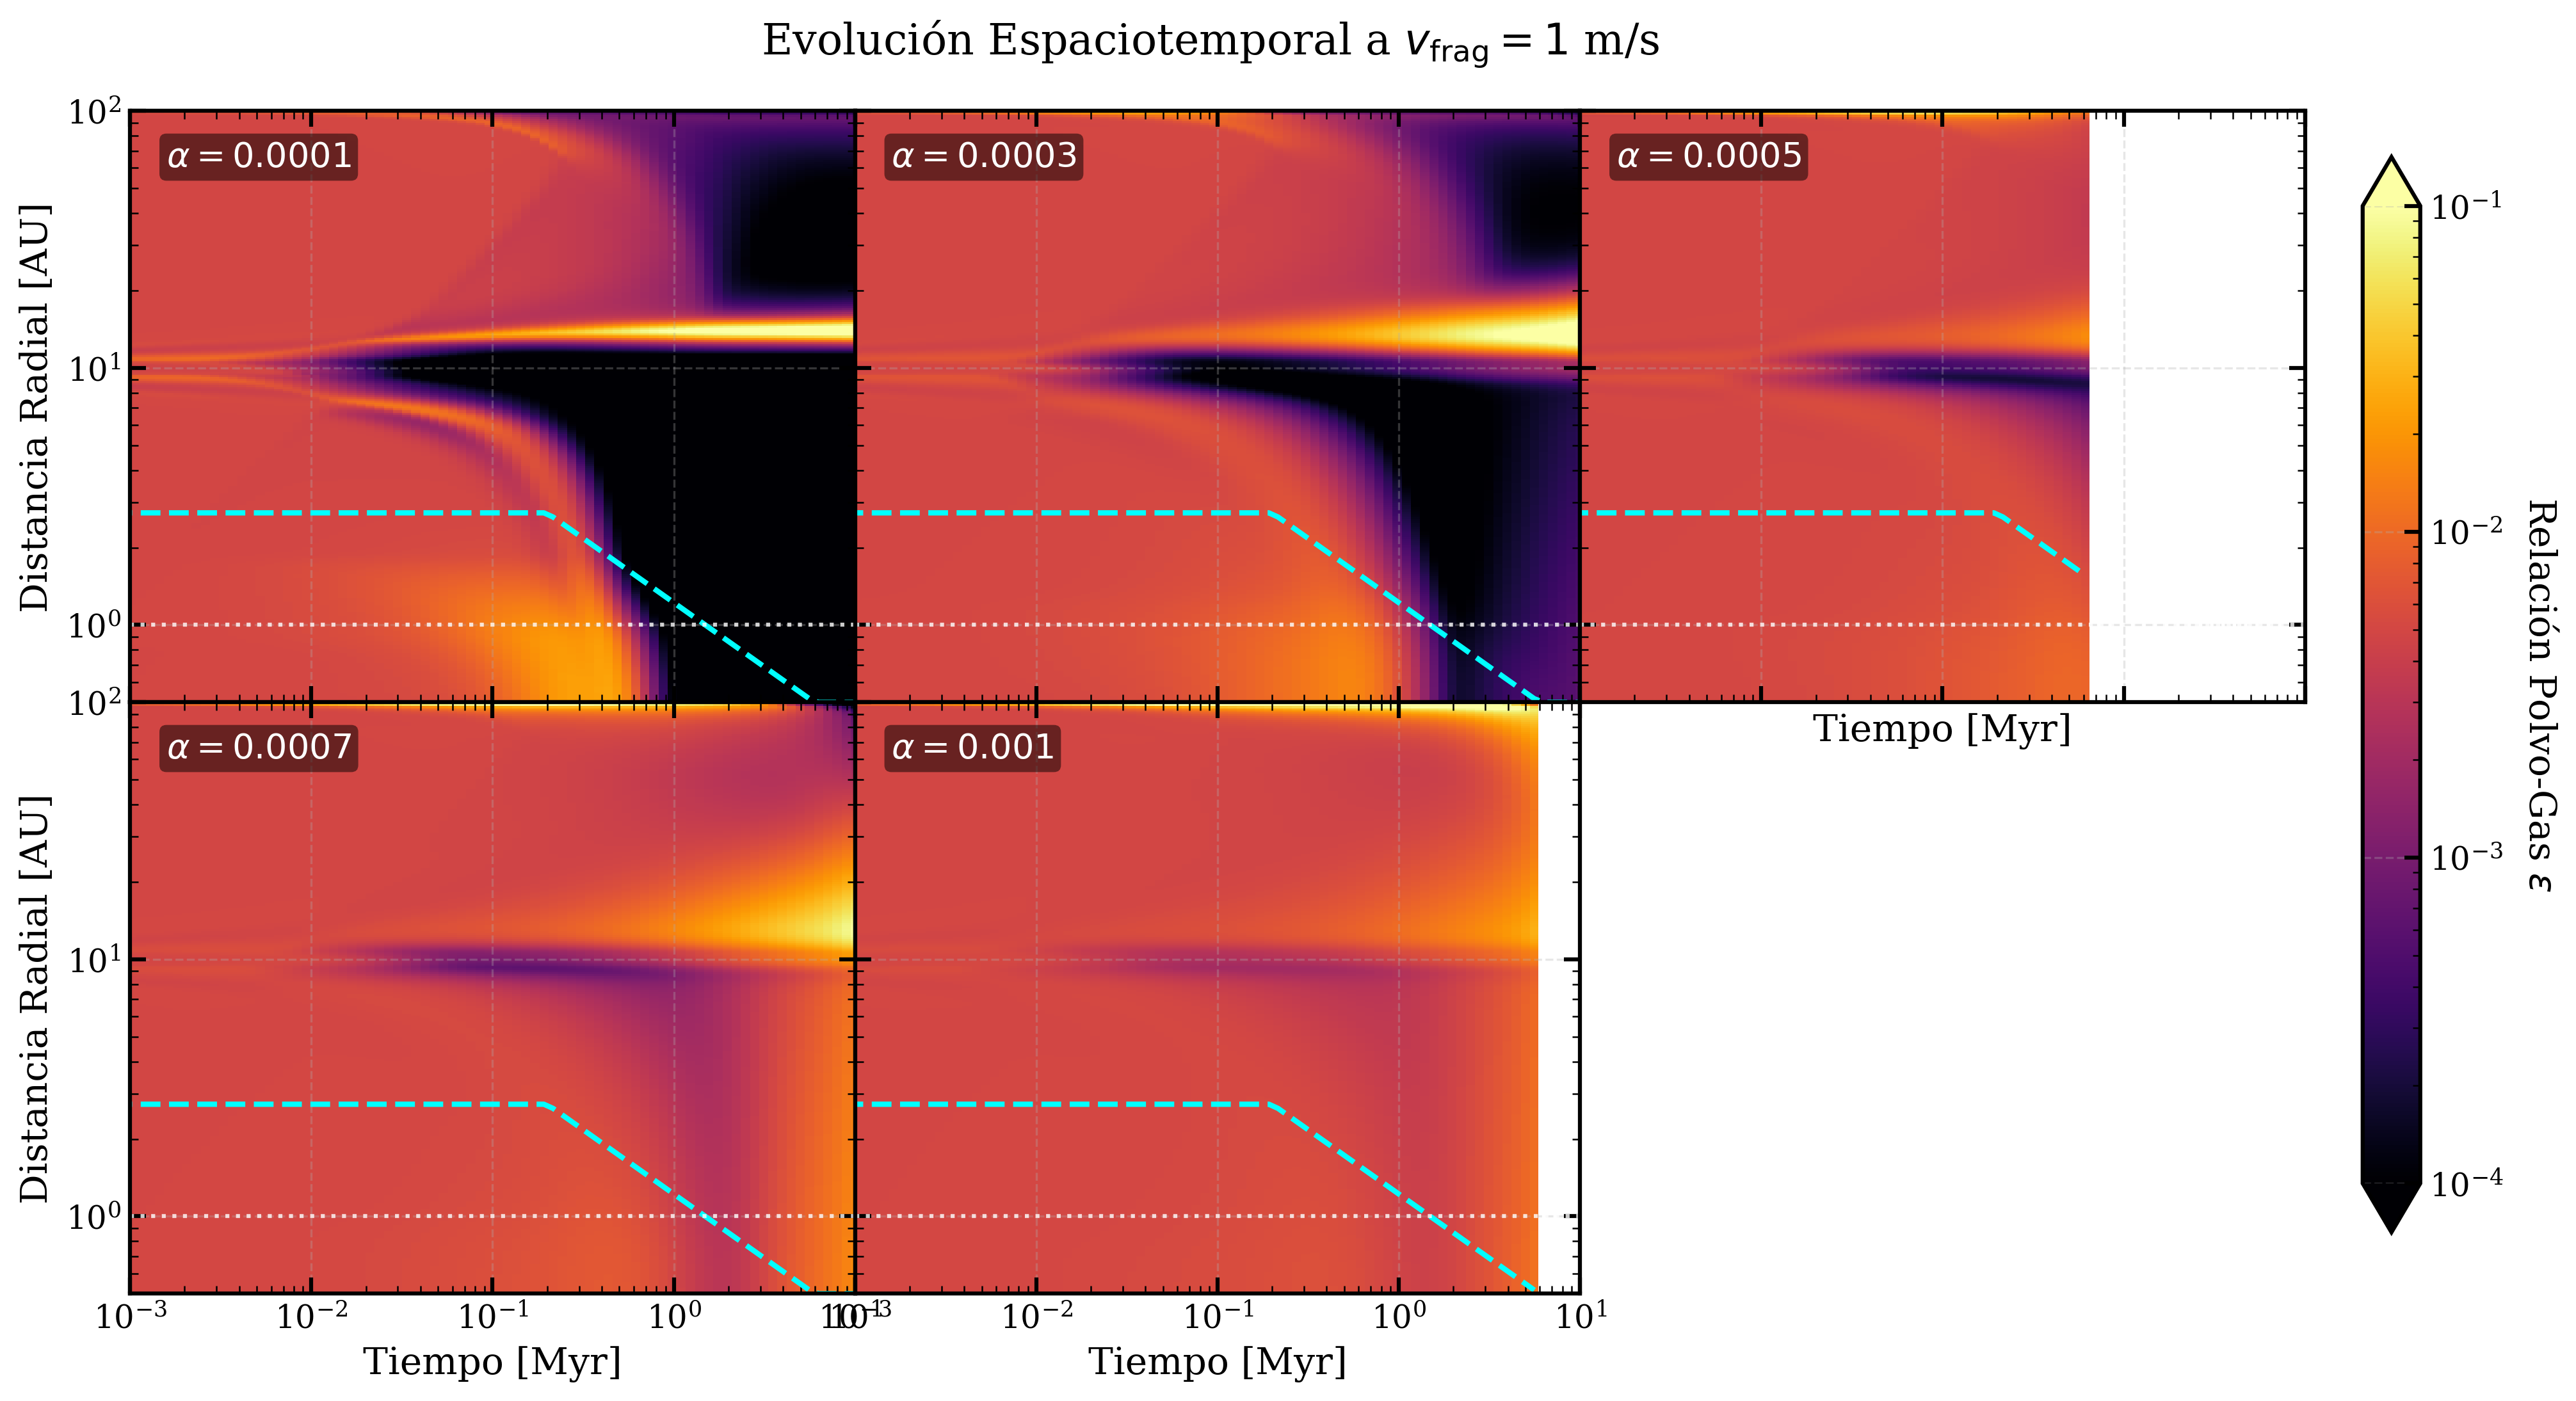
\includegraphics[width=\textwidth]{figures/apendice/hovmoller_v1.png}
    \caption{Diagrama de Hovmöller para $v_{\rm frag} = 1\text{ m/s}$ uniforme.
    La ausencia de diferencial de fragmentación elimina el evento de flushing:
    el anillo de polvo en el gap persiste estáticamente sin liberarse hacia
    el disco interior al ser cruzado por la isoterma de sublimación.}
    \label{fig:ap_hovmoller_v1}
\end{figure}

\begin{figure}[htpb]
    \centering
    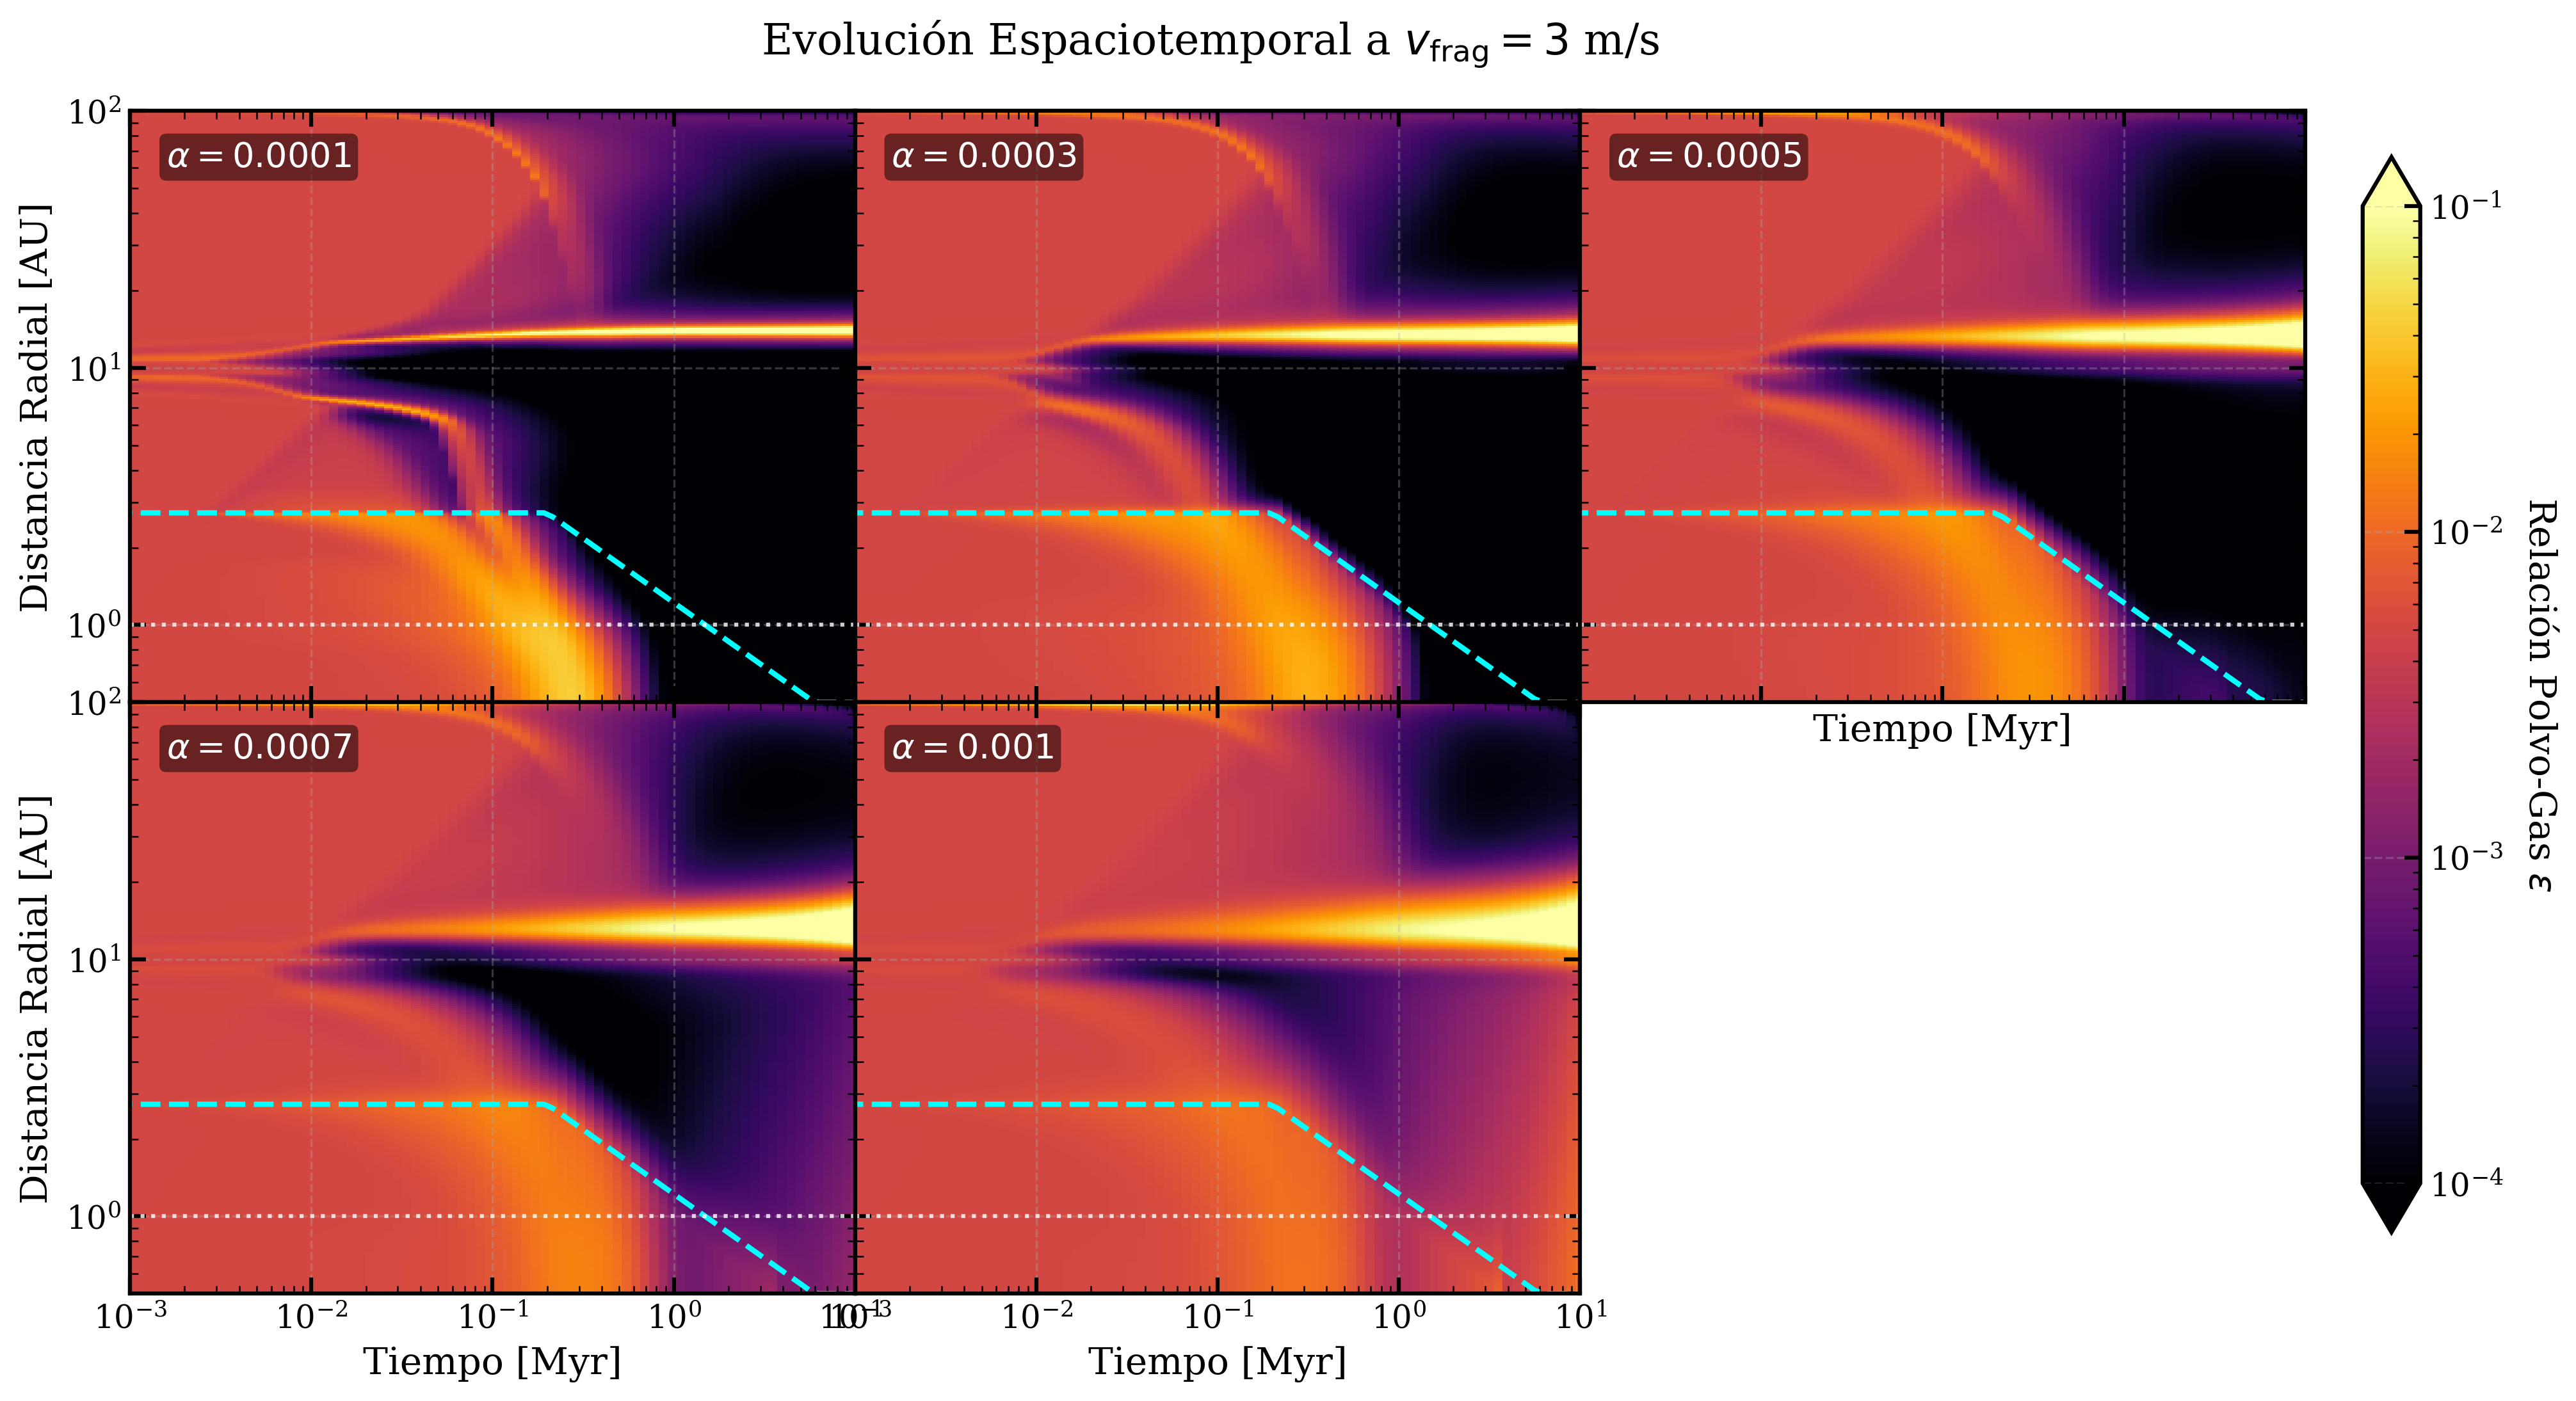
\includegraphics[width=\textwidth]{figures/apendice/hovmoller_v3.png}
    \caption{Diagrama de Hovmöller para $v_{\rm frag}^{\rm ice} = 3\text{ m/s}$.
    Se observa un flushing parcial: el diferencial reducido (factor 3 vs.\ el
    factor 10 del caso canónico) libera una fracción del material retenido al
    cruzar la snowline, produciendo un evento de acreción de menor magnitud
    que en el caso canónico.}
    \label{fig:ap_hovmoller_v3}
\end{figure}

\begin{figure}[htpb]
    \centering
    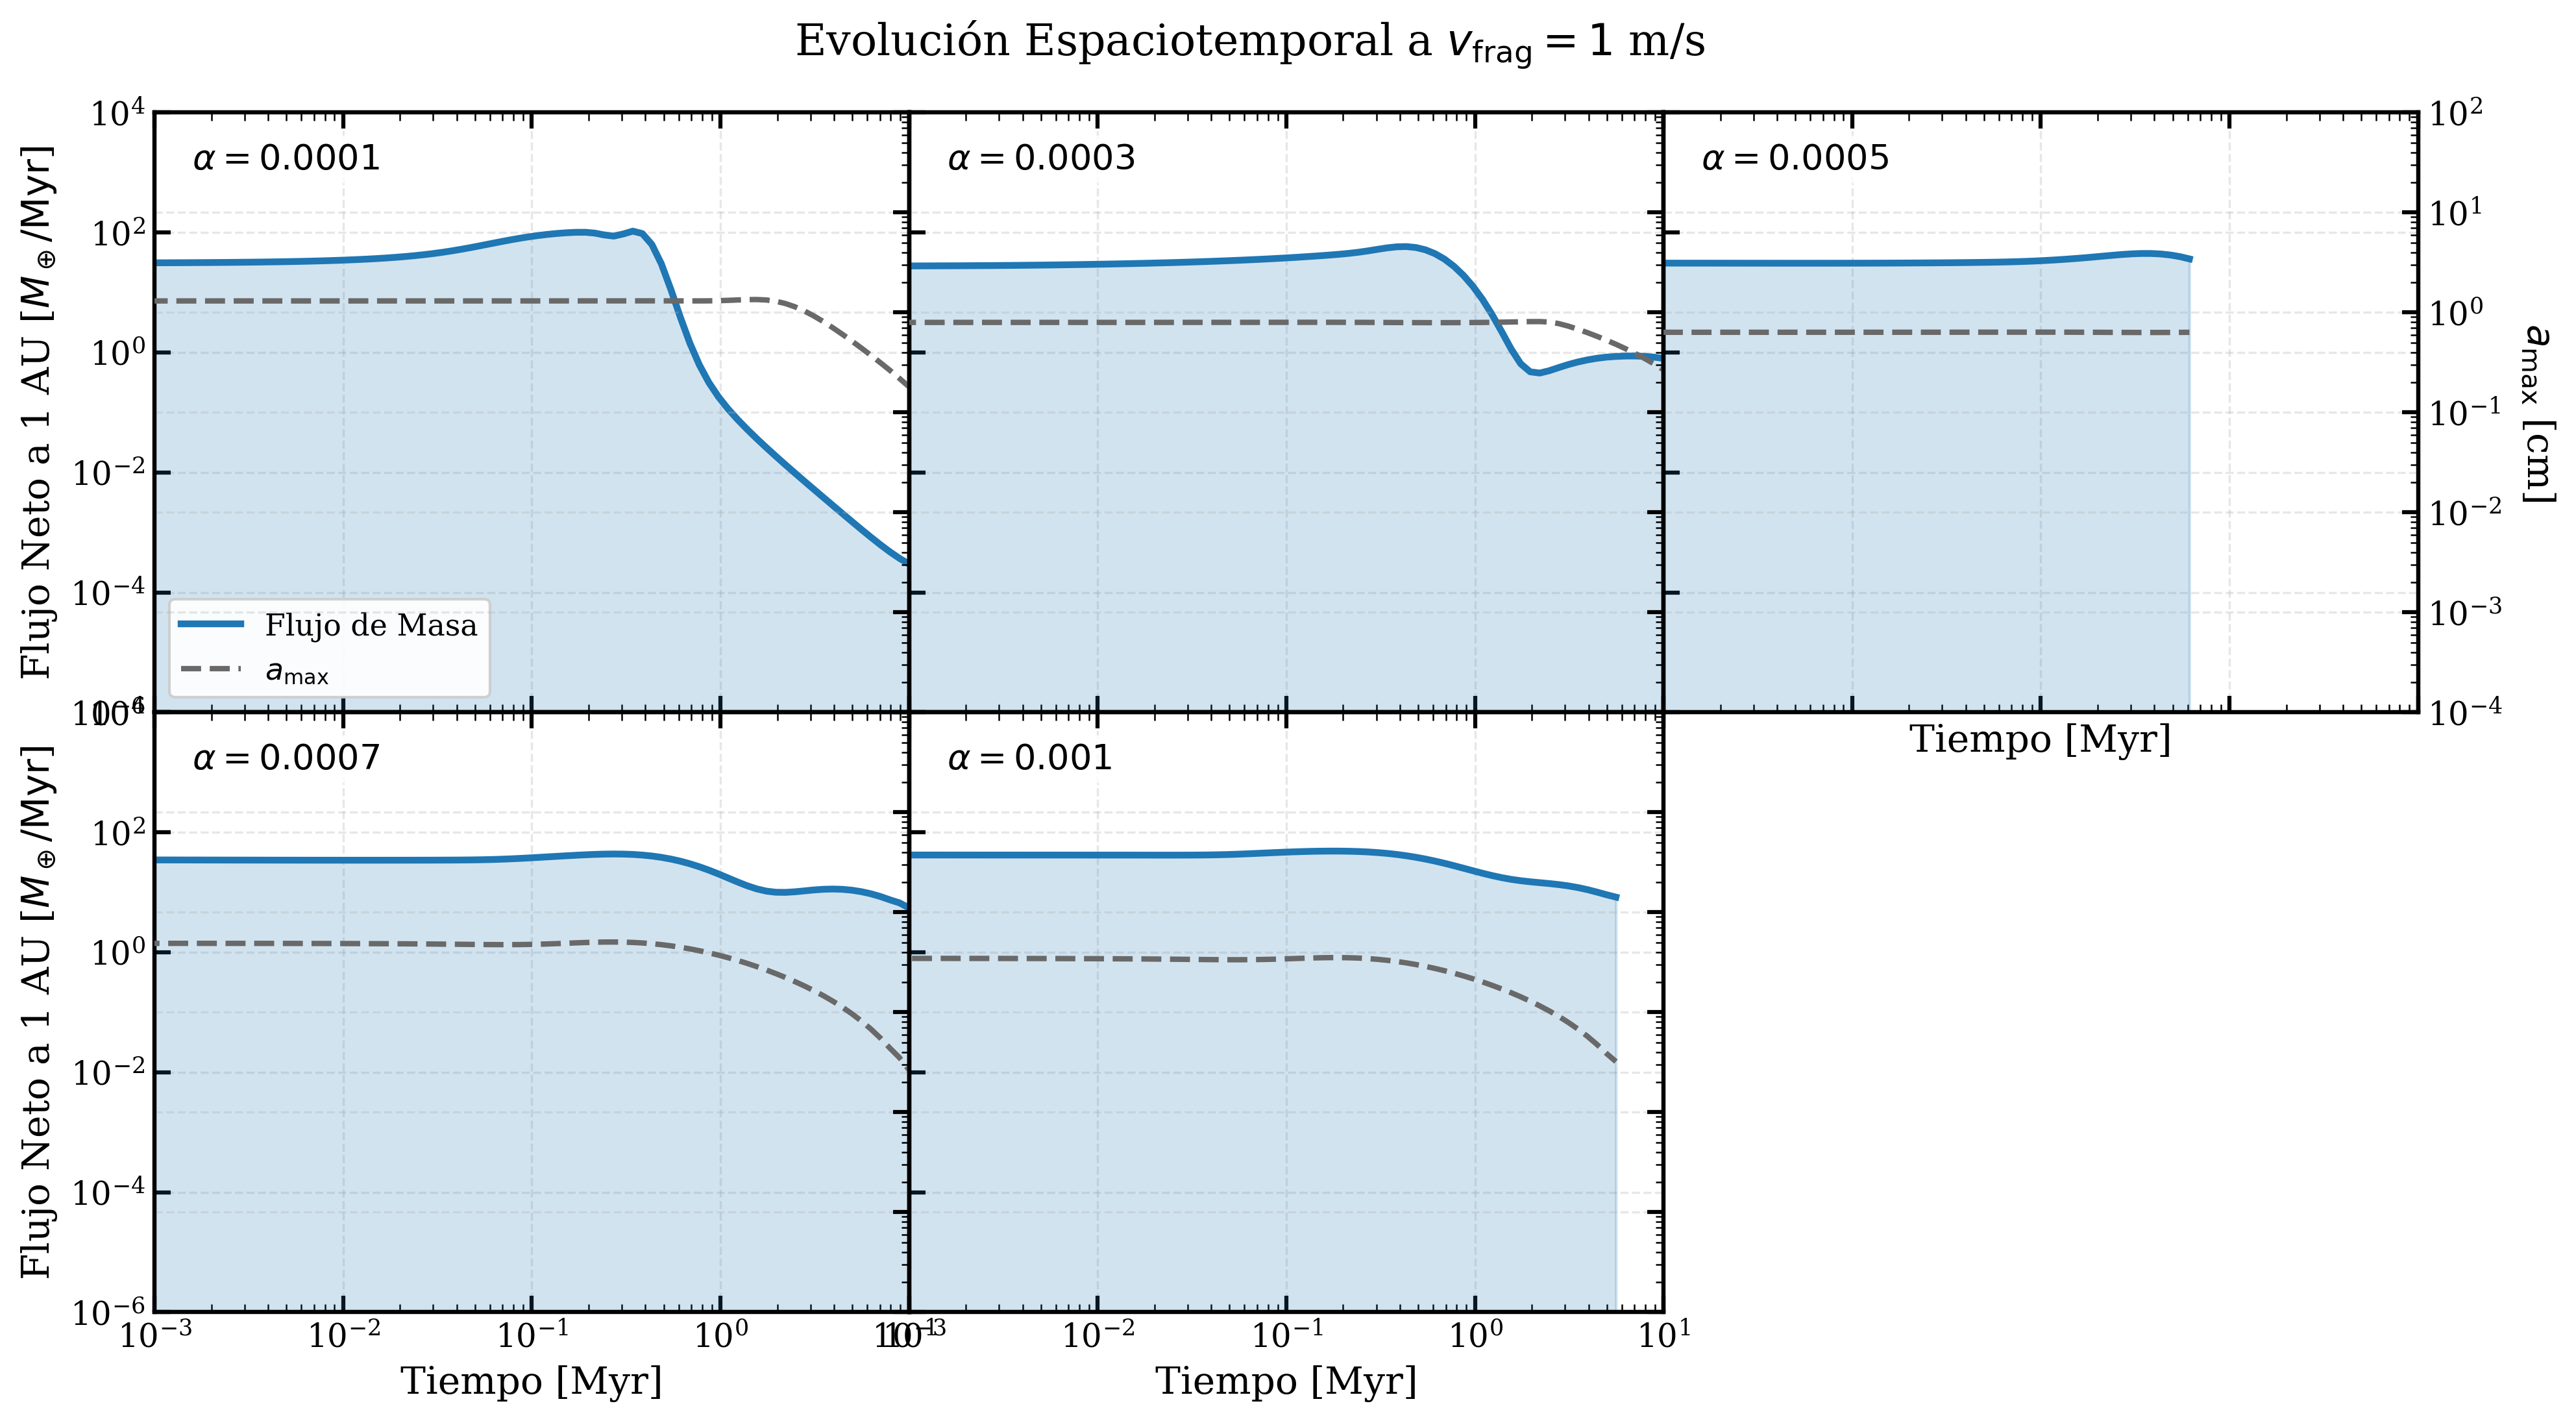
\includegraphics[width=0.49\textwidth]{figures/apendice/flux_amax_v1.png}
    \hfill
    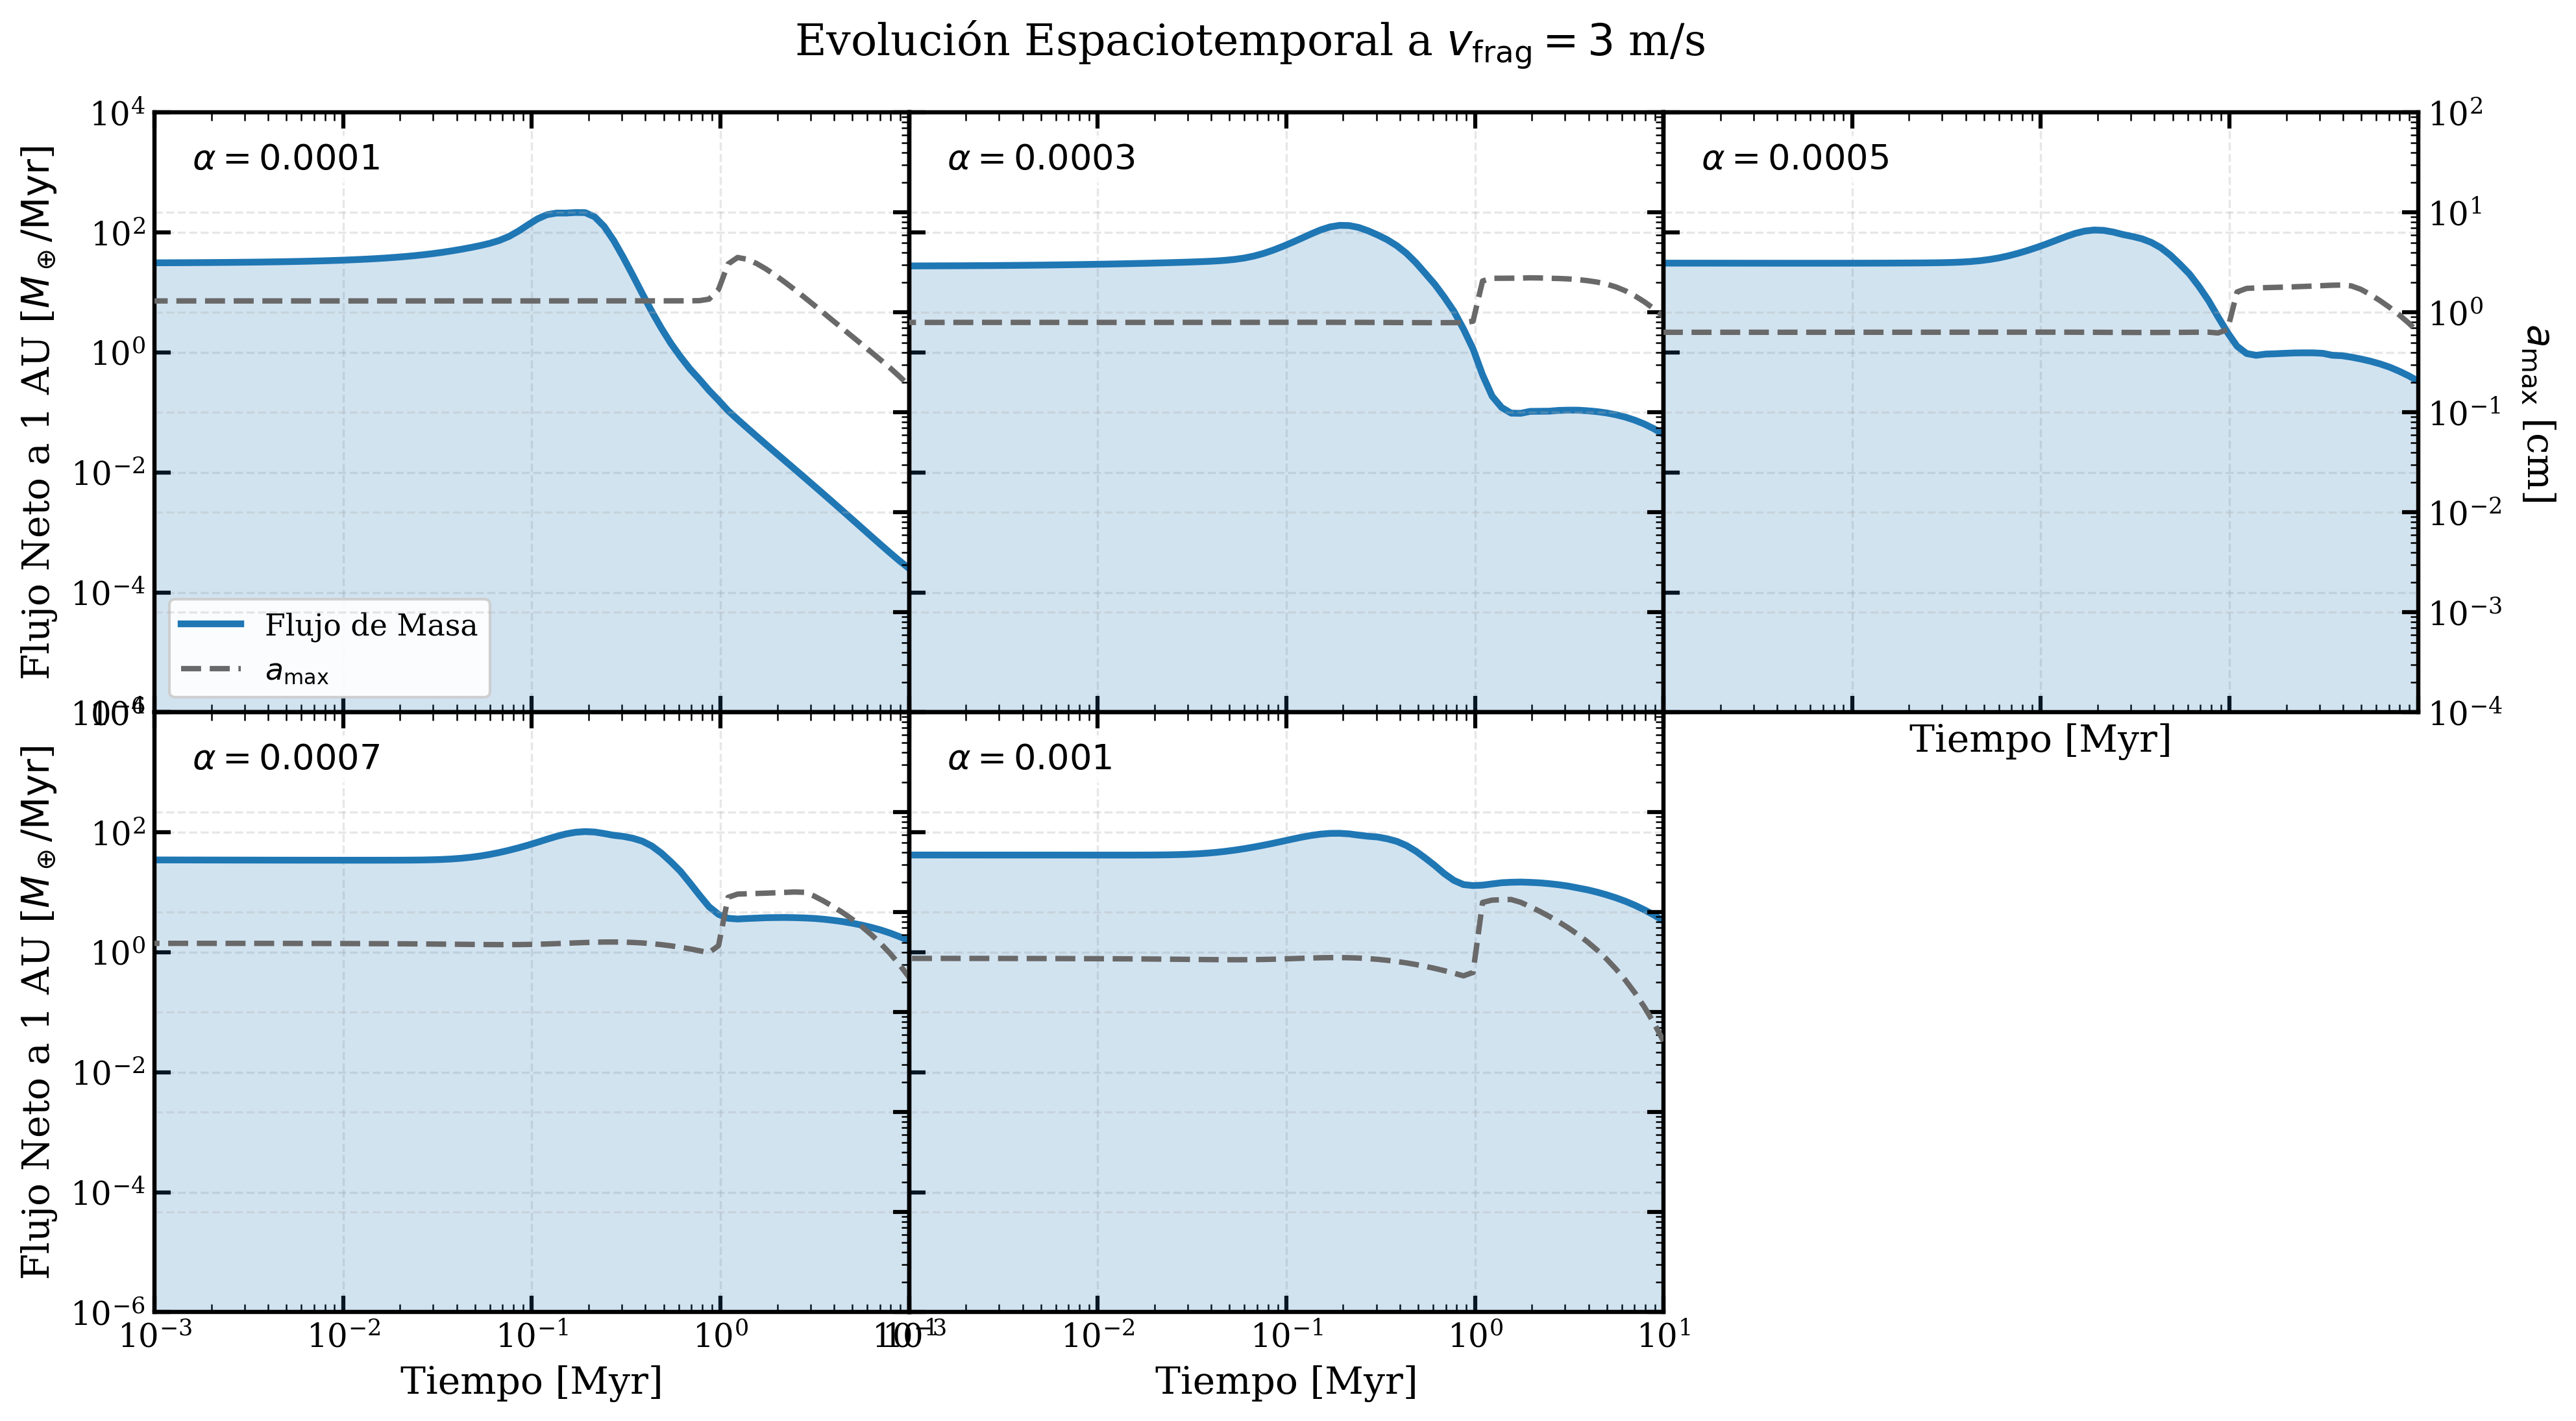
\includegraphics[width=0.49\textwidth]{figures/apendice/flux_amax_v3.png}
    \caption{Perfiles de flujo de pebbles $\dot{M}_{\rm peb}$ y tamaño máximo de
    grano $a_{\rm max}$ para $v_{\rm frag} = 1\text{ m/s}$ (izquierda) y
    $v_{\rm frag} = 3\text{ m/s}$ (derecha). En el caso de 1 m/s, el número de
    Stokes se mantiene continuo al cruzar la isoterma; en el de 3 m/s, la caída
    es moderada pero suficiente para liberar parcialmente el material del gap.}
    \label{fig:ap_flux_amax}
\end{figure}

% ---------------------------------------------------------
\section{Heatmaps del Caso Canónico ($\alpha = 0.001$)}
% ---------------------------------------------------------

Las Figuras~\ref{fig:ap_heatmap_masa} y~\ref{fig:ap_heatmap_h2o} presentan los
heatmaps de masa final y fracción de agua para el caso canónico bien definido
($\alpha = 0.001$, $v_{\rm frag} = 10\text{ m/s}$, $M_0 = 10^{-4}\,M_\oplus$),
mostrando la "Isla de Crecimiento" con mayor resolución que el diagrama de burbujas
de la Figura~\ref{fig:bubble_v10}.

\begin{figure}[htpb]
    \centering
    
\includegraphics[width=0.49\textwidth]{figures/apendice/heatmap_masa.png}
    \hfill
    
\includegraphics[width=0.49\textwidth]{figures/apendice/heatmap_h2o.png}
    \caption{\textit{Izquierda:} Heatmap de masa final $\log(M_c/M_\oplus)$ en
    función de la posición $r_{\rm gap}$ (eje X) y la masa $M_{\rm gap}$ (eje Y)
    del gap planetario.
    \textit{Derecha:} Heatmap de la fracción de agua $f_{\rm H_2O}$ para los
    mismos parámetros.
    La banda de crecimiento exitoso ($M_{\rm gap} \sim 0.1\,M_{\rm Jup}$) es
    claramente visible, así como la correlación entre alta masa final y baja
    fracción de agua en el régimen de filtrado óptimo.}
    \label{fig:ap_heatmap_masa}
    \label{fig:ap_heatmap_h2o}
\end{figure}

% ---------------------------------------------------------
\section{Cronología del Gap: Gaps Retrasados}
% ---------------------------------------------------------

\begin{figure}[htpb]
    \centering
    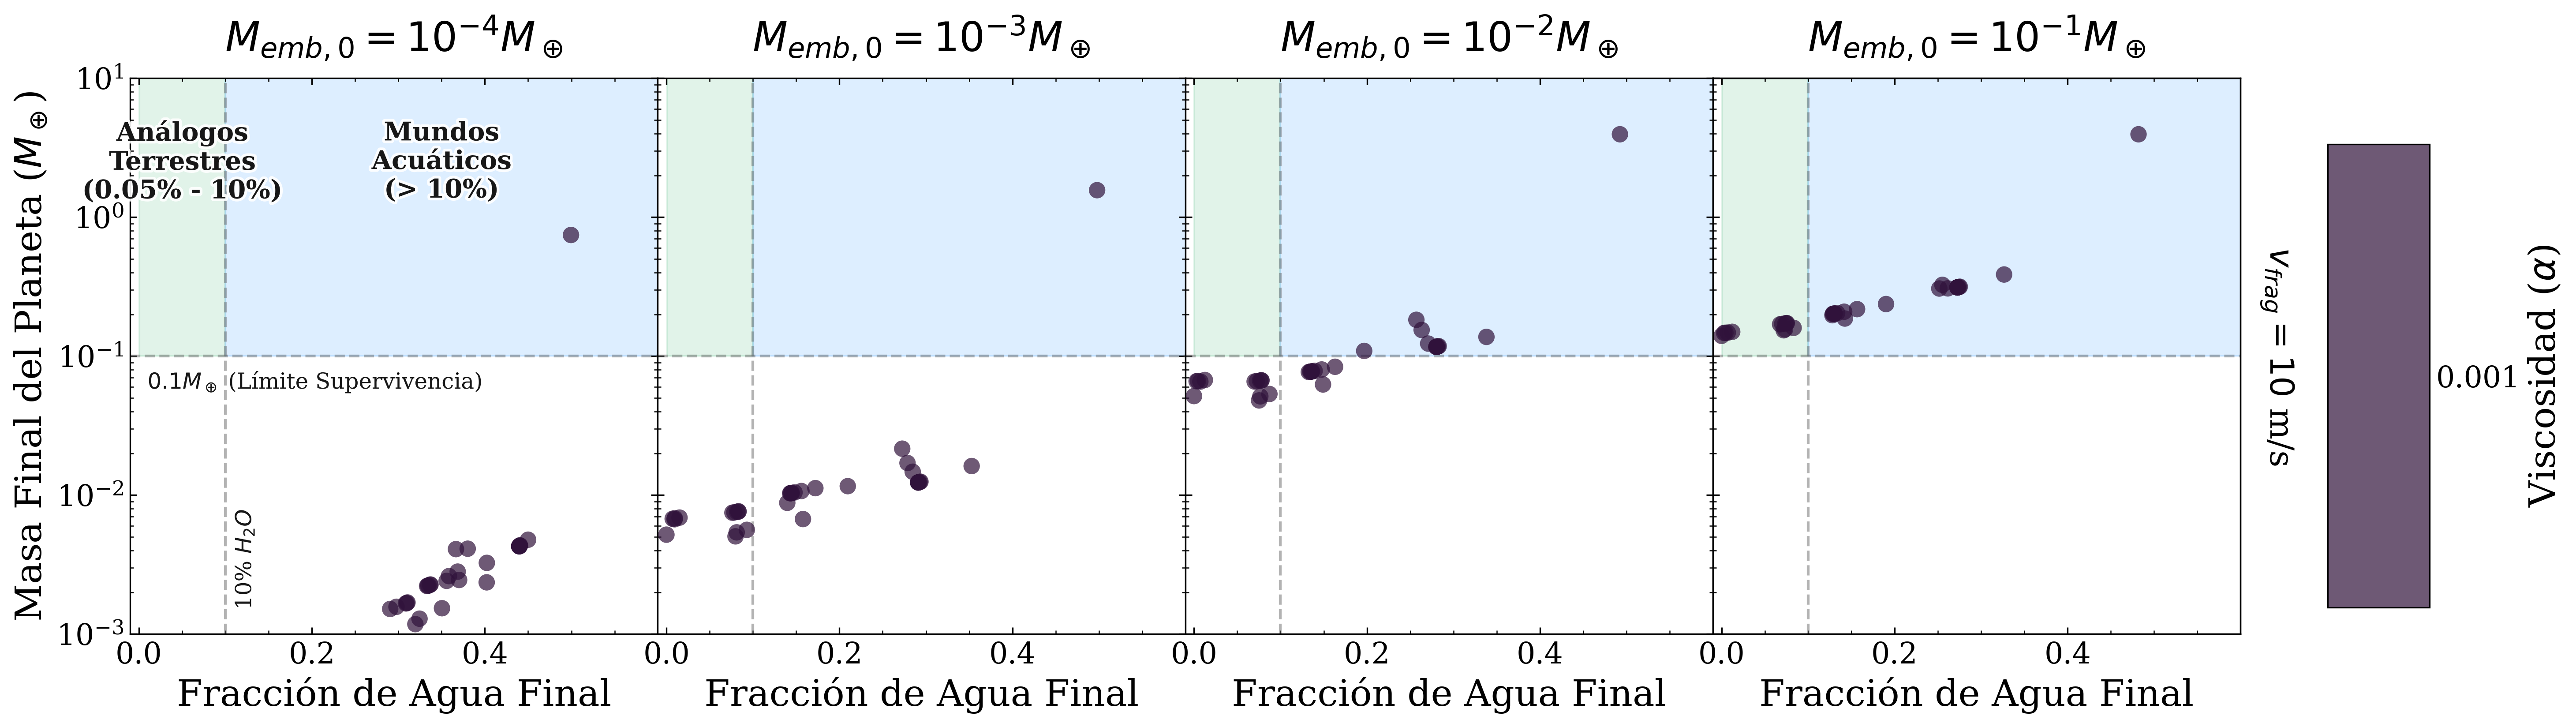
\includegraphics[width=\textwidth]{figures/apendice/population_delayed.png}
    \caption{Curvas de crecimiento del embrión para distintos tiempos de inserción
    del gap $t_{\rm gap}$ (colores). El gap se ubica a 10 AU con
    $M_{\rm gap} = 0.1\,M_{\rm Jup}$ y $\alpha = 0.001$.
    Para $t_{\rm gap} \ge 2\text{ Myr}$, la mayor parte del inventario sólido
    primordial ya ha derivado hacia la estrella antes de que el gap se forme,
    eliminando el reservorio de material disponible para el evento de flushing.}
    \label{fig:ap_delayed}
\end{figure}

% ---------------------------------------------------------
\section{Distribución Volumétrica en Discos Sinusoidales}
% ---------------------------------------------------------

\begin{figure}[htpb]
    \centering
    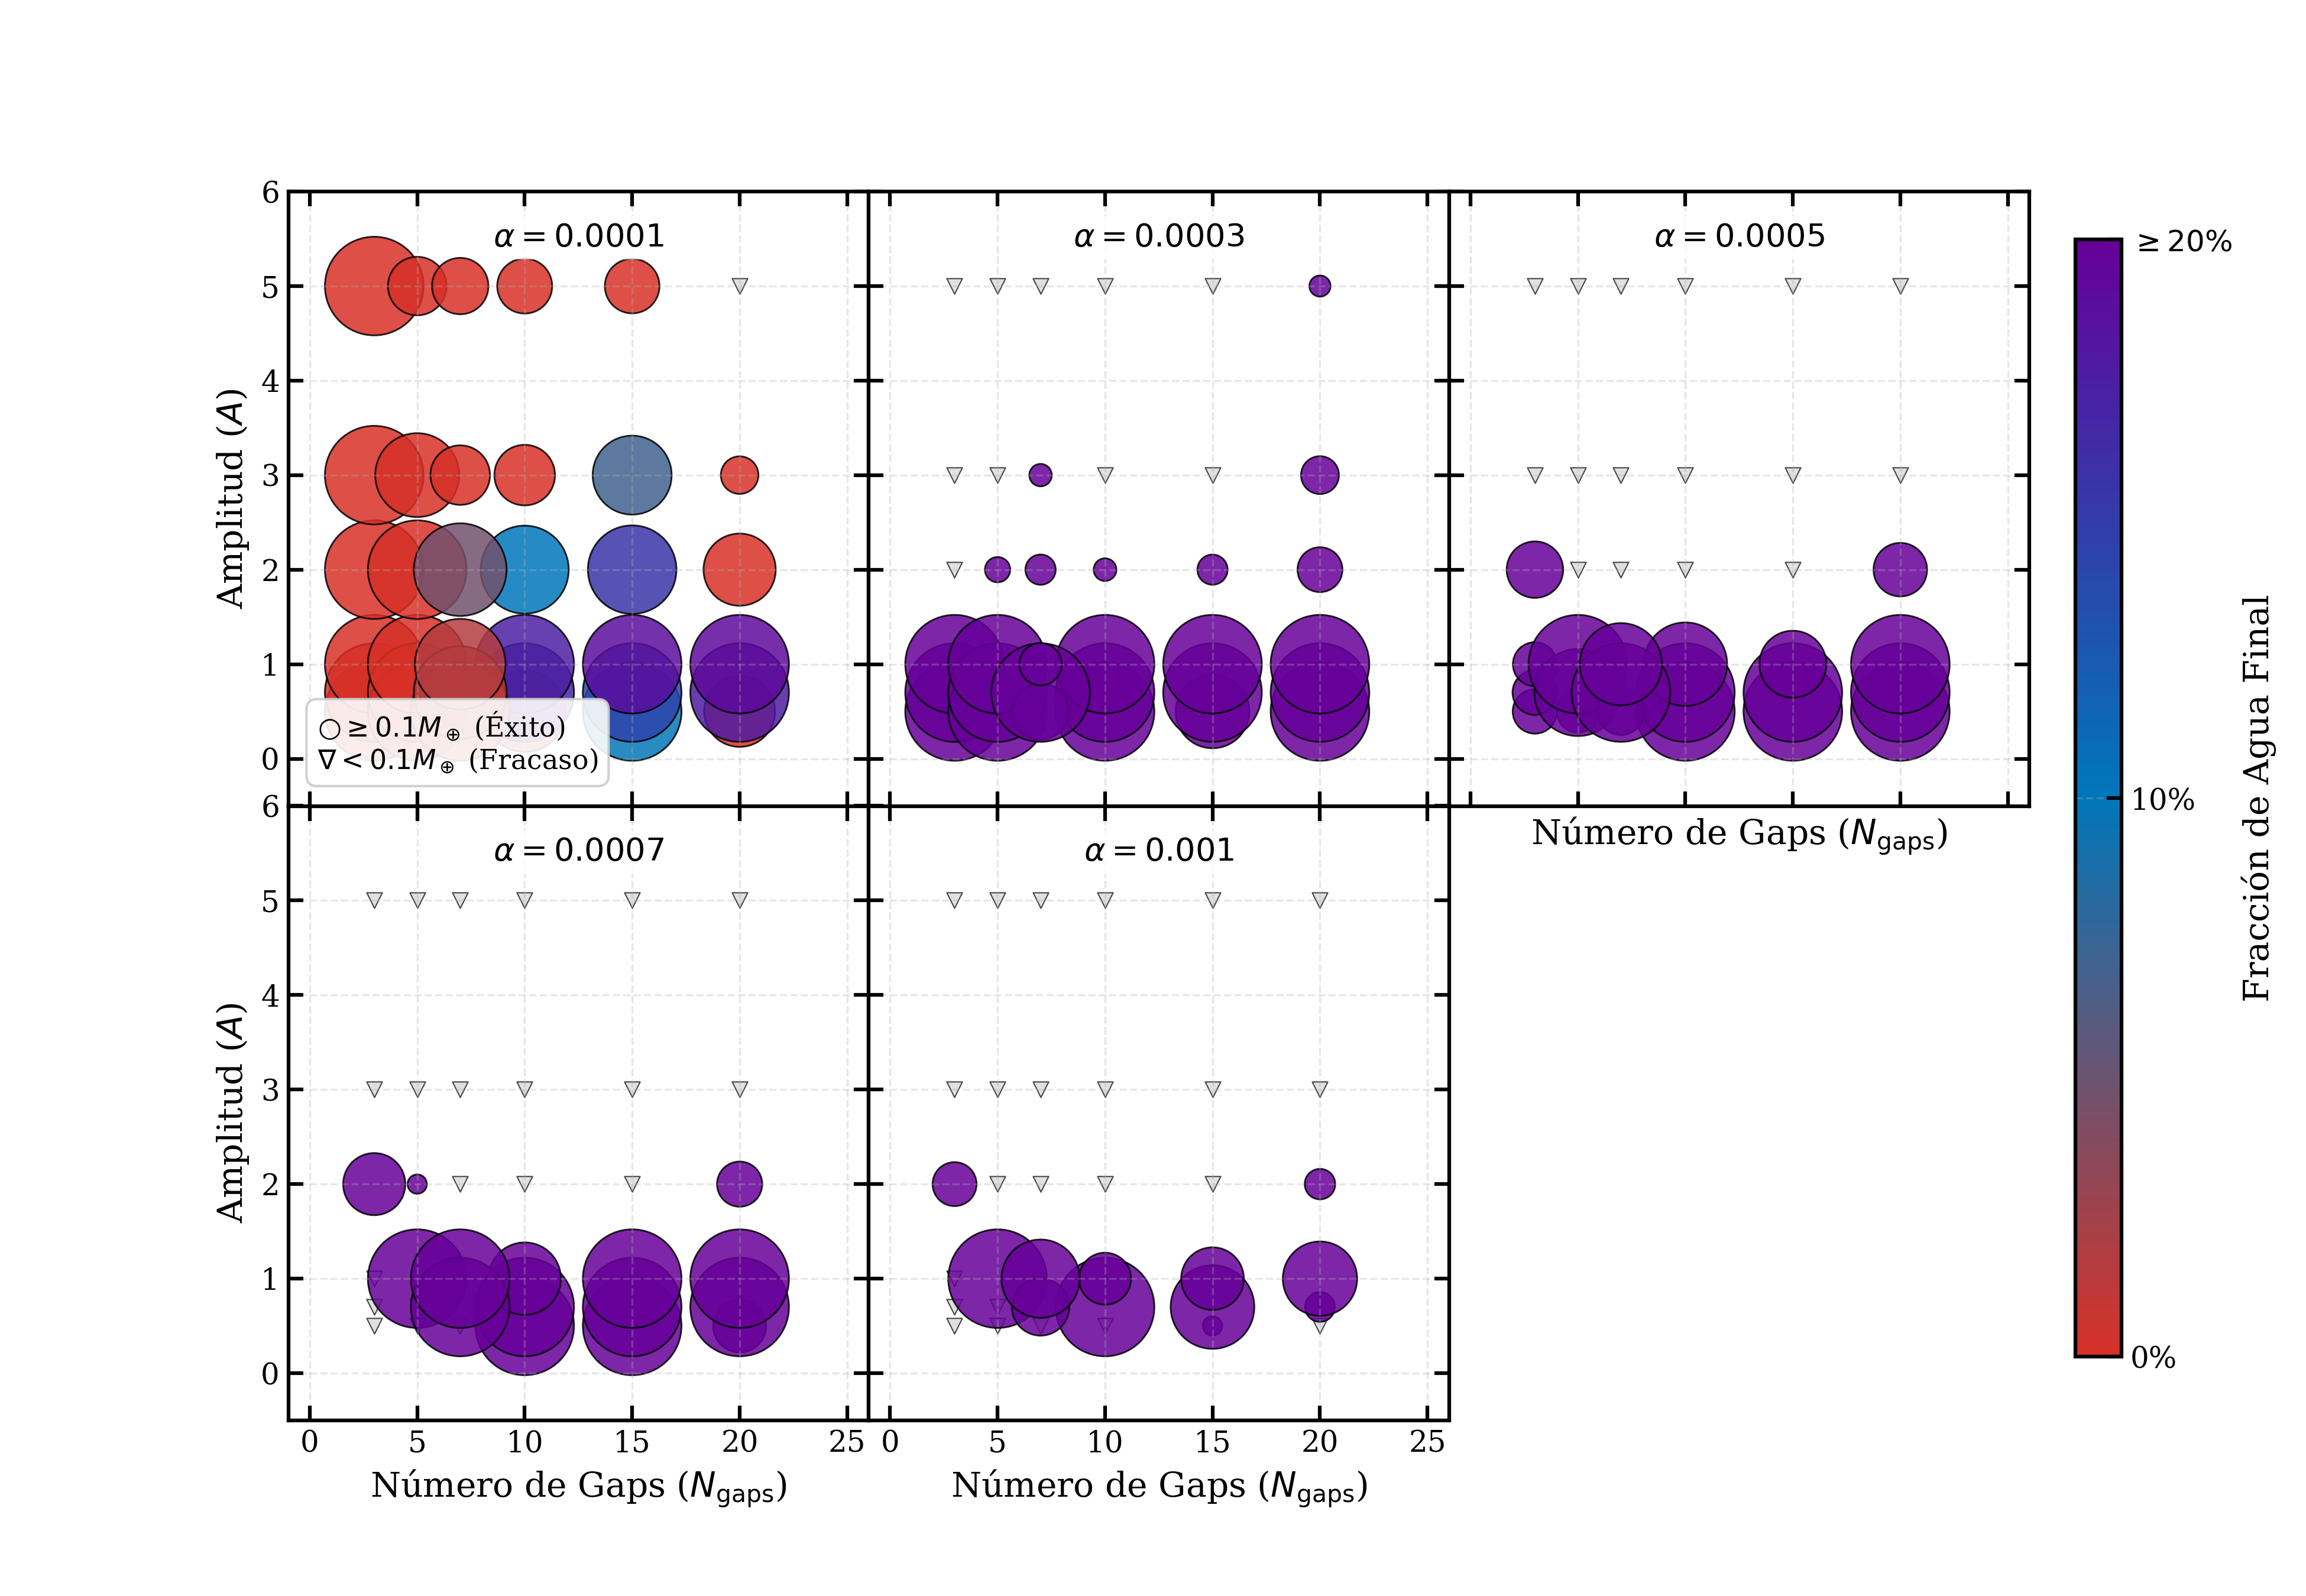
\includegraphics[width=\textwidth]{figures/apendice/bubble_sinusoidal_v10.png}
    \caption{Diagrama de burbujas para configuraciones sinusoidales con
    $v_{\rm frag} = 10\text{ m/s}$. El diámetro de cada punto es proporcional
    a $M_c$; el color indica $f_{\rm H_2O}$. La ausencia de burbujas grandes
    en el régimen de alta amplitud ($A \ge 3.0$) confirma que las subestructuras
    periódicas profundas suprimen la formación de embriones masivos en las
    regiones interiores del disco.}
    \label{fig:ap_bubble_sin}
\end{figure}

% ---------------------------------------------------------
\section{Validación Numérica: Sensibilidad a $M_{\rm cross}$}
% ---------------------------------------------------------

Para verificar que los resultados no son artefactos de la parametrización específica
de la migración de la isoterma, se repitieron simulaciones variando el parámetro
$M_{\rm cross}$, que controla el tiempo de cruce de la snowline en el modelo de
Oka \& Hartmann. Las Figuras~\ref{fig:ap_mcross_masa} y~\ref{fig:ap_mcross_h2o}
muestran que la masa final y la fracción de agua son insensibles a variaciones de
$M_{\rm cross}$ dentro de rangos físicamente plausibles, confirmando la universalidad
del mecanismo.

\begin{figure}[htpb]
    \centering
    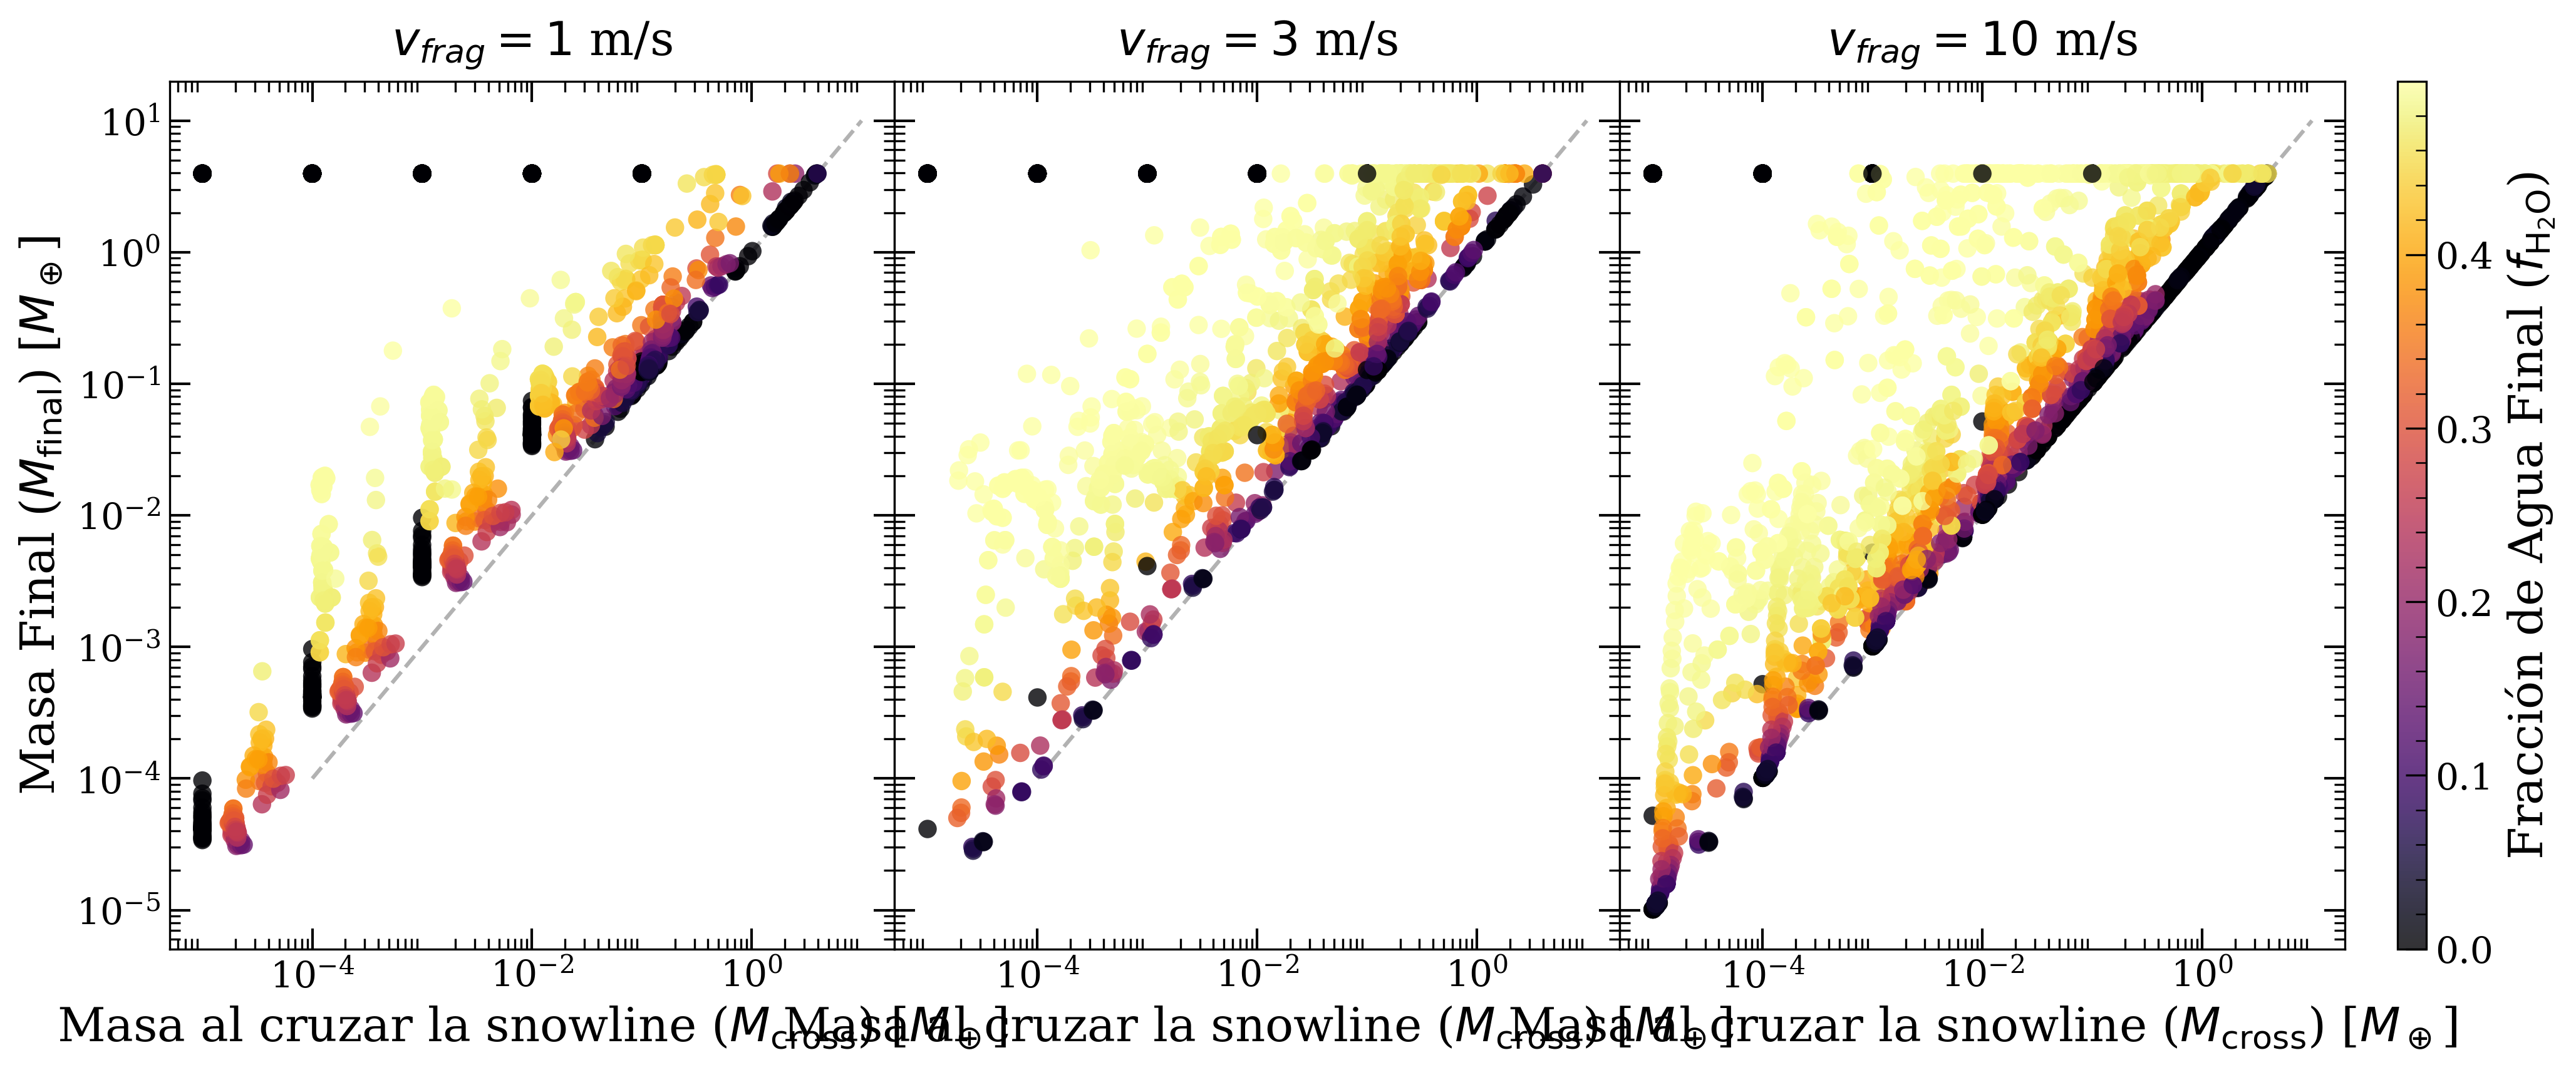
\includegraphics[width=0.49\textwidth]{figures/apendice/FigC_Mcross.png}
    \hfill
    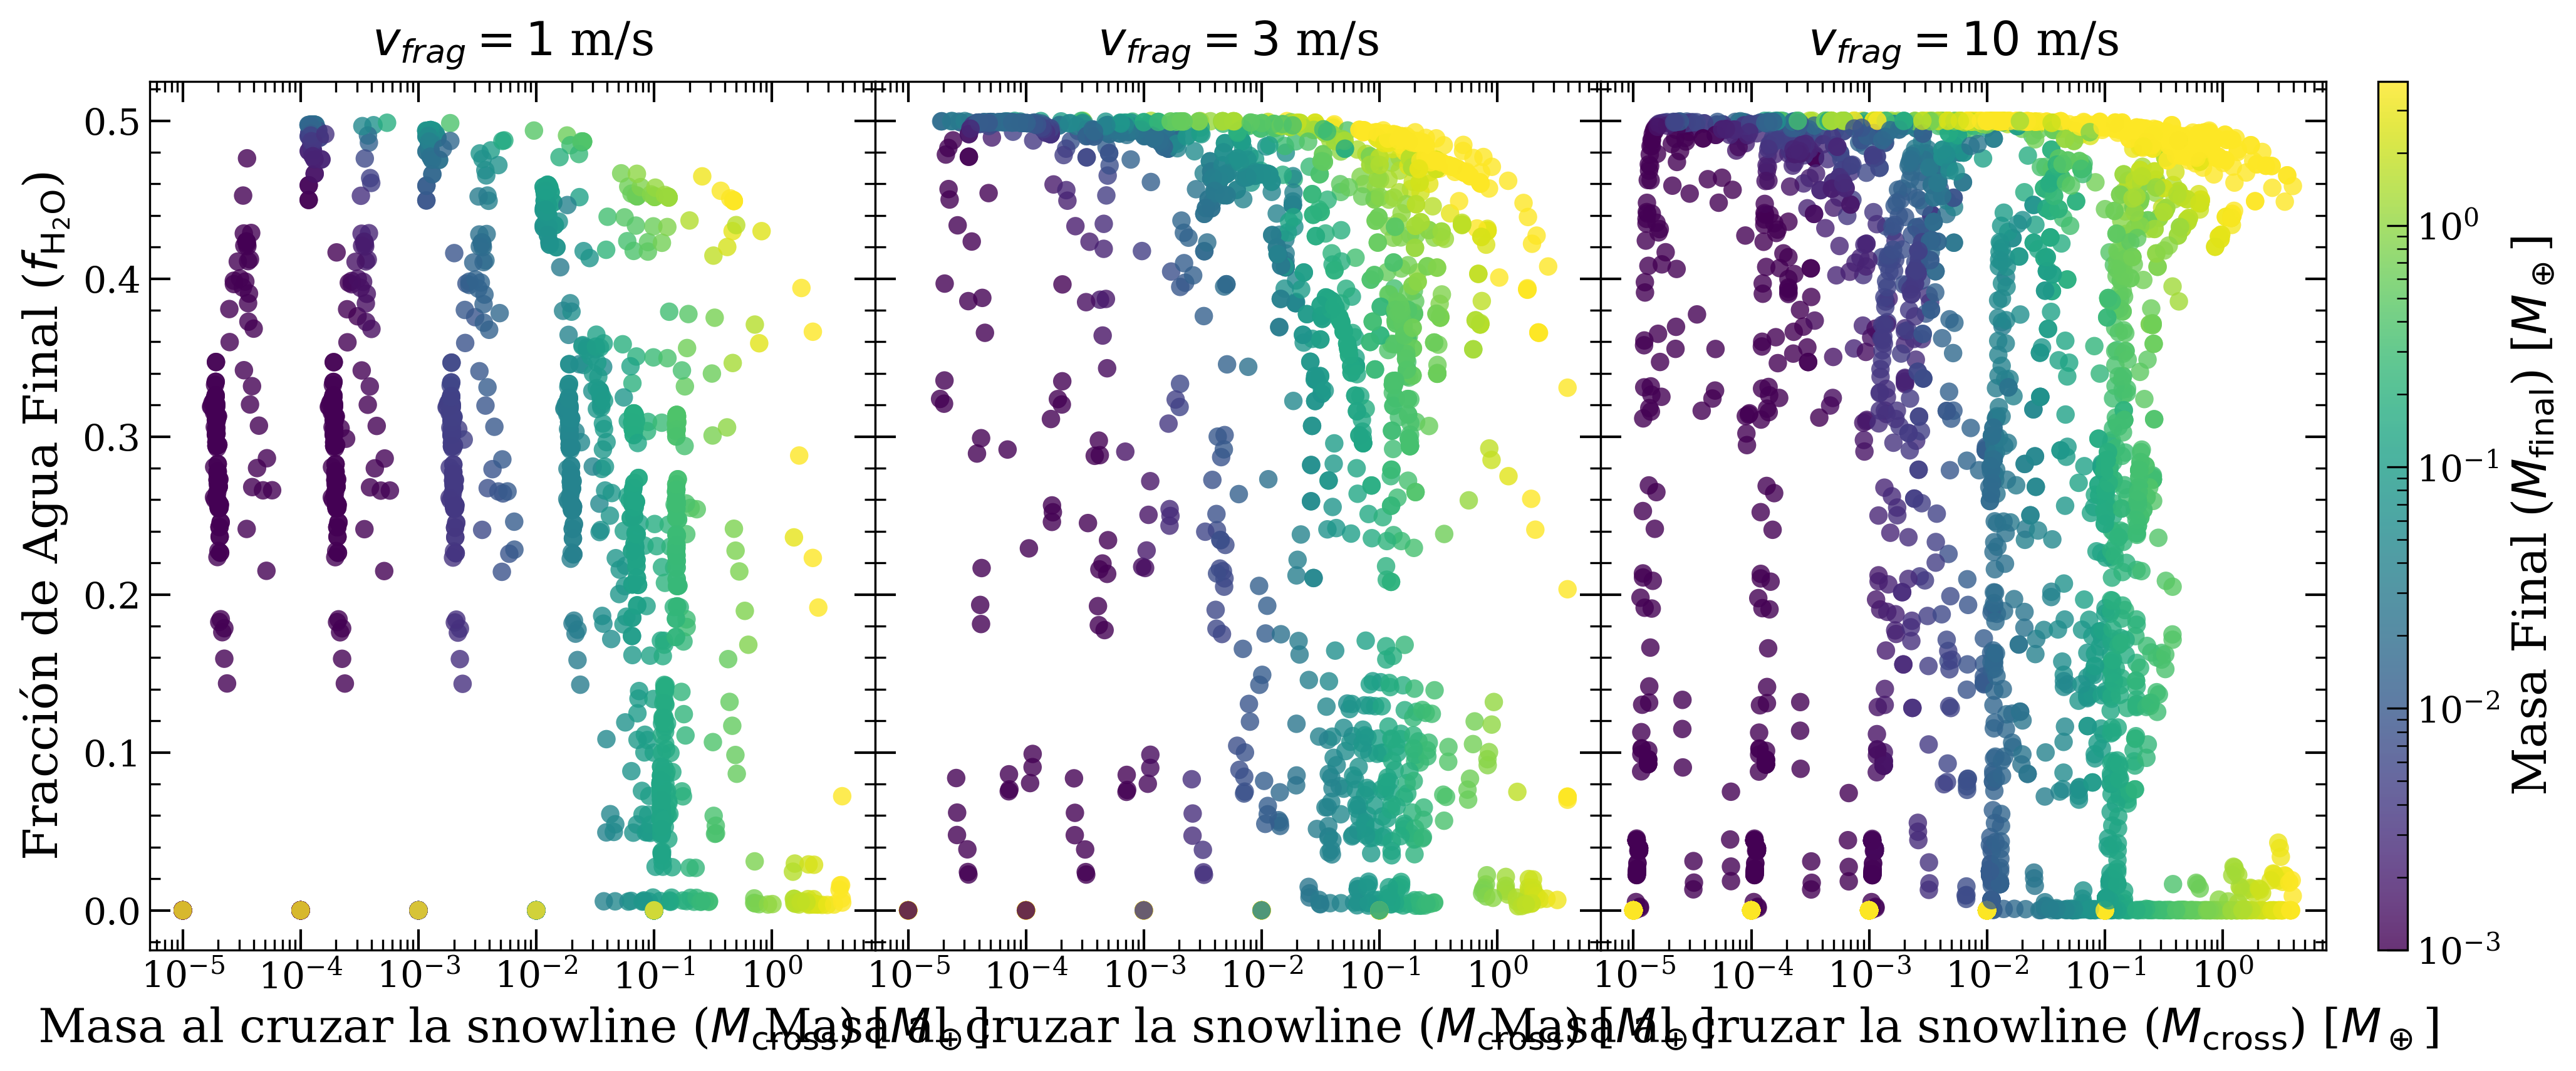
\includegraphics[width=0.49\textwidth]{figures/apendice/FigD_Mcross.png}
    \caption{\textit{Izquierda:} Masa final $M_c$ en función de $M_{\rm cross}$
    para distintas configuraciones de gap.
    \textit{Derecha:} Fracción de agua $f_{\rm H_2O}$ en función de $M_{\rm cross}$.
    La dispersión en ambas variables es menor al 5\% para el rango de
    $M_{\rm cross}$ explorado, validando la robustez numérica de los resultados.}
    \label{fig:ap_mcross_masa}
    \label{fig:ap_mcross_h2o}
\end{figure}

% % Apéndice B

\chapter{Derivaciones Adicionales}

Segundo apéndice de ejemplo.


% --- REFERENCIAS BIBLIOGRÁFICAS ---
\cleardoublepage
\addcontentsline{toc}{chapter}{Bibliografía}
\cleardoublepage
\footnotesize
\setlength{\bibsep}{0pt}

% Reemplaza plainnat por el estilo de astronomía
\bibliographystyle{AASjournal}% También puedes probar con {aasjournal} o {apalike}

\bibliography{biblio}

\end{document}